\documentclass[review,3p]{elsarticle}
%\documentclass[preprint,3p]{elsarticle}

\usepackage{lineno,hyperref}
\modulolinenumbers[5]

\journal{Information Science}

%%%%%%%%%%%%%%%%%%%%%%%
%% Elsevier bibliography styles
%%%%%%%%%%%%%%%%%%%%%%%
%% To change the style, put a % in front of the second line of the current style and
%% remove the % from the second line of the style you would like to use.
%%%%%%%%%%%%%%%%%%%%%%%

%% Numbered
%\bibliographystyle{model1-num-names}

%% Numbered without titles
%\bibliographystyle{model1a-num-names}

%% Harvard
%\bibliographystyle{model2-names.bst}\biboptions{authoryear}

%% Vancouver numbered
%\usepackage{numcompress}\bibliographystyle{model3-num-names}

%% Vancouver name/year
%\usepackage{numcompress}\bibliographystyle{model4-names}\biboptions{authoryear}

%% APA style
%\bibliographystyle{model5-names}\biboptions{authoryear}

%% AMA style
%\usepackage{numcompress}\bibliographystyle{model6-num-names}
\usepackage{xcolor}
%% `Elsevier LaTeX' style
\bibliographystyle{elsart-num-sort}
%%%%%%%%%%%%%%%%%%%%%%%

\newcommand{\EAS}{{\sc ea}s}
\newcommand{\CDE}{c{\sc de}}
\newcommand{\DE}{{\sc de}}
\newcommand{\HMR}{{\sc hmr}}
\newcommand{\METCO}{\mbox{\sc{metco}}{}}
\newcommand{\NP}{{\sc np}}

\begin{document}

\begin{frontmatter}

\title{Improving the Vector Generation Strategy of Differential \\ Evolution for Large-Scale Optimization}
%\tnotetext[mytitlenote]{Fully documented templates are available in the elsarticle package on \href{http://www.ctan.org/tex-archive/macros/latex/contrib/elsarticle}{CTAN}.}

%% or include affiliations in footnotes:
\author[label1]{Carlos Segura\corref{cor1}}
\ead{carlos.segura@cimat.mx}

\author[label2]{Carlos A. Coello Coello}
\ead{ccoello@cs.cinvestav.mx}

\author[label3]{Alfredo G. Hern\'andez-D\'iaz}
\ead{agarher@upo.es}

\cortext[cor1]{Corresponding author. Tel.: + 52 473 732 7155}
\address[label1]{Area of Computer Science, Centre for Research in Mathematics (CIMAT), Callej\'on Jalisco s/n, Mineral de Valenciana, Guanajuato, Guanajuato 36240, Mexico}
\address[label2]{Evolutionary Computation Group, Department of Computer Science, Center of Research and Advanced Studies, National Polytechnic Institute, Mexico City 07300, Mexico}
\address[label3]{Department of Economics, Quantitative Methods and Economic History, Pablo de Olavide University, Seville, Spain}

\begin{abstract}
Differential Evolution is an efficient metaheuristic for continuous optimization that suffers from the curse of dimensionality.
A large amount of experimentation has allowed researchers to find
several potential weaknesses in Differential Evolution.
Some of these weaknesses do not significantly affect its performance when dealing with low-dimensional problems,
so the research community has not paid much attention to them.
The aim of this paper is to provide a better insight into the reasons of the curse of dimensionality
and to propose techniques to alleviate this problem.
Two different weaknesses are revisited and schemes for dealing with them are devised.
The schemes increase the diversity of trial vectors and improve on the exploration capabilities of Differential Evolution.
\textcolor{red}{
Some important mathematical properties induced by our proposals are studied and compared against the ones of related schemes.
Experimentation with a set of problems with up to 1000 dimensions and with several variants of Differential Evolution
shows that the analyzed weaknesses
significantly affect the performance of Differential Evolution when used on high-dimensional optimization problems.
The gains of the proposals appear when too exploitative schemes are used.
Our proposals enable the achievement of high-quality solution with small populations,
meaning that the most significant advantages emerge when dealing with large-scale optimization problems,
where the benefits of using small populations have been previously shown.
}
\end{abstract}

\begin{keyword}
Differential evolution \sep diversity preservation \sep global numerical optimization \sep large-scale optimization \sep vector generation strategy
\end{keyword}

\end{frontmatter}

\linenumbers

\section{Introduction}
% The very first letter is a 2 line initial drop letter followed
% by the rest of the first word in caps.
%
% fOrm to use if the first word consists of a single letter:
% \IEEEPARstart{A}{demo} file is ....
%
% form to use if you need the single drop letter followed by
% normal text (unknown if ever used by IEEE):
% \IEEEPARstart{A}{}demo file is ....
%
% Some journals put the first two words in caps:
% \IEEEPARstart{T}{his demo} file is ....
%
% Here we have the typical use of a "T" for an initial drop letter
% and "HIS" in caps to complete the first word.
Differential Evolution (\DE{})~\cite{Storn:95} is an efficient population-based metaheuristic initially designed
for continuous optimization.
%
From its inception, it has yielded remarkable results in several optimization competitions~\cite{Das:11}, such as in 
%
%Its success was initially demonstrated at the {\em First International Contest on Evolutionary Computation}~\cite{Storn:96}.
%
%Subsequently, other \DE{} variants have also performed adequately in several contests, such as in 
the {\em 2005 IEEE Congress on Evolutionary Computation} (\textsc{cec}) competition on real parameter optimization~\cite{Das:05}, or in the special issue
on {\em Scalability of Evolutionary Algorithms and other Metaheuristics for Large Scale Continuous Optimization Problems},
recently organized for the {\em Soft Computing Journal} (\textsc{soco})~\cite{LaTorre:11}.
%
In addition, it has been successfully applied to demanding practical optimization problems~\cite{Zhao:14,Ghasemi:14}.
%
%For instance, it has been used in the design of circular waveguide mode converters~\cite{Yang:05} and in the
%optimization of the economic load dispatch problem that arises in electrical power systems~\cite{Santos:06}.


In spite of the promising results obtained with different variants of \DE{}, several potential weaknesses have
been discovered.
%
One of the first weaknesses studied %--- which is common to most evolutionary approaches --- 
is the large dependency between the \DE{} parameters and the quality of the results.
%
%Initially, \DE{} was presented as a robust scheme, with a low number of easily tunable parameters~\cite{Storn:97}.
%
Several studies have shown that \DE{} is very sensitive to the setting of its control parameters~\cite{Gamperle:02,Zielinski:06}.
%
Furthermore, several \DE{} trial vector generation strategies have been proposed~\cite{Price:05,Gong:11}, hampering the choice of \DE{}'s parameters and components.
%
In order to sidestep this drawback, some schemes consider the simultaneous use of several \DE{} components and parameter values~\cite{Zhang:09,Piotrowski:13}.
%
%For instance, in~\cite{Das:05b} two \DE{} schemes with random and time varying parameters were proposed,
%whereas in~\cite{Wang:11} three trial vector generation strategies were simultaneously considered.
%
%In addition, some adaptive schemes have been developed~\cite{Mallipeddi:11,Zhang:09} that take into
%account the feedback obtained in the own optimization process in order to set the \DE{} parameters and components in a dynamic way.

%One of the main features of \DE{} is its variation scheme process.
%
%\DE{} borrows the idea from the Nelder \& Mead method~\cite{Nelder:65} of employing information from the vector population
%to alter the behavior of the variation scheme.
%
%Thus, the perturbation performed by the scheme is internally induced, i.e., the strength of the mutation depends on the contents of the population.
%
%This property has been shown to be highly beneficial by allowing \DE{} to adapt to the requirements
%of the different stages that arise during an optimization process~\cite{Storn:97}.
%
%For instance, at the beginning of the process, it tends to perform large mutations, while at the end of the process,
%the focus is on exploitation.
%
%Several different variation strategies have been devised~\cite{Mezura-Montes:06}.
%
%Depending on the selected strategies, different balances between exploration and exploitation might be induced.
%
%In fact, this balance can also be modified through some of the internal parameters of \DE{}~\cite{Zhang:09}.
%
%For instance, the mutation scale factor and the crossover rate heavily affect the kinds of moves that arise in \DE{}~\cite{Montgomery:10b}.
%
%For this reason, the design of a proper \DE{} strategy must take into account the interactions among the different
%components involved in the optimization process.

Some weaknesses involving the specific way in which new individuals are created in \DE{} have also been identified~\cite{Lampinen:00,Langdon:07}.
%
\DE{} borrows the idea from the Nelder \& Mead method~\cite{Nelder:65} of employing information from the vector population
to alter the behavior of the variation scheme.
%
Thus, the perturbation performed by the scheme is internally induced, i.e., the strength of the mutation depends on the contents of the population.
%
The main associated problem is that \DE{} has the potential to generate only a limited number of different trial solutions within one generation.
%
In~\cite{Lampinen:00}, it was shown that this can lead to a situation where \DE{} may stop proceeding towards a global optimum even though the population
has not even converged to a local optimum.
%
This situation is called stagnation.
%
The likelihood of stagnation occurring depends on the population size in question, and is more likely to occur
when low population sizes are involved.
%
%This is because the number of potential trial solutions increases with the population size.
%
%In addition, premature convergence can also appear in \DE{}.
%
%It has been shown that a larger population size reduces not only the risk of stagnation, but also the risk of premature convergence.
%
An additional weakness of \DE{} was reported in~\cite{Langdon:07}, where the authors generated a set of complex problems by applying
genetic programming with the aim of detecting the drawbacks of different metaheuristics.
%
It was shown that, in general, \DE{} is less expansive than other metaheuristics.
%
Thus, \DE{} might be deceived into converging on the wrong peak, and once there, it could be impossible for this approach to escape.

The aforementioned weaknesses are closely related to the high selection pressure introduced by \DE{}'s survivor selection scheme
and to its premature loss of diversity~\cite{Angela:08}.
%
In the field of evolutionary computation, several schemes for dealing with such drawbacks have been proposed,
some of which have been considered with the aim of improving the capabilities of \DE{}.
%
In fact, since its inception, the hybridization of \DE{} with annealing procedures was studied to reduce the selection pressure~\cite{Price:05}.
%
Some more recent schemes include the introduction of stochasticity into the selection process~\cite{Angela:08}
or the use of generational replacement~\cite{Arabas:11}.
%
%Other attempts to avoid the drawbacks previously indicated have relied on the simultaneous management of several populations~\cite{Dorronsoro:11}
%or on the use of restarting mechanisms~\cite{Hrstka:04}.
%
%In the case of multimodal optimization, \DE{} methods that include speciation~\cite{Li:05} and crowding replacement~\cite{Thomsen:04}
%have also been tested.
%
%However, these schemes are not very robust and introduce additional burdens into the parameterization of \DE{},
%and are thus not widely used.
%

The papers listed above enumerated some of the potential weaknesses of \DE{}.
%
However, most state-of-the-art \DE{} schemes do not introduce any special mechanisms to address these weaknesses,
probably because in most cases their effects are not very significant.
%
In fact, in many cases the main effects of these weaknesses can be bypassed by increasing the population size~\cite{Lampinen:00}.
%
Thus, it seems that with the traditional parameterizations of \DE{},
%(population size, stopping criteria, etc.), 
the effect
of these potential weaknesses is not very cumbersome.
%
The result is that not much attention has been paid to these weaknesses.
%
On the other hand, it is well-known that \DE{} suffers from the curse of dimensionality, which refers
to various phenomena that arise when dealing with high-dimensional spaces that do not occur in low-dimensional settings.
%
%In the case of \DE{}, high-dimensional spaces usually have a negative effect on its performance.
%
\textcolor{red}{
In these cases, the results can generally be improved by applying micro-\DE{}~\cite{Olguin:13},
i.e., schemes with low population sizes, meaning that inducing additional intensification is useful
in these cases.
} 
%
However, such a reduction in the population size can lead to problems in terms of reliability~\cite{Zielinski:06}.

\textcolor{red}{
The main aim of this paper is to show that when dealing with high-dimensional problems, the weaknesses mentioned above might arise and greatly deteriorate
the performance of \DE{}.
}
%
In this paper we propose two techniques to address these drawbacks.
%
Instead of considering general proposals from the field of evolutionary computation, our modifications take into account
the particular variation method of \DE{} so as to preserve its basic principles.
%
Then, we show the utility of these schemes when faced with two well-known sets of high dimensional optimization benchmark problems.
%
\textcolor{red}{
This is tested with several different non-hybrid variants of \DE{}.
%
Experimental evaluation shows that the benefits are more significant when exploitative configurations
of \DE{} are used, e.g. when considering low population sizes.
}
%
%In some of the scenarios tested, the impact on performance is significant.
%
%Moreover, statistical tests confirm the benefits of the proposals.
%
%
\textcolor{red}{
This indicates that the effects of the weaknesses analyzed herein have a higher likelihood of appearing
when large-scale complex problems are involved because of the required balance towards intensification.
%
Note that it is beyond the scope of this paper to design a complete state-of-the art optimization scheme, 
which usually involves hybrid methods that combine several optimization methodologies.
%
Instead, we want to better explore the reasons for the sub-optimal behavior of \DE{}
when applied to large-scale problems,
which is why simple baseline and non-hybrid state-of-the-art algorithms are used.
}
%


The rest of the paper is organized as follows.
%
A brief summary of \DE{} and a discussion of the relevant background are given in Section~\ref{sec:state_de}.
%
Section~\ref{sec:motivations} is devoted to justifying the development of the new scheme by analyzing certain mathematical properties
of several related schemes.
%
The new proposal is described in Section~\ref{sec:proposal}.
%
Then, our experimental validation is presented in Section~\ref{sec:exp}.
%
Finally, our conclusions and some lines of future work are given in Section~\ref{sec:conc}.

\section{State of the art in DE}
\label{sec:state_de}

\subsection{Fundamentals}

\DE{} was initially proposed as a direct search method for single-objective
continuous optimization problems~\cite{Storn:97}.
%
In continuous optimization, the variables governing the system to be optimized are given by a vector
$\vec{X} = [x_{1}, x_{2}, x_{3}, ..., x_{D}]$, where each variable $x_{i}$ is a real number.
%
The number of variables~($D$) defines the dimensionality of the optimization problem.
%
Finally, the objective function $f(\vec{X})(f:\Omega \subseteq \mathbf{R}^{D} \to \mathbf{R})$ measures the quality of each set of variables.
%
The aim of the optimization --- considering a minimization problem --- is to find a vector
$\vec{X*} \in \Omega$ in which $f(\vec{X*}) \leq f(\vec{X})$ holds for all $\vec{X} \in \Omega$.
%
The problems most typically addressed with \DE{} are box-constrained optimization problems.
%
In these cases, the region $\Omega$ is specified by indicating a lower ($a_j$) and
upper ($b_j$) bound for each variable ($j$) in the problem.
%
%Thus, the feasible region can be described as $\Omega = {\prod}_{j=1}^{D} [a_j, b_j]$.

\DE{} is a population-based stochastic algorithm that belongs to the broad class of Evolutionary Algorithms (\EAS{}).
%
As with other \EAS{}, it randomly initializes a population ($P$) with \NP{} individuals ($P = \{\vec{X}_1, ..., \vec{X}_{NP}\}$).
%
Each individual is a vector with $D$ real numbers.
%
The value of the $j$-th variable of individual $X_i$ is denoted by $x_{i,j}$.
%
Then, the population evolves over successive iterations to explore the search space.
%
In \DE{}, the term vector, instead of individual, is commonly used.
%
%One of the most particular features of \DE{} is its vector generation strategy.
%
%This strategy is in charge of generating new vectors based on the contents of the current population.
%
%Thus, it acts like the variation strategies in other \EAS{}.
%
%Several vector generation strategies have been proposed~\cite{Price:05}.
%
%In fact, this is one of the main sources of innovation in the field of \DE{}~\cite{Storn:08}.
%
%The strategies proposed share the common property of taking into account the differences among the vectors
%present in the current population to create new vectors.
%
%In this paper, only the most commonly used strategies are briefly described.
%
%The reader is referred to~\cite{Neri:10,Das:11} for a more detailed description of other~\DE{} variants.
%
At each \DE{} iteration, the following steps are executed.
%
First, for each vector in the population --- called \textit{target vector} --- a new \emph{mutant vector} is created using a
vector generation strategy.
%
Several vector generation strategies have been proposed~\cite{Price:05,Neri:10}.
%
Then, the mutant vector is combined with the target vector to generate the \textit{trial vector}.
%
After generating \NP{} trial vectors, each one is compared against its corresponding target vector.
%
In each comparison, the best one is selected to survive.
%
%In case of a tie, the survivor depends on the implementation.
%
%In our case, the new generated trial vector survives.
In case of a tie, the new generated trial vector survives.

Regardless of the vector generation strategy, the term \textit{base vector} is used to refer to an initial vector that is subsequently
perturbed to generate the mutant vector.
%
The perturbation is done by considering one or several differences among other vectors in the population.
%
In order to classify the different variants of \DE{}, the well-known notation \DE{}$/x/y/z$ was introduced in~\cite{Storn:97}.
%
%The term $x$ specifies how to select the base vector.
%
%The term $y$ is the number of difference vectors used.
%
%Finally, $z$ denotes the crossover or combination scheme.
%
%Thus, $x$ and $y$ set up the mutation strategy, and $z$ the crossover scheme.
%
In this paper, in order to comment some properties of several mutation strategies, the notation \DE{}$/x/y$ is used.
%
The descriptions given in such cases are independent from the crossover scheme.

One of the most applied way of selecting the base vectors is the ``rand'' strategy.
%
In the ``rand'' strategy, any vector in the population different from the target vector is randomly selected as the base vector.
%
Then, this vector is mutated to create the mutant vector ($V_i$).
%
%Considering the \DE{}/rand/1 strategy, the mutant vector ($V_i$) for target vector $i$ is created with~(\ref{eq:rand_1}).
%
%In this equation, $r_1$, $r_2$ and $r_3$ are mutually exclusive integers chosen at random from the range [1, \NP{}].
%
%In addition, they are all different from the index $i$.
%
%The mutation scale factor $F$ is a control parameter for scaling the difference vector.
%
%In the case of the ``best'' strategy, the best individual is selected as the base vector.
%
%Thus, the equation governing the \DE{}/best/1 strategy can be generated by simply substituting
%$r1$ in~(\ref{eq:rand_1}) by the index of the best vector in the population.
%
%\begin{equation}
%	\label{eq:rand_1}
%	\vec{V}_i = \vec{X}_{r1} + F \times (\vec{X}_{r2}	- \vec{X}_{r3})
%\end{equation}
%
The most commonly applied crossovers are the binomial (bin) and the exponential (exp) operators.
%
%As in the other \EAS{}, 
The crossover operation is controlled by means of the crossover rate ($CR$).
%
In the bin strategy, the trial vector ($U_i$) is generated using~(\ref{eq:bin}).
%
$rand_{i,j}$ is a uniformly distributed random number in the range [0,1], and
$j_{rand} \in [1, 2, ..., D]$ is a randomly chosen index.
%which ensures that
%at least one variable is taken from the mutant vector.
%
%For the remaining cases, we see that the probability of the variable being inherited from the mutant is $CR$.
%
%Otherwise, the variable of the target vector is considered.
%

\begin{equation}
	\label{eq:bin}
 u_{i,j} = \left \{
 \begin{array}{ll}
 		v_{i,j} & if\ (rand_{i,j}\ \leq\ CR\ or\ j\ =\ j_{rand}) \\
		x_{i,j} & otherwise
 \end{array} \right.
\end{equation}

The exp crossover operates as follows.
%
First, an integer $n$ is chosen at random from among the numbers [1, D].
%
This integer is the starting point in the target vector, from where the crossover starts.
%
In addition, an integer $L \in [1, D]$, which represents the number of mutated components, is
generated by considering the truncated geometric distribution (see~(\ref{eq:geometric_dist}))~\cite{Zaharie:09}.
%
Finally, the mutant vector is generated using~(\ref{eq:exp}).
%
In this equation the angular brackets $\langle\ \rangle _D$ denote a modulo function with modulus D.

\begin{equation}
	\label{eq:geometric_dist}
	Prob(L=h) = \left \{
	\begin{array}{ll}
		(1 - CR)\ CR^{h-1} & if \ 1 \leq h < n \\
		CR^{n-1}                 & if \ h = n
	\end{array} \right.
\end{equation}

\begin{equation}
	\label{eq:exp}
 u_{i,j} = \left \{
 \begin{array}{ll}
 		v_{i,j} & if\ j-1 \in \{\langle n-1 \rangle _D , ..., \langle n + L \rangle _D\}\\
		x_{i,j} & otherwise
 \end{array} \right.
\end{equation}

It is also important to note that the vector generation strategy might
generate trial vectors outside the feasible region.
%
Several ways of dealing with this scenario have been proposed~\cite{Price:05}.
%such as the brick wall penalty
%and the bounce-back method.
%
%First, the brick wall penalty scheme sets the offending vector's objective function value high enough to guarantee that
%it will not be selected.
%
%This scheme does not take into account the particular definition of $\Omega$, so it is generally not very appropriate.
%
%The bounce-back method generates a new value that lies between the value of the base variable and the bound being violated.
%
A widely used repairing scheme is based on randomly reinitializing the offending values.
%
As this last approach is the most unbiased~\cite{Price:05} and has yielded promising results~\cite{Qin:09}, it is the one we will use in this paper.

\subsection{Large Scale Optimization}

The large amount of research conducted on \DE{} in the last two decades has shown that the performance of \DE{} quickly
deteriorates as the size of the search space increases~\cite{Das:11}.
%
In fact, this is a common finding in the field of evolutionary computation~\cite{Weise:12}.
%
The reasons appear to be two-fold.
%
First, problem complexity usually increases with the size of the search space,
meaning that more efficient search strategies might be required.
%
Second, the search space grows exponentially but the available computational resources cannot be
scaled in the same way.
%
In fact, in most scalability studies, the number of function evaluations only increases linearly with the dimensionality of the problem.

The new properties of the optimization process imply that the features required of the optimization scheme
might differ from those corresponding to low-dimensional cases.
%
For instance, the balance needed between exploration and exploitation might vary.
%
In light of this, the most promising schemes for large-scale problems might not be the same
as those used for low-dimensional problems.
%
In some ways, it is similar to those cases where the optimal scheme depends on the number of function evaluations allowed,
because the optimal way of exploring the search space might depend on the total size of the search space to be explored.
%
Moreover, in our opinion, we cannot expect to have schemes as efficient as in low-dimensional spaces precisely because of the
reduction in the percentage of the space being explored.
%
 We should note that there exist some methods, as Multiple Offspring Sampling (\textsc{mos})~\cite{LaTorre:11}, that have yielded quite good results for a large range of dimensionalities without
the requirement to adapt their parameters to the different search space sizes.
%
However, even in these high-quality cases, there exist other approaches that might be preferred for some specific dimensions.
%
\textcolor{red}{
For instance, in some problems, Generalized Adaptive Differential Evolution (\textsc{gade})~\cite{Yang:11} yielded better results than \textsc{mos} at the lowest dimensionalities,
but not at the largest ones.
}
%
%This also happens when comparing~\cite{LaTorre:11} with some other methods that have reported results for the same benchmark set.
%
%In addition, subsequent studies~\cite{Zhao:13} confirmed that by relating the number of components mutated to the number of dimensions, further improvements
%might be obtained.


Since the inception of \DE{}, it has been obvious that its optimal setting might depend on the dimensionality of the given optimization problem.
%
For instance, several different recommendations for setting \NP{} based on $D$ have been given.
%
Some initial studies~\cite{Gamperle:02,Zielinski:06} recommended to establish a linear dependency between \NP{} and $D$.
%
However, when very large search spaces were used~\cite{Olguin:13}, it was clear that using such large population sizes is not
practical.
%and the use of micro-\DE{}~\cite{Parsopoulos:09} have reported quite promising results.
%
%In~\cite{Zielinski:06}, it was shown that the population size selected affects both the convergence speed and the reliability.
%
In fact, in \textsc{mos} --- one of the top-rated schemes
for the special issue held in \textsc{soco} --- the population size was fixed to 15 even
for dimensions as high as 1000.
%
Small population sizes induce a higher convergence speed but at the cost of increasing the likelihood of
stagnation or premature convergence.
%
Thus, the proper setting of \NP{} does not only depend on $D$ but also on the stopping criterion.
%
%
%Moreover, the rest of the schemes presented in this special issue also considered small population sizes,
%and \DE{} with a low population size have also reported promising results with some other large-scale benchmarks~\cite{Olguin:13}.
%
Finally, some promising schemes use a variable population size so as to adapt the exploitation and exploration capabilities
to the requirements of different stages~\cite{Brest:08,Zhu:13}.
%
\textcolor{red}{
This idea has been successfully adopted to deal with high-dimensional problems~\cite{Brest:11}.}
%
%In spite of the promising results obtained by adapting the population size~\cite{Brest:12}, many state of the art \DE{} schemes do not consider
%adapting the population size, which is not the only component where different recommendations have been given for low-dimensional and high-dimensional spaces.

In the case of the crossover scheme, several comparative
studies involving low-dimensional spaces~\cite{Mezura-Montes:06} have shown
that the bin strategy is generally more adequate.
%
%
%For similar values of $CR$, the exponential crossover takes a lower number of values from the mutant vectors.
%
However, in some high-dimensional benchmarks, much better results have been reported
with exponential crossover than with binomial crossover~\cite{LaTorre:11}.
%
The reason seems to be that when too many values from the mutant vector are considered, the perturbation is too disruptive.
%
In~\cite{Zaharie:09} it was shown that the difference between the behavior of binomial
and exponential crossover is influenced more by the different impact of $CR$
on the number of values taken from the mutant vector than by the different strategies for selecting components.
%
In fact, when dealing with high-dimensional problems, promising results have also been obtained with binomial crossover and very low $CR$ values~\cite{Olguin:13}.
%
%This means that in several cases, the schemes that have yielded the most promising results
%are those in which the crossover only takes a few values from the mutant vector.
However, when operating with other large-scale optimization problems, such as those devised for the
competition on Large Scale Global Optimization~\cite{Tang:10} that was organized at the 2010 IEEE Congress on Evolutionary Computation (\textsc{cec'10}),
some different conclusions can be drawn.
%
For instance, some of the best solutions that have been reported for \DE{} consider the combination of several crossover operators~\cite{Wang:10,Brest:12}.
%
The implications of these combinations are not fully analyzed in the previously indicated papers, but our preliminary experiments with this benchmark show that
by only using exp crossover, the perturbations are too limited to avoid stagnation.
%
However, relatively small perturbations are required in some stages, which seems to justify the combination of several crossover operators.
%
The large differences between the best-behaved schemes for the \textsc{soco} and \textsc{cec'10} benchmark sets --- where not only the 
crossover operators are different ---
%
%, but so are many
%other components, such as the way of promoting intensification --- 
probably indicate that adapting the schemes to the features of
the problems at hand is more important when dealing with large-scale problems than when dealing with problems with a low number of
variables.
%
\textcolor{red}{
In fact, it has been recently shown that some of the best schemes defined for some benchmarks, do not perform properly when other functions
are considered~\cite{LaTorre:14}.
}

\textcolor{red}{
Several different alternatives to deal with large-scale optimization have been devised.
%
The reader is referred to~\cite{Mahdavi:14} for a detailed review of different frameworks.
%
In~\cite{Mahdavi:14}, adaptations done for several different metaheuristics are reviewed.
%
Most of the ideas presented have also been applied to \DE{}.
%
One of the most popular design decisions when dealing with large-scale optimization, 
is to hybridize the scheme by taking into account different optimization methodologies~\cite{Piotrowski:13}.
%
Probably, the most popular choice, is to design memetic schemes by combining \DE{} with an intensification scheme such as a local search strategy.
%
However, note that in some of the most successful memetic schemes for large-scale optimization,
the additional components are not used only for intensification.
%
For instance, in \textsc{mos}, the Multiple Trajectory Search (\textsc{mts}) can provoke really large movements.
%
Thus, two different schemes where both can do global and local search are integrated.
%
While this idea is quite promising, the purposes of each method are not independent, meaning that the control of the different involved schemes 
is not trivial at all. 
%
This is also an indication of the poor diversity induced by \DE{} when dealing with large search spaces.
%
In fact, other popular choice is to apply a \DE{} with a structured population~\cite{Weber:11}, 
which also gives additional control over the diversity.
}

\textcolor{red}{
Several other authors are working on non-hybrid \DE{} schemes.
%
While these schemes are not yet able to reach the high-quality solutions obtained with hybrid methods, they are usually easier to analyze and control.
%
Advances in non-hybrid variants are important because in this way, the control of future hybrid schemes might be easier and further improvements might be obtained.
%
For instance, if the capabilities of \DE{} as a global searcher are improved, it might be used only as a global optimizer and might be combined 
with a ``real'' local search, based only on making small movements.
%
Some of the most popular non-hybrid alternatives that has been devised in the \DE{} field are based on the application of adaptive schemes~\cite{Yang:11} and on the application of 
opposition-based learning~\cite{Wang:11b}.
%
The principle of the former is to exploit the strengths of different components and/or parameter values.
%
The latter is based on diversifying the search by incorporating an opposition-based population.
%
\textsc{gade} is an example of the former, while Generalized Opposition-based Differential Evolution (\textsc{gode})~\cite{Wang:11b} is an example of the latter.
%
Both schemes were successfully applied to the \textsc{soco} tests.
%
While these schemes are not yet competitive when compared to hybrid approaches, they are clearly superior to the basic variant of \DE{}.
%
%Thus, enhancing the non-hybrid variants is already possible and might provide important benefits in the future.
%
In the case of the \textsc{cec'10} tests, some similar ideas have also been adopted.
%
However, in this case, in order to attain competitive results several tweaks are required.
%
For instance, in j\textsc{de}sps~\cite{Brest:12}, in addition to parameter adaptation, a varying population size, ageing, local search and several
other mechanisms were included.
}

\textcolor{red}{
Finally, another relatively unexplored topic for large-scale optimization with \DE{} is the use of cooperative co-evolution~\cite{Potter:94}.
%
The principle of co-evolution is to exploit the separability of problems~\cite{Weise:12}.
%
In these kinds of schemes the problem is decomposed by splitting the variables into different subcomponents.
Then, each subcomponent is optimized and the findings are combined.
%
A major difficulty in applying co-evolution is the choice of a
suitable decomposition~\cite{Shi:05,Olorunda:07}.
%
However, some strategies for automatically decomposing problems have been proposed~\cite{Yang:08,Nabi:13}.
%
It is also important to mention that even with the use of co-evolution, considering
small population sizes seems very promising~\cite{Parsopoulos:09}.
}

\subsection{Adaptation of Scale Factor}

%In the original \DE{} proposal, three parameters must be set by the user: the mutation scale factor ($F$),
%the crossover rate ($CR$) and the population size (\NP{}).
%
%In addition, the mutant vector generation strategy and the crossover operator must also be specified.
%
%Several adaptive proposals have been devised to avoid having to manually tune these parameters and components~\cite{Das:11}.
%
%Their main aims are to increase the robustness of \DE{} and to facilitate its use.
%
%In several schemes, a non-static $F$ value is considered.
%

In \DE{}, one of the parameters that must be set by the user is the mutation scale factor ($F$).
%
Several adaptive proposals have been devised to avoid having to manually tune this parameter~\cite{Das:11}.
%
Since these schemes are related to the new proposals put forth in this paper, they are briefly summarized in this section.
%
The first proposals that considered a non-static $F$ value did not take into account the feedback obtained from the optimization process.
%
In some cases, a static schedule for $F$ was defined~\cite{Das:05b}. 
%so as to diversify the search in the early stages and intensify the search
%in the final phases~\cite{Das:05b}.
%
In other cases, the $F$ value was randomly set~\cite{Price:05}.
%
The update process can be done at the generation, vector (dither) or variable level (jitter).
%
Several random distributions have been proposed for generating the new values,
with some of the most widely used being the Gaussian, Log-normal and Cauchy distributions~\cite{Price:13}.
%
Empirical studies have revealed that the results are highly dependent on the distribution used, although
no single distribution has been shown to be superior to the others.

In order to better adapt the scheme to the given optimization problem,
the feedback obtained in the optimization process can be used to set $F$~\cite{Tvrdik:13,Zaharie:03}.
%
Interestingly, in many of these schemes % even when taking the feedback into account, 
a large amount of randomness
is considered in the generation of new $F$ values.
%
In fact, proposals where less randomness is considered have not yielded such promising results~\cite{Brest:08b}.
%
Some of the most successful schemes have been jDE~\cite{Brest:06} and JADE~\cite{Zhang:09}.
%
In jDE, each individual has its own value for $F$.
%
When a new individual is created, a new random $F$ value in the range $[F_{min}, F_{max}]$ is used with ratio $\tau$.
%
Otherwise, the $F$ value of the target vector is used.
%
In JADE, the $F$ value is generated based on a Cauchy distribution with location factor $\mu_F$ and scale parameter 0.1.
%
If the generated value is lower than 0, it is regenerated.
%
If it is higher than 1, it is truncated to 1.
%
The location factor is initialized to 0.5 and updated after each generation by considering the Lehmer mean of the successful $F$ values,
the previous location factor and a parameter $c$, which represents the location factor's velocity of adaptation.

Finally, it is interesting to note that some researchers have claimed that the benefits obtained by considering feedback when
setting the $F$ values are not significant~\cite{Zielinski:08}.
%
They assert that the advantages obtained with these methods stem from the increase in diversity and that random schemes
could be used as well.
%
In fact, it is worth noting that in SaDE~\cite{Qin:09} --- one of the most promising variants of \DE{} ---
$F$ is set randomly using a Gaussian distribution with mean 0.5 and standard deviation 0.3.
%
However, the study presented in~\cite{Zielinski:08} was carried out with a basic \DE{} variant.
%
In~\cite{Segura:14} it was shown that there is a relationship between the likelihood of success of the adaptation schemes and
the balance between exploration and intensification caused by the trial vector generation strategy.
%
Thus, these kinds of adaptive schemes are useful but they are not as general as expected;
thus, designing more general methods is still an open area of research.

%In most state-of-the-art \DE{} schemes, in addition to the use of feedback for $F$, other components are also changed.
%
%To the best of our knowledge, these schemes have not been compared with similar proposals that do not consider feedback to set the value of $F$.
%%
%Thus, in our opinion, the question of whether some of the most novel \DE{} schemes are actually improved by the feedback
%used to set $F$ or by the introduction of additional diversity in the generation of new trial vectors is still an open area
%of research.

\section{Mathematical Analysis of Related Approaches}
\label{sec:motivations}

\subsection{Number of Potential Trial Vectors}

The appearance of stagnation in \DE{} is closely related to the limited number of potential trial
vectors that can be generated in each generation~\cite{Lampinen:00,Langdon:07}.
%
In~\cite{Lampinen:00}, an analysis of the number of potential trial vectors that can be created
in different contexts is carried out by considering binomial crossover.
%
As previously mentioned, in the case of high-dimensional spaces, the use of exponential crossover has led to
promising results~\cite{LaTorre:11}.
%
By adapting the equation developed in~\cite{Lampinen:00} to binomial crossover~(\ref{eq:trials_bin}),
the number of potential trial vectors of exponential crossover can be calculated~(\ref{eq:trials_exp}).
%
A \DE{}/rand/1/exp strategy is considered.


\begin{equation}
	\label{eq:trials_bin}
		n_{trial} = (NP^3 - 3NP^2 + 2NP) \times 2^D \times NP
\end{equation}

\begin{equation}
	\label{eq:trials_exp}
		n_{trial} = (NP^3 - 3NP^2 + 2NP) \times NP \times (D^2 - D + 1)
\end{equation}

The number of potential trials that can be generated with exponential crossover is much smaller than the
number generated with binomial crossover.
%
In fact, in the exponential case, the number of potential trials only grows polynomially with $D$.
%
This means that as $D$ grows, the difference between the search space size and the number of potential
trials increases exponentially.
%
For this reason, our hypothesis is that as $D$ grows, the exploration capabilities of \DE{} deteriorate
and stagnation is more likely to appear.
%
The above equations also reveal that by increasing \NP{}, the number of trial vectors can be increased.
%
Doing so, however, reduces the convergence speed, so expanding \NP{} could significantly increase the number
of function evaluations required, which might be non-viable for expensive, large-scale optimization problems.

In the cases where the binomial strategy is used, the number of trial solutions grows exponentially.
%
However, when dealing with high-dimensional spaces, the most promising results have been
achieved by using very low $CR$ values~\cite{Olguin:13}.
%
This means that the generation of each potential trial solution is not equiprobable.
%
For instance, a vector containing the whole variables of a mutant vector is generated with a very low
probability ($CR^D$).
%
Thus, in practice, the number of potential trial vectors with no insignificant
probabilities of being generated does not grow as much as the search space.

\subsection{Effects of Adapting the Mutation Scale Factor}

Several schemes that consider a variable $F$ value have been devised in an effort to increase the robustness of \DE{}. %and
%facilitate its application.
%
The number of potential trial vectors can be indirectly increased by using these schemes, which could alleviate
stagnation problems.
%
As previously described, the methods that consider a non-static $F$ value can be separated into those schemes that take into account
feedback to set the value of $F$ and those that do not.
%
Among the schemes that do not consider any feedback, the most popular
strategies set $F$ by using a random (e.g., Gaussian or Cauchy) distribution.
%
One of the first distributions tested was the N(0, 1)~\cite{Abbass:02}, i.e., a Gaussian distribution with $\mu = 0$ and $\sigma = 1$.
%
This distribution has a large standard deviation, and as such it could generate very low and very high $F$ values frequently.
%
This means that the size of the vector differences and the strength of the perturbations
are not as correlated as in the basic version of \DE{}.
%
For instance, in the first stages of the optimization, even if all the differences that appear in the population are large,
some small perturbations might be carried out.
%
In some way, this goes against the principles of \DE{}.
%
Related to this drawback, it is important to note that in most of the distributions considered so far,
the probabilities of generating values near zero are not negligible.
%
Thus, whereas all of these schemes could improve the exploitation capabilities of \DE{}, they would do so at the cost of accepting
small movements even in the first stages of the optimization, where the original \DE{} does not generate small
perturbations.
%
%In the very long term this should not be a significant drawback.
%
%However, 
In the cases in which large-scale spaces are explored and a limited amount of resources are considered, these small movements
could significantly deteriorate performance.
%
In the same way, when using distributions with long tails, 
%--- like the Cauchy or the Gaussian
%distributions with a large standard deviation---
%have yielded promising results with respect to other distributions~\cite{Price:13} when used with complex multimodal problems.
%
%\DE{} is more expansive when considering these distributions, meaning stagnation and premature convergence can be avoided.
%
%However, the standard deviations of these distributions are usually fixed~\cite{Zhang:09}.
%
%Thus, the risk exists that a proper balance between exploration and exploitation in the different
%stages of the optimization will not be achieved.
%
%For instance, if the long tails of the distributions are considered, 
\DE{} might generate highly disruptive mutations even at the end of the optimization. %, whereas at earlier stages it might carry out some intensification steps.

In order to better understand the behavior of these schemes, it is useful to show the conversions performed by these
methods for a one-dimensional problem.
%
Let us consider a problem with one variable ($v$) whose lower and upper bounds are 0 and 10$\,$000, respectively,
and assume that the $N$ individuals in the current population are almost equidistributed in the search space.
%
Specifically, five individuals with the following $v$ values are considered: 20, 2$\,$505, 5$\,$008, 7$\,$419 and 9$\,$819.
%
\figurename~\ref{fig:random_cdfs} shows the cumulative distribution function (\textsc{cdf}) used to perturb the individuals in different \DE{} variants,
i.e. the probability of using perturbations lower than the value given on the horizontal axis.
%
Specifically, it shows the \textsc{cdf}s obtained with a \DE{} that considers a fixed scale factor ($F = 0.5$) and
with three typically applied distributions: the distribution N(0,1), used in~\cite{Abbass:02}; the N(0.5,0.3), applied in SaDE~\cite{Qin:09}; and
finally, the Cauchy distribution with location factor 0.5 and scale parameter 0.1, which is the initial distribution considered in JADE~\cite{Zhang:09}.
%
For this last case, the truncation mechanism applied in JADE is considered.
%, which explains the abrupt changes in the slope of the corresponding \textsc{cdf}.
%
Given the symmetry of \DE{}, absolute values are considered.

\begin{figure}[!t]
\centering
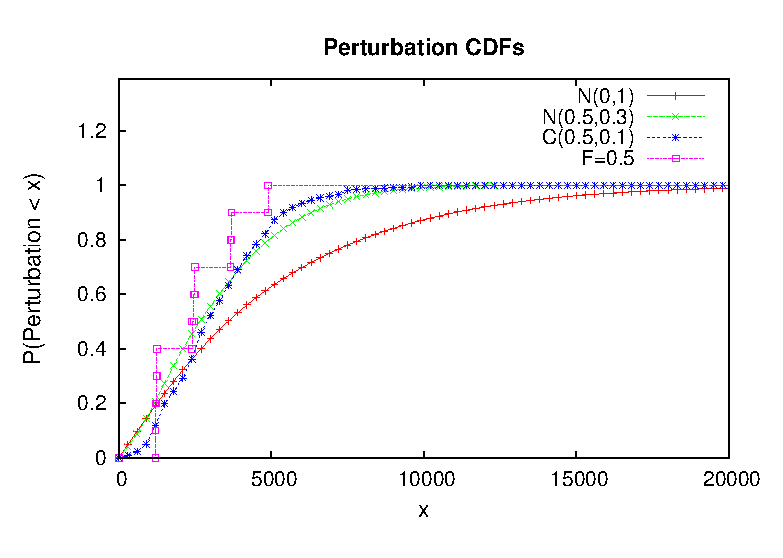
\includegraphics[width=0.40\textwidth]{images/cdf.eps}
\caption{\textsc{cdf}s used for mutating in different \DE{} variants}
\label{fig:random_cdfs}
\end{figure}

\DE{} with the distributions tested tend to yield small perturbations with a larger probability than the basic \DE{}.
%
In fact, the original \DE{} does not yield perturbations smaller than 1,200 units.
%
However, in the rest of the schemes, the probability of producing a perturbation lower than 1,200 units is larger than 12\%.
%
In the same way, larger perturbations than in the original \DE{} might be generated.
%
For instance, \DE{} with fixed $F$ does not produce any perturbation larger than 5000 units.
%
However, the probabilities of having such perturbations with the remaining distributions are not insignificant.
%
Thus, many of the perturbations might generate individuals outside the feasible region.
%
In fact, several perturbations larger than the search space size can be carried out.
%
These undesired movements might deteriorate the performance of \DE{}, especially when dealing with large spaces where the
percentage of space explored by \DE{} is smaller than in low-dimensional spaces.
%
Considering all these properties, it is clear that using such random distributions might have a large impact on the results.
%
However, it is not clear whether these properties are beneficial when high-dimensional spaces are involved.

In other promising schemes, the feedback obtained during the execution is used to set the value of $F$.
%
In these cases, it is not easy to develop a theoretical analysis because the behavior depends on the function to be optimized.
%
However, it is important to note that the advantages of using feedback are not as robust as expected~\cite{Zielinski:08,Segura:14}.
%
In any case, since some state-of-the-art \DE{} schemes use feedback to set the value of $F$,
the experimental evaluation developed in this research takes into account some of the most well-known adaptive schemes.

\section{Our Proposals}
\label{sec:proposal}

In this paper, a novel \DE{} scheme is proposed whose aim is to avoid the aforementioned weaknesses.
%
The scheme incorporates two main modifications.
%
Both proposals change the way of perturbing solutions in \DE{}.
%
Specifically, when the new modifications are considered, the way of calculating the perturbation size is modified.
%
Thus, instead of using the scaled difference vector to perturb a given base vector, alternative
methods are applied.
%
The principle of the first modification is to increase the number of potential trial solutions while at the same
time preserving the basic behavior of \DE{}.
%
The aim of the second modification is to improve the exploration capabilities of \DE{} so as to
correctly deal with large search spaces and enable additional ways of avoiding stagnation
and premature convergence.
%
Both modifications are used when a trial vector that considers only one mutant variable
is going to be created, i.e., when the value $L$ generated by the exponential crossover is equal to one.
%
%Considering the truncated geometric distribution used in the exponential crossover (see~(\ref{eq:geometric_dist})), this happens with a probability equal to
%$(1 - CR) \times 100$, which is large enough to have a significant impact on the final results.
%
These modifications might also be applied when several mutant variables are inherited by the trial vector.
%
This can be done in several ways, however, and requires a more in-depth study considering the relationships
among the distributions that arise for the different variables.
%
\textcolor{red}{
Some initial experimentation by considering the distributions as if they were independent were carried out.
%
However, this resulted in unsuccessful schemes.
%
This could be probably fixed by taking into account the relations among the distributions that arise in the different variables.
%
One option might be to apply copula functions, as it has been done in Estimation of Distribution Algorithms~\cite{Rogelio:09}.
%
However, this would result in a very complex scheme.
%In fact, this is related to the dither and jitter schemes, which is still an open research topic~\cite{Price:13}.
%
Since quite promising results are obtained without the incorporation of such more complex schemes, 
this analysis is beyond the scope of this paper.
}

\subsection{Continuation Scheme}

The aim of the first modification is to increase the number of potential trial vectors that can be generated
with \DE{}.
%
In order to define the proposal, the mathematical analysis developed for the \DE{}
schemes presented before for dealing with random $F$ values was considered.
%
One of the main strengths of these models is that any perturbation between the maximum and the minimum
admissible perturbations has a non-zero probability of being generated.
%
Thus, if for a given variable $i$ the maximum and minimum perturbations that can be generated with a given distribution
are $max_i$ and $min_i$, respectively, any modification in the range [$min_i$, $max_i$] can be generated.
%
In other words, the \textsc{cdf} is monotonically increasing in this range.
%
This does not happen when a fixed value of $F$ is used.
%
In contrast, the main weaknesses detected involve the very small or large mutations that
are occasionally carried out.

%As noted earlier, there are serious doubts concerning the robustness of the schemes based on using feedback to set the $F$ value.
%
%In fact, some schemes that rely on random distributions to set the value of $F$ have yielded quite competitive results~\cite{Zielinski:08},
%meaning that the benefits of these proposals might be provided by the increased diversity.
%
%One of the best behaved \DE{} schemes~\cite{LaTorre:11} in the special issue compiled by \textsc{soco} considered
%a fixed $F$ value and was able to outperform other adaptive schemes.
%
%This scheme is a hybrid method that provides diversity in different ways.
%
%Since in our scheme we are also promoting diversity in a different way,
%and taking into account the previously discussed drawbacks of using adaptive $F$ values,
%in the newly defined proposal a fixed value of $F$ is considered.
%
%Note that this is somewhat related to the \textit{derandomized} evolution strategies~\cite{Ostermeier:94},
%because this process replaces the use of random values by a less stochastic way of promoting diversity.
%
Our proposal is based on generating a monotonically increasing \textsc{cdf} %in the range of accepted perturbations
by slightly modifying the \textsc{cdf}s that appear in those \DE{} schemes that consider a fixed $F$ value.
%
Then, these \textsc{cdf}s are used to generate random numbers that are multiplied
by $F$ and used to mutate the population vectors, just as in the original \DE{}.
%
The scheme functions as follows.
%
First, an approximation of the \textsc{cdf} that models the absolute values
of the perturbation performed by a \DE{} with $F = 1$ is calculated for the variable that is going to be mutated.
%
This is done by considering~(\ref{eq:approx_CDF}), where $minor(x)$ is the number of differences that appear in
the population that are lower than $x$.
%
The denominator is the amount of vector differences appearing in the population minus one.
%
This ensures that the maximum value of~(\ref{eq:approx_CDF}) is one.
%
The generated \textsc{cdf}s have the form of a step function.
%
Then, for each difference ($d$) that does not appear in the current population and that is located between the minimum and maximum
existing differences, $CDF(d)$ is calculated using a linear interpolation.
%
The interpolation is done by considering the differences $d1$ and $d2$, where $d1$ is the highest
difference lower than $d$ that appears in the population, and $d2$ is the lowest difference higher than $d$ that appears in the population.

\begin{equation}
	\label{eq:approx_CDF}
		CDF(x) = {{minor(x)}\over{0.5 \times (NP) \times (NP-1) - 1}}
\end{equation}

As an example, assume that the set of differences
appearing in a given population with $NP = 5$ is: ${1.1, 1.3, 1.4, 1.41, 1.43, 1.45, 8, 8.3, 8.5, 8.7}$.
%
\figurename~\ref{fig:new_CDFs} shows the \textsc{cdf} corresponding to a \DE{} with $F = 1$, the
approximate \textsc{cdf} calculated using the above steps --- function (\ref{eq:approx_CDF}) is evaluated for each of
the differences appearing in the population ---
and
the \textsc{cdf} corresponding to the new model, i.e., the previous one with interpolation.
%
The scheme that considers the use of this new \textsc{cdf} is called Continuous Differential Evolution (\CDE{}),
in reference to the fact that any mutation step in the range [$min_i$, $max_i$] can be generated.
%
As we can see, the \textsc{cdf} in \CDE{} has a larger slope in the zones where a larger number of differences appear
and the values $min_i$ and $max_i$ remain intact.
%
Thus, differently to the cases that apply a variable $F$ value, 
the \DE{} principle that correlates the strength of the mutation to the size of the differences is better respected
in our transformation.
%
At the same time, the number of potential trials is augmented with the aim of avoiding stagnation.

\begin{figure}[!t]
\centering
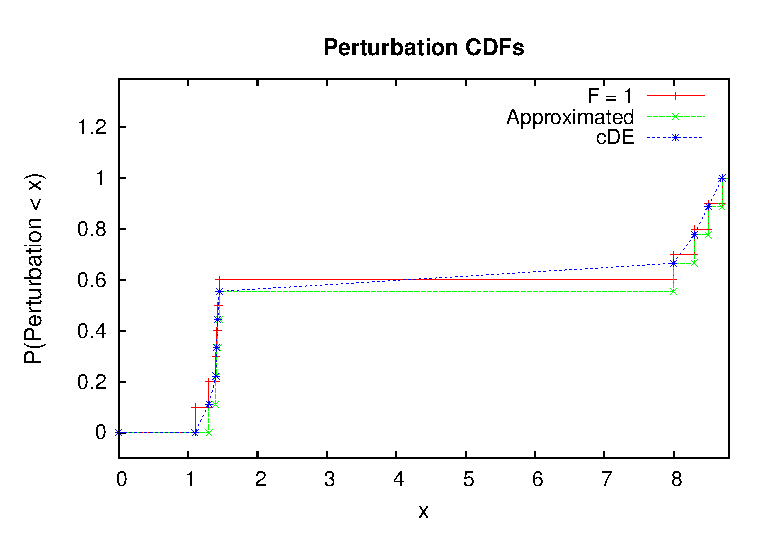
\includegraphics[width=0.40\textwidth]{images/CDFs/cdf_new.eps}
\caption{\textsc{cdf} generated with \CDE{}}
\label{fig:new_CDFs}
\end{figure}

\textcolor{red}{
Note that in order to calculate the \textsc{cdf}, ${{NP \times (NP - 1)}\over{2}}$ distances must be taken into account.
%
In our implementation, the only \textsc{cdf}s that are calculated are the ones that are used in each generation.
%
In the worst case, and taking into account that for large-scale optimization, $NP$ is usually much smaller than $D$, $NP$ \textsc{cdf}s should be calculated,
meaning that in the worst case about $NP^3$ operations are required.
%
However, in the average case less operations are used.
%
In fact, when the ``exp'' crossover is taken into account, in average in each generation only $(1 - CR) \times NP$ \textsc{cdf}s are calculated, meaning
that the time associated to the continuation scheme is shorter.
%
In the case of using benchmark problems, this task can consume a non negligible proportion of the total time.
%
For instance, when \DE{} with $NP = 15$ and $CR = 0.9$ is used to solve the \textsc{f1} problem of the \textsc{soco} benchmark, the model with the continuation
scheme use about 35\% of additional time.
%
Moreover, the penalty grows for larger population sizes.
%
Specifically, the penalty is 75\% when $NP$ is set to 30 and 255\% when $NP$ is set to 50.
%
However, when more expensive functions are used these penalties diminish drastically.
%
Once that a case is analyzed, it is not difficult to predict the penalty obtained for other problems.
%
The most important features are the evaluation time associated to the new problem and the value of $NP$.
%
For instance, if for a given problem whose evaluation cost is $EvCost$, the basic \DE{} variant takes $t1$ seconds to complete $StopEv$ evaluations
and the model that incorporates the continuation scheme takes $t2$ seconds, the penalty percentage can be approximated using~(\ref{eq:approx_penalty}).
%
In such an equation, $t$ represents the evaluation time associated to the problem whose penalty is predicted.
}
%

\begin{equation}
	\label{eq:approx_penalty}
		Penalty(t) = {{t2-t1}\over{t1 -StopEv \times EvCost + StopEV \times t}} \times 100
\end{equation}

\textcolor{red}{
Figure~\ref{fig:time} shows an approximation of the penalty by using the data obtained for \textsc{f1} with three different values of $NP$.
%
We can appreciate that for short evaluation times the penalty is large.
%
However, as the evaluation time increases, the penalty quickly diminishes.
%
In order to evaluate the accuracy of the approximation, the penalties associated to \textsc{f17} were calculated.
%
Experimentally, the penalties were 0.87\%, 2.02\% and 4.3\% when $NP$ was set to 15, 30 and 60, respectively.
%
In the \textsc{f17} problem, the evaluation takes about $3 \times 10^{-4}$ seconds, so the predicted values are
0.42\%, 0.87\% and 2.93\%.
%
While these values are not exact, they are proper approximations, so (\ref{eq:approx_penalty}) can be used to accurately estimate the penalties.
%
Anyway, the key is that even with relatively inexpensive evaluation functions as \textsc{f17}, the penalty is not too large, so
in computationally demanding problems the penalty term is probably negligible.
%
For this reason, in this work the computational study has been done taking into account the number of evaluations instead of the time.
}

\begin{figure}[!t]
\centering
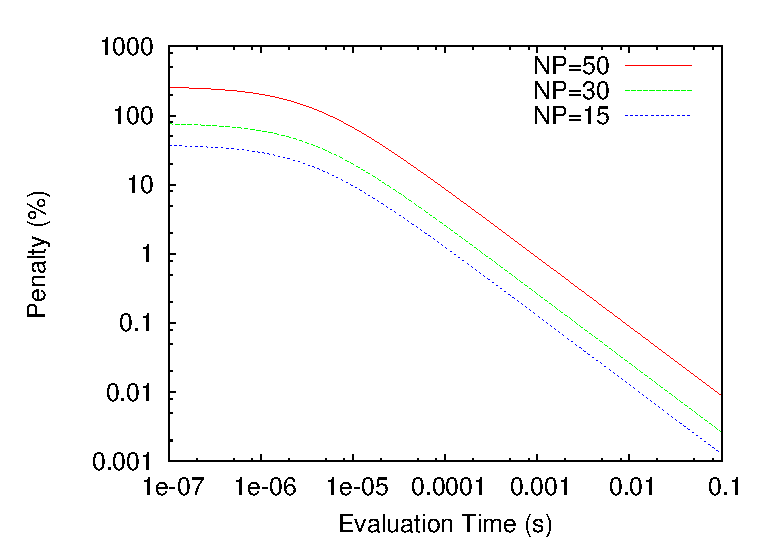
\includegraphics[width=0.40\textwidth]{images/Time/timePrediction.eps}
\caption{Approximation of the penalty (\%) induced by the continuation scheme}
\label{fig:time}
\end{figure}

\subsection{Avoiding a Large Reduction in Diversity}


Initial experimentation ---which did not consider any technique to promote large perturbations---
has shown that large mutations were not required in most of the executions.
%
However, in some of the worst cases, the maximum difference between the values appearing for one variable might be
highly reduced from one generation to the next.
%
This might leave large portions of the search space unexplored, yielding unsatisfactory results.
%
In addition, our initial experiments showed that the likelihood of this occurrence increases with the
number of dimensions considered.
%
Our analysis showed that this was related to the \textit{fake large} moves studied in~\cite{Montgomery:09},
which are a set of moves that appears when there are some low differences in the population.
%
Note that, given two randomly generated individuals ($X_i$ and $X_j$), the probability ($P$) that the difference between the values
of their corresponding $v$-th variables will be lower than $\epsilon$ is given by~(\ref{eq:prob_dif_lower_eps}).
%
Obviously, as the number of dimensions considered grows, the probability associated with the appearance of low differences in at least one variable
increases sharply.
%
Specifically, the expected number of variables where this happens is $D \times P$, meaning that as the number of dimensions
grows, there will be a larger number of variables where low differences will appear.
%
In fact, the probability associated to this event tends to one when the number of variables considered tends to infinity.

\begin{equation}
	\label{eq:prob_dif_lower_eps}
		P(|x_{i,v} - x_{j,v}| < \epsilon) = {{2 \epsilon}\over{b_v - a_v}} - {{\epsilon^2}\over{({b_v - a_v})^2}}
\end{equation}
%

The previous formula applies to any variant of \EAS{}.
%
However, \DE{} is the only variant which is affected by the \textit{fake large} moves, which is why special actions
must be taken in \DE{}.
%
Considering this and the promising results that have been obtained with complex multimodal problems by using distributions with long tails to generate the $F$ values~\cite{Price:13},
we decided to design an adaptive scheme
that promotes large perturbations in a controlled fashion.
%
Since the scheme promotes large perturbations, using it frequently might provoke a too disruptive scheme.
%
For this reason, the scheme is only used when the value $L$ generated by the exponential crossover is equal to one
and with a ratio equal to \HMR{} --- high mutation ratio.
%
In the remaining cases (ratio $1 - $\HMR{}), the original \DE{} or the continuation scheme previously described is applied.

The scheme operates as follows.
%
Each time that it is applied to a given variable $i$, a large random number ($R$) is generated.
%
Then, $R$ is used to perturb such a variable in the base vector, i.e., it acts as the scaled difference vector in the original \DE{}.
%
In half of the cases it is added and in the remaining cases it is subtracted.
%
In order to calculate $R$, our scheme stores the maximum admissible mutation ($FalseMax_i$) for each variable $i$.
%
Initially, they are set using~(\ref{eq:max_mut}).
%
Thus, a maximum $R$ equal to at least 20\% of the variable range size is initially allowed.
%
Then, $R$ is generated by producing a random number in the range $[Max_i, FalseMax_i]$, 
where $Max_i$ represents the maximum perturbation that can be generated for such a variable by using the \textsc{cdf} of \CDE{}.
%
\textcolor{red}{
In every generation, if the value of $FalseMax_i$ is higher than $Max_i$, $FalseMax_i$ is reset to $Max_i$.
%
This usually happens in the first generation, meaning that our scheme is not sensitive to the initialization of $FalseMax_i$.
%
Anyway, it is adequate to maintain this initialization in order to ensure a minimum amount of perturbation, even if
an improper initial population is generated.
}
%
After perturbing the base vector, the value $FalseMax_i$ is updated.
%
In cases where the trial vector generated was successful, i.e., better than the target vector,
the value is updated with~(\ref{eq:update_max_sum}).
%
Otherwise, it is updated with~(\ref{eq:update_max_substract}).
%
The principle of the update mechanism is 
similar to the one that governed the design of the Win or Learn Fast approach~\cite{Bowling:01}.
%
Specifically, in the cases where large mutations are successful, even larger mutations
are promoted.
%
In contrast, when mutations are not successful, the maximum admissible mutation for this variable is shortened.
%
\textcolor{red}{
The $UpdateDenom$ parameter can be used to set the velocity of adaptation of $FalseMax_i$.
%
Specifically, when larger values are used, a slower adaptation is done.
%
As a result, higher values should be used for cases where a higher balance towards exploration is required.
%
Note that the denominators in (\ref{eq:update_max_sum}) and (\ref{eq:update_max_substract}) might even take different values among them.
%
However, since the experimental evaluation shows that the new proposal is not too sensitive to this parameter, dedicating many
efforts to tune the update mechanism in this way seems not very promising.
}

\begin{equation}
	\label{eq:max_mut}
		FalseMax_i = {{b_i - a_i}\over{5}}
\end{equation}

\begin{equation}
	\label{eq:update_max_sum}
		FalseMax_i = FalseMax_i + {{(FalseMax_i - Max_i)}\over{UpdateDenom}}
\end{equation}

\begin{equation}
	\label{eq:update_max_substract}
		FalseMax_i = FalseMax_i - {{(FalseMax_i - Max_i)}\over{UpdateDenom}}
\end{equation}

%
%It is also important to note that the maximum initial perturbation, as well as the way in which $FalseMax_i$ is updated, can be done in several different ways.
%
%For instance, if larger perturbations are desired, the initial perturbation might be set to a larger value or the updating mechanisms
%might by slowed down by using larger denominators in (\ref{eq:update_max_sum}) and (\ref{eq:update_max_substract}).
%
%In fact, the denominators in (\ref{eq:update_max_sum}) and (\ref{eq:update_max_substract}) might even take different values among them.
%
%Parameter setting strategies~\cite{Lobo:07} might also be used to optimize the scheme even further.
%
%In this paper we consider them as fixed attributes, i.e., every experiment considers the specific values given before.
%
%These specific values were set by considering some preliminary executions.
%
%Since several components are already involved, it is beyond the scope of this research to engage in detailed studies on the effects of these parameters.

\textcolor{red}{
Finally, we would like to mention that considering that the schemes that adapt the $F$ value usually improve on the intensification capabilities of \DE{},
incorporating some modifications to enhance the exploitation features of \DE{} seems promising.
%
In fact, some of the most promising schemes published in the
literature are hybrid approaches that combine \DE{} with local search mechanisms~\cite{LaTorre:14}.
%
As it has been mentioned, in some of the most promising hybrid schemes, as \textsc{mos}~\cite{LaTorre:11}, several components are used to do global search.
%
We did some initial tests by incorporating a local search mechanism at the end of the executions. 
%
However, these schemes were not as successful as other hybrid approaches were several components are in charge of the global search.
%
This means that while our schemes clearly improve the global search capabilities --- as it is shown with the experimental validation---, 
additional efforts are required prior to being able of developing
a competitive \DE{} for large-scale optimization where no other components to do global search are taken into account.
%
Thus, improving further the global search capabilities as well as 
hybridizing the new \DE{} schemes with some of the highly efficient local search mechanisms proposed
in the literature, is left for future work.
}

\section{Experimental Evaluation}
\label{sec:exp}

In this section, the experiments conducted with the newly designed \DE{} scheme are described.
%
%The optimization schemes were implemented using \METCO{}
%(\emph{Metaheuristic-based Extensible Tool for Cooperative Optimization})~\cite{Leon:09}.
%
Most of the analyses were performed with the
benchmark problems devised for \textsc{soco}~\cite{Lozano:10}, which are a
set of 19 scalable continuous optimization problems to be minimized.
%
The parameter $D$ allows setting the number of variables in the problems.
%
These problems have different features and combine different properties
involving modality, separability, and ease of optimization dimension by dimension.
%
In order to analyze the schemes, six sets of experiments were carried out with such a benchmark.
%
In every case,
each execution was repeated 1000 times, unless otherwise stated.
%
In addition, and so as to illustrate how our schemes can provide benefits for problems with very different features,
we also conducted some experiments with the \textsc{cec'10} test problems~\cite{Tang:10}.
%
As previously described, the schemes that have reported promising results for each of these benchmarks are quite different.
%
Specifically, the selection of the proper crossover operator seems very important.
%
In the case of the \textsc{soco} test problems, and considering the results obtained in~\cite{LaTorre:11},
exp crossover was used.
%
In the case of the \textsc{cec} test problems,  similarly to the scheme devised in~\cite{Brest:10}, in our proposal we decided to
alternate between the use of bin and exp crossover operators,
using the bin operator in even generations and the exp operator
in the odd ones.
%
The other properties of \DE{} were the same for both benchmarks.

Since stochastic algorithms were considered in this study, comparisons were carried out by applying a set of statistical tests.
%
A similar guideline as the one applied in~\cite{Durillo:10} was taken into account.
%
Specifically, the following tests were applied, assuming a significance level of 5\%.
%
First, a \emph{Shapiro-Wilk test} was performed to check whether or not
the values of the results followed a Gaussian distribution.
%
If so, the \emph{Levene test} was used to check for the homogeneity of the variances.
%
If samples had equal variance, an \emph{\textsc{anova} test} was done; if not, a \emph{Welch test} was performed.
%
For non-Gaussian distributions, the non-parametric \emph{Kruskal-Wallis} test was
used for testing whether samples are drawn from the same distribution.
%
Note that some researchers~\cite{Good:92} have suggested that the obtained p-values might be normalized 
by taking into account the number of independent executions carried out.
%
However, in our experiments the p-values were either very high or very low, so such scaling does not
affect the results of our statistical tests.
%
In this work, the sentence ``algorithm A is better than algorithm B'' means that the
differences between them are statistically significant, and that the mean and median obtained
by A are lower ---one of the metrics might be equal--- than the mean and median achieved by B.
%
\textcolor{red}{
In the experiments below, the tables provided show the results of certain statistical tests used to
compare a variant of \DE{} with the same scheme, but incorporating our proposals.
%
In these tables the following symbols, and their associated meanings, are used:
%
\begin{itemize}
	\item $\uparrow$: the model that incorporates our proposals is better.
	\item $\downarrow$: the model that incorporates our proposals is worse.
	\item $*$: differences are statistically significant, and the model that incorporates our proposals achieves a higher mean and lower median.
	\item $**$: differences are statistically significant, and the model that incorporates our proposals  achieves a lower mean and higher median.
	\item $\leftrightarrow$: differences are not statistically significant.
\end{itemize}
%
}

\subsection{First Set of Experiments: Benefits of each Proposal}

As described in Section~\ref{sec:proposal}, in this work we propose two modifications for enhancing \DE{}.
%
Each modification can be included separately into \DE{} or they can be used in conjunction.
%
The aim of the first experiment was to analyze the benefits contributed by each proposal.
%
The \DE{} schemes that incorporate the continuation scheme are referred to as \CDE{}, whereas in those cases where it
was not considered, the term \DE{} is used.
%
\textcolor{red}{
Regarding the scheme that promotes the use of large perturbations, the $UpdateDenom$ parameter was set to 10 and
several \HMR{} ratios were considered.
}
%
Specifically, the following ratios were tested: 0, 0.01, 0.02, 0.04, 0.08, 0.16, 0.32 and 0.64.
%
In the rest of the paper, the models are referred to as \DE{}-\HMR{} or \CDE{}-\HMR{}.
%
If no value for \HMR{} is given, it means that \HMR{} $ = 0$ is assumed.
%
The number of variables $D$ was fixed to 50 in a first set of experiments,
while the stopping criterion was set to 150$\,$000 function evaluations.
%
Both \DE{} and \CDE{} were parameterized as in~\cite{LaTorre:11}.
%
Specifically, the vector generation strategy used was DE/rand/1/exp, while
$F$ and $CR$ were set to 0.5.
%
Finally, \NP{} was set to 15.

\begin{figure*}[!t]
\centering
\begin{tabular}{ccc}
  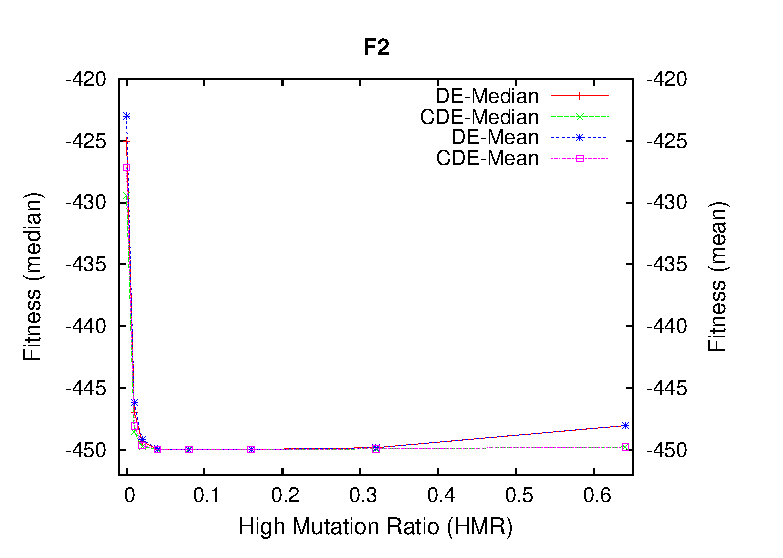
\includegraphics[width=0.32\textwidth]{images/HighMutRatio_150000/F2_50_HighMutRatio.eps} & 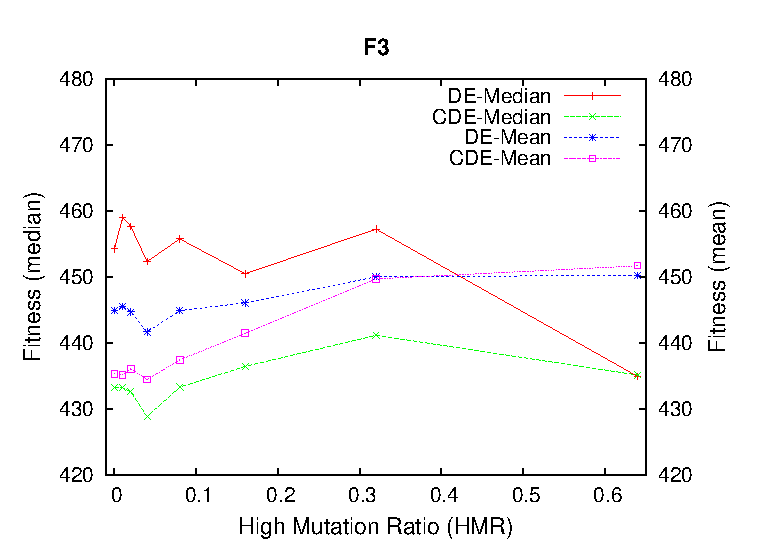
\includegraphics[width=0.32\textwidth]{images/HighMutRatio_150000/F3_50_HighMutRatio} & 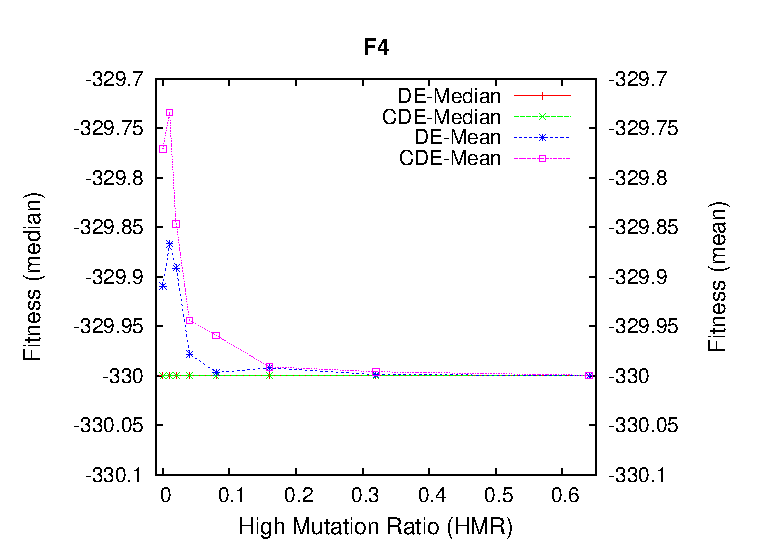
\includegraphics[width=0.32\textwidth]{images/HighMutRatio_150000/F4_50_HighMutRatio} \\
  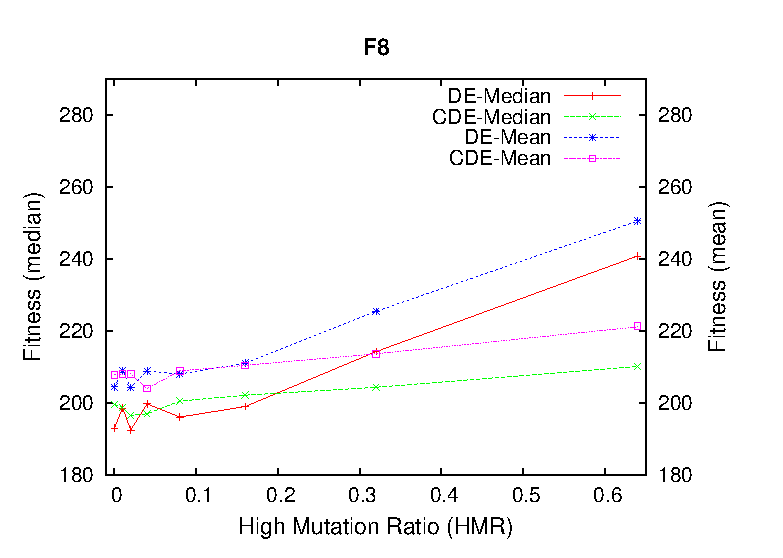
\includegraphics[width=0.32\textwidth]{images/HighMutRatio_150000/F8_50_HighMutRatio} & 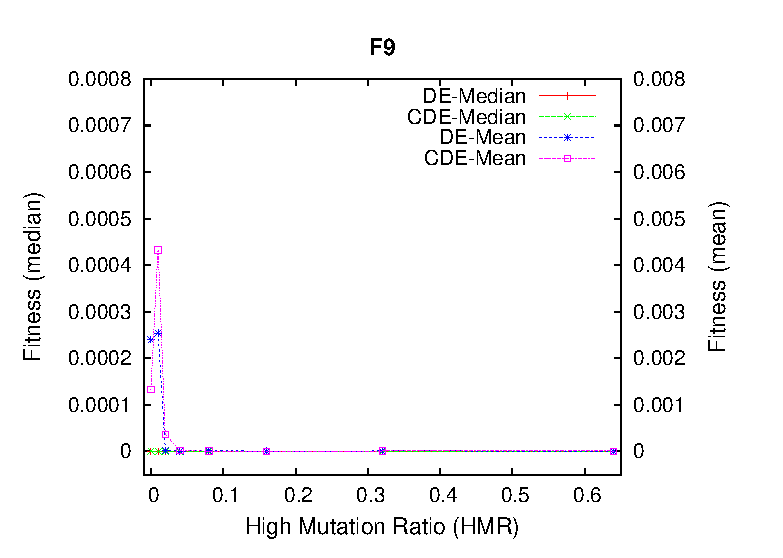
\includegraphics[width=0.32\textwidth]{images/HighMutRatio_150000/F9_50_HighMutRatio} & 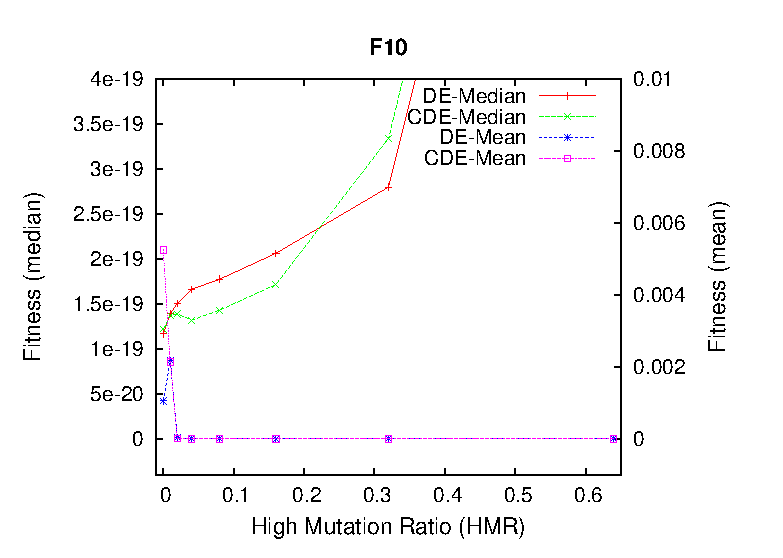
\includegraphics[width=0.32\textwidth]{images/HighMutRatio_150000/F10_50_HighMutRatio} \\ \\
  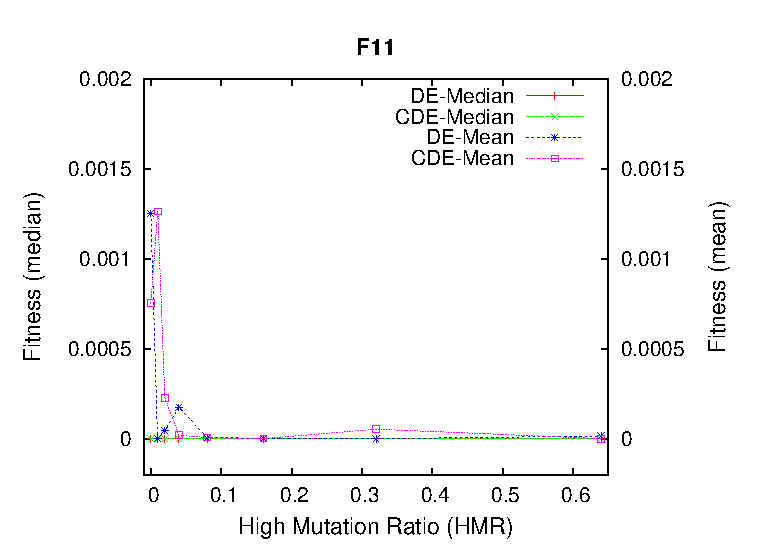
\includegraphics[width=0.32\textwidth]{images/HighMutRatio_150000/F11_50_HighMutRatio} & 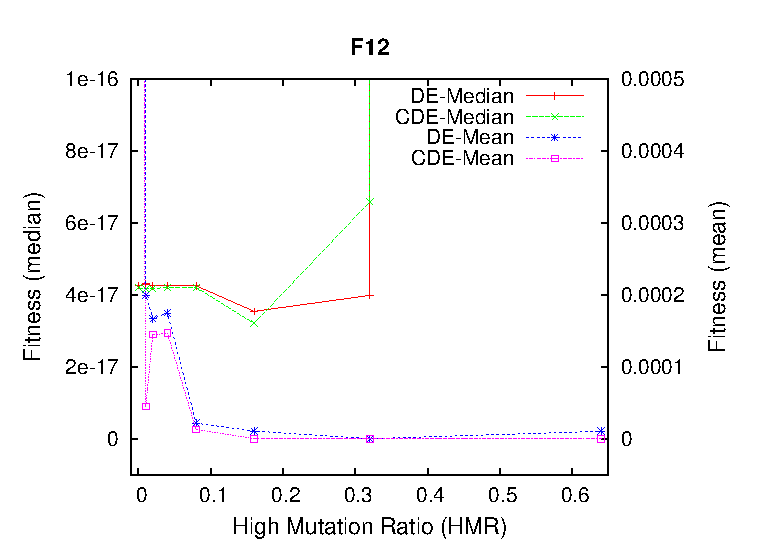
\includegraphics[width=0.32\textwidth]{images/HighMutRatio_150000/F12_50_HighMutRatio} & 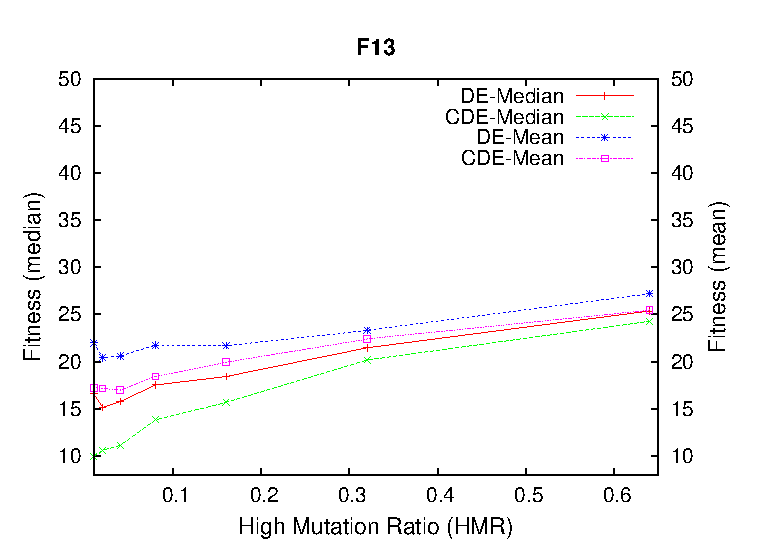
\includegraphics[width=0.32\textwidth]{images/HighMutRatio_150000/F13_50_HighMutRatio} \\
  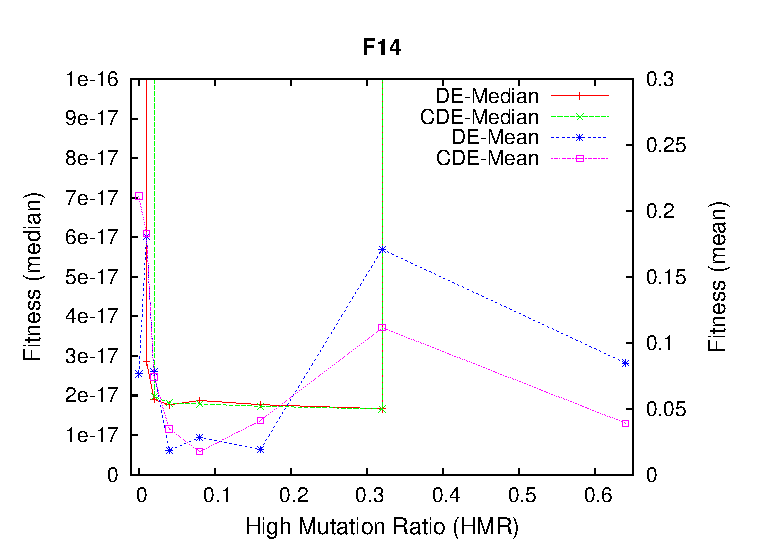
\includegraphics[width=0.32\textwidth]{images/HighMutRatio_150000/F14_50_HighMutRatio} & 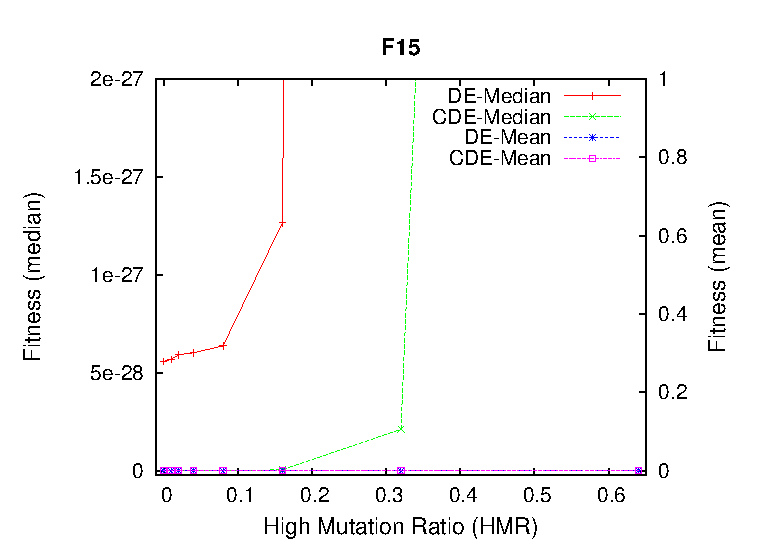
\includegraphics[width=0.32\textwidth]{images/HighMutRatio_150000/F15_50_HighMutRatio} & 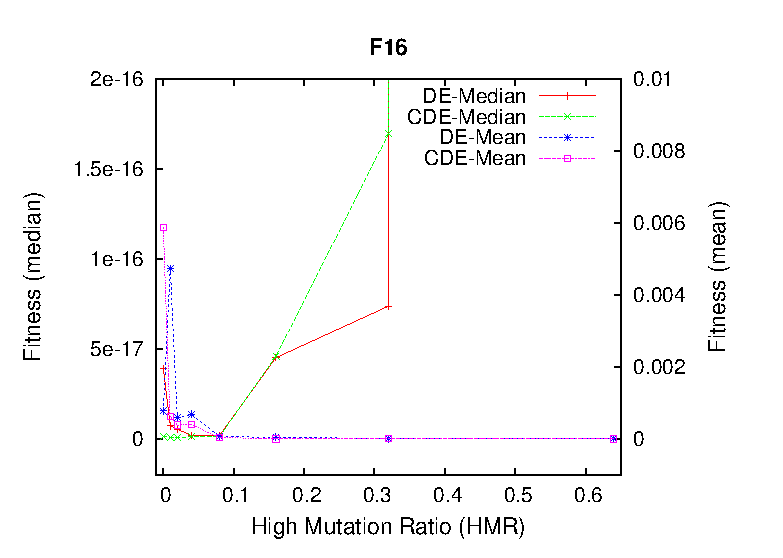
\includegraphics[width=0.32\textwidth]{images/HighMutRatio_150000/F16_50_HighMutRatio} \\ \\
  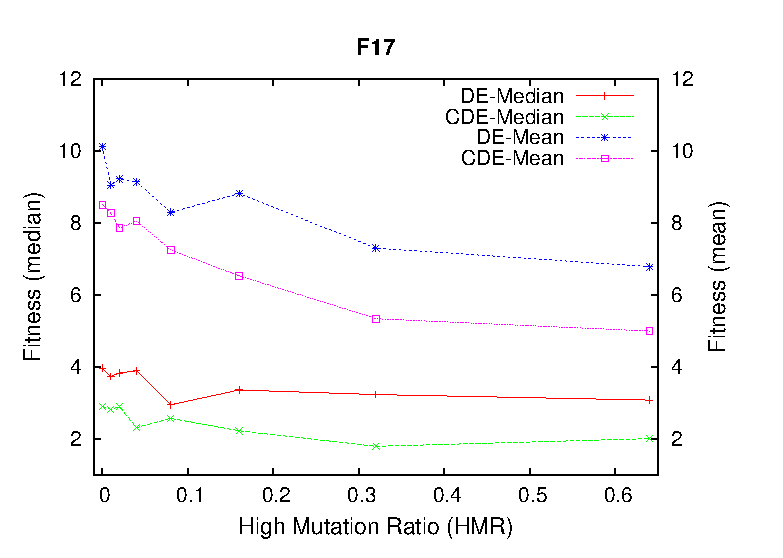
\includegraphics[width=0.32\textwidth]{images/HighMutRatio_150000/F17_50_HighMutRatio} & 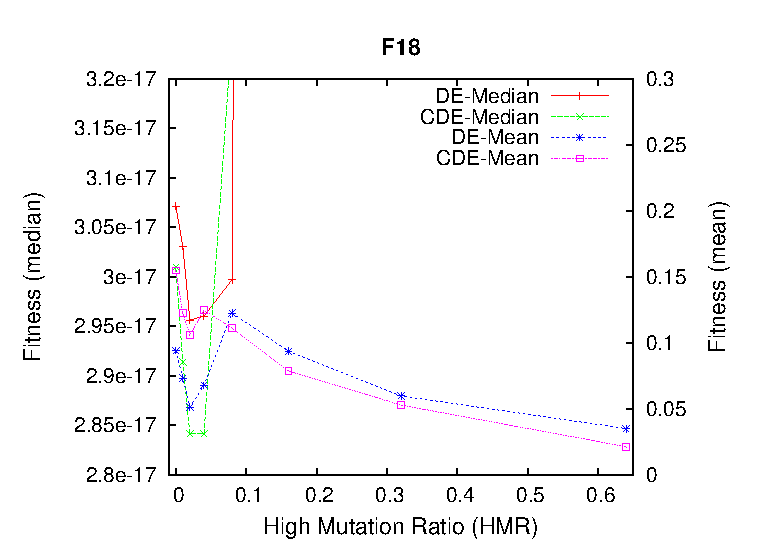
\includegraphics[width=0.32\textwidth]{images/HighMutRatio_150000/F18_50_HighMutRatio} & 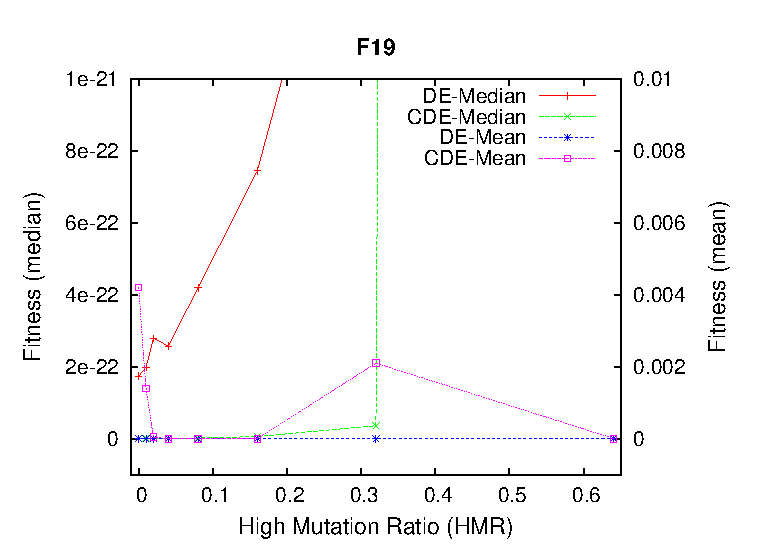
\includegraphics[width=0.32\textwidth]{images/HighMutRatio_150000/F19_50_HighMutRatio} \\ 
\end{tabular}
\caption{Mean and median obtained by \DE{} and \CDE{} with different values of \HMR{} in 150$\,$000 function evaluations for several functions}
\label{fig:exp1_1}
\end{figure*}



\figurename~\ref{fig:exp1_1} shows the median and mean values obtained with the different schemes at the end of the executions for the set of functions
where the new schemes caused a larger effect on the results.
%
Specifically, they show the results for \DE{} and \CDE{} with the different values of \HMR{}.
%
Since in some functions the means and medians obtained were quite different, different axes are used
to represent each of them.
%
In most of the problems tested, the positive effect of considering
an \HMR{} value different from 0 is clear, both for \DE{} and \CDE{}.
%
The effects caused by the low values of \HMR{} on the mean are more significant than on the median.
%
The reason is that in most of the problems, premature convergence only appears occasionally, so the large perturbations resulting from
the use of a non-zero \HMR{} have the main effect of improving the worst-case behavior, which significantly reduces the mean but not the median.
%
For instance, some cases where this effect is clear are F4 and F9, where even large \HMR{} values can be successfully applied.
%
However, in F13 and F15, making large perturbations does not provide benefits, probably because these problems are not as heavily affected by premature convergence.
%
Also worth noting is the fact that there are some problems, e.g., F4 and F17, where the best results are obtained by considering very high \HMR{}
values.
%
This indicates that a large loss of diversity is emerging in these problems, so using large perturbations frequently is helpful.
%
However, in most of the test cases, using a too high value for \HMR{} deteriorates the quality of the results
because the scheme loses its intensification capabilities.
%
Some cases where this happens are F10, F12, F14 and F15.
%
Note than in these last problems, the medians are much lower than the mean values.
%
This happens in several problems where the eventual executions that suffer from premature convergence govern the resulting mean value.
%
In these cases, using a large \HMR{} does not significantly deteriorate the mean value, at least when compared to the deterioration
caused by the use of \HMR{} = 0.
%
The reason is that as \HMR{} increases, the likelihood of premature convergence does not increase.
%
However, since many large perturbations are involved, the typical executions are affected, meaning that the medians are more heavily penalized.
%
Considering the overall results, the most promising schemes consider low, but non-zero, values of \HMR{}; specifically, the \CDE{} scheme, where \HMR{} $ = 0.04$ seems very promising.

\begin{figure}[!t]
\centering
\begin{tabular}{cc}
  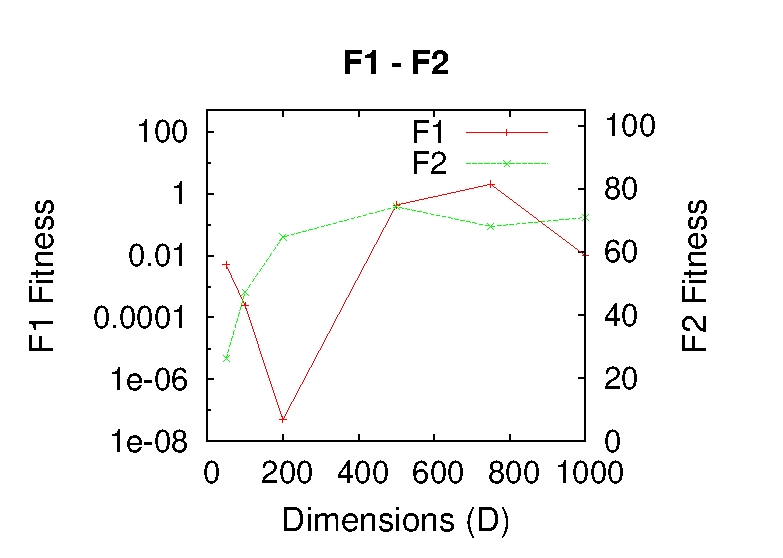
\includegraphics[width=0.36\textwidth]{images/DifGrow/F1_F2_DifGrow.eps} & 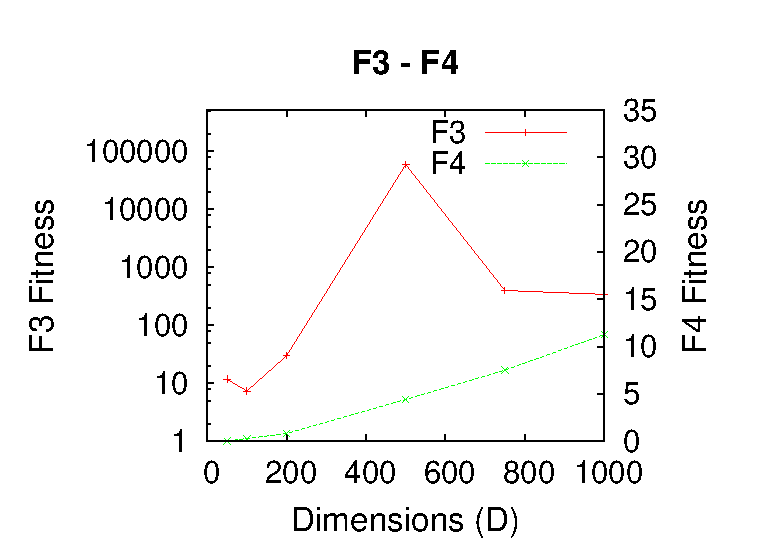
\includegraphics[width=0.36\textwidth]{images/DifGrow/F3_F4_DifGrow.eps}
\end{tabular}
\caption{Differences between the maximum and minimum obtained means with different \HMR{} values for several functions}
\label{fig:hmr_dimensions}
\end{figure}


It is also remarkable that in several cases, the differences between the errors obtained by using different \HMR{} values are not too large.
%
This happens because relatively low errors are obtained for several of the functions with low dimensionalities.
%
\DE{} was executed with the previously tested \HMR{} values for the following values of $D$: 50, 100, 200, 500 and 1000.
%
The stopping criterion was set at $5000D$ in every case.
%
\figurename~\ref{fig:hmr_dimensions} shows, for the first four problems, the differences between the maximum and minimum mean fitness values
obtained by using the different \HMR{}.
%
It is quite clear that as the dimensionality grows, the effect of \HMR{} is larger.
%
However, probably due to the stochastic nature of the schemes, the graphics are not monotonically increasing.
%
For instance, in the case of F3, when $D = 500$ was considered, \DE{}-0 exhibited quite a large mean error because
one execution attained a very low quality.
%
Such a high error did not appear when considering larger dimensions, which is the reason why the differences between the
maximum and minimum mean values decreased for these larger dimensionalities.
%
However, in general, larger dimensions imply larger differences.
%
In fact, in every problem the differences that appear for $D = 1000$ are larger
than those that appear for $D = 50$.
%
Several aspects regarding the scalability are analyzed further in subsequent sections.




%\begin{figure*}[!t]
%\centering
%\begin{tabular}{ccc}
%  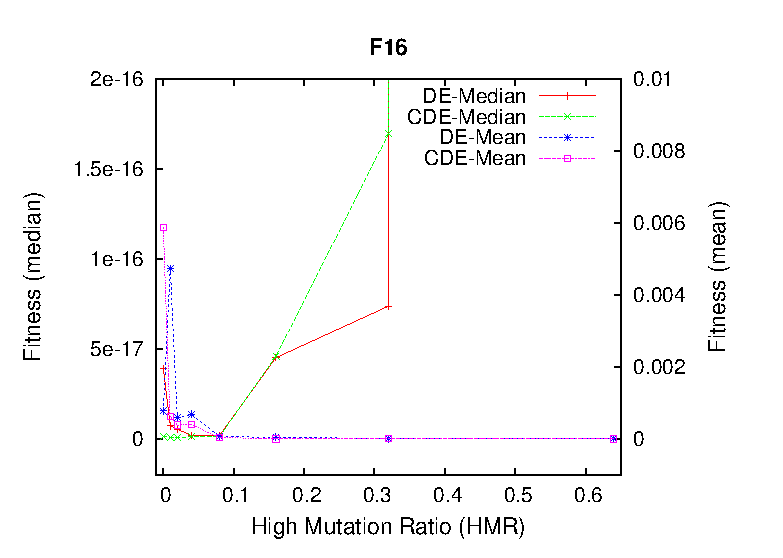
\includegraphics[width=0.32\textwidth]{images/HighMutRatio_150000/F16_50_HighMutRatio.eps} & 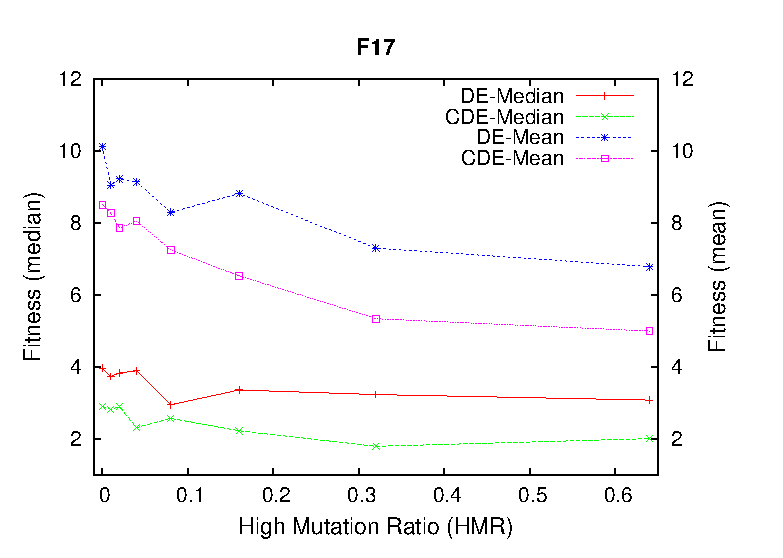
\includegraphics[width=0.32\textwidth]{images/HighMutRatio_150000/F17_50_HighMutRatio} \\
%  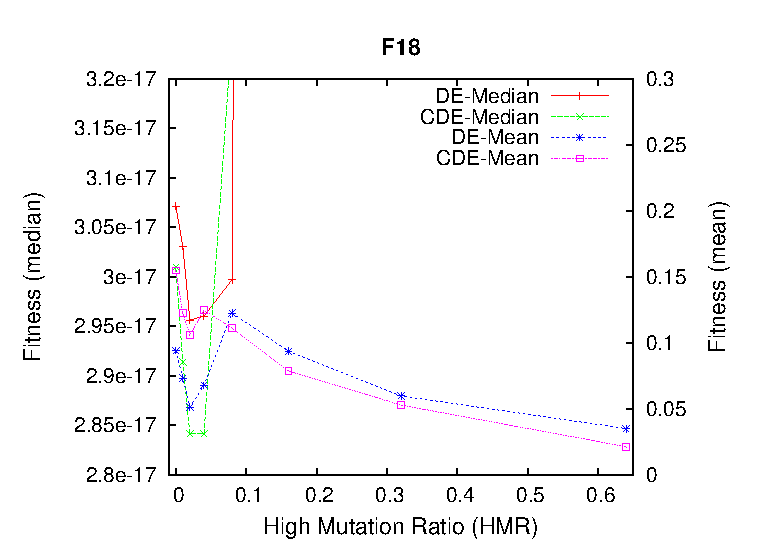
\includegraphics[width=0.32\textwidth]{images/HighMutRatio_150000/F18_50_HighMutRatio} & 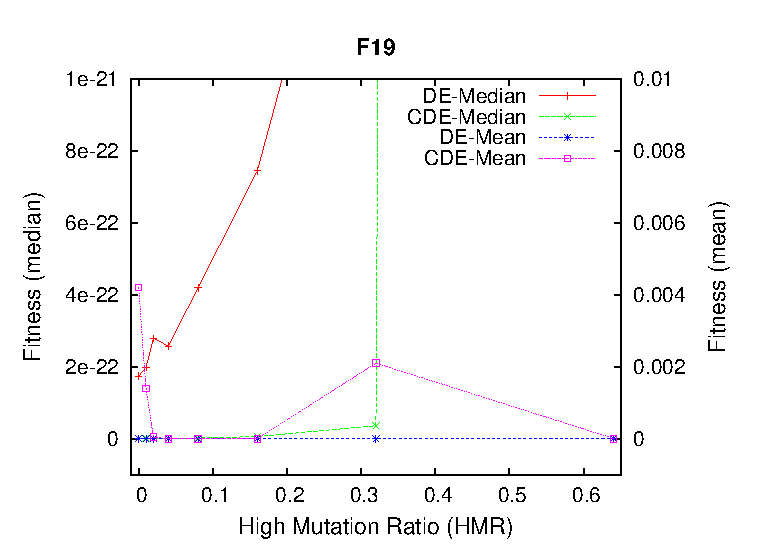
\includegraphics[width=0.32\textwidth]{images/HighMutRatio_150000/F19_50_HighMutRatio}  \\
%\end{tabular}
%\caption{Mean and median obtained by \DE{} and \CDE{} with different values of \HMR{} in 150$\,$000 function evaluations (F16 - F19)}
%\label{fig:exp1_2}
%\end{figure*}

Further statistical analyses were carried out in order to check the benefits of \CDE{} over \DE{}.
%
Specifically, we statistically compared the results obtained by \DE{} and \CDE{} for each value of \HMR{} with $D = 50$.
%
Table~\ref{tab:de_vs_cde_stats} shows the results of these statistical tests.
%
From a total set of 152 statistical tests, \CDE{} is better in 65, while it is worse in only 12, demonstrating its overall superiority.
%
The only problem where \DE{} is clearly superior to \CDE{} is F4.
%
In this case, the optimum values are almost equidistributed in the search space.
%
Thus, \DE{} with an $F$ value equal to 0.5 allows for perturbations that
jump from one local optimum to another local optimum with a large probability.
%
This property is not shared by \CDE{}, which explains its inferior behavior.

\begin{table}[!t]
%\renewcommand{\arraystretch}{1.3}
\caption{Statistical comparison of \textsc{de} vs. \textsc{cde} in 150.000 evaluations}
\label{tab:de_vs_cde_stats}
\centering
\begin{scriptsize}
\begin{tabular}{c c c c c c c c c}
\hline
     & \textsc{hmr} = 0  & \textsc{hmr}= 0.01 & \textsc{hmr}= 0.02 & \textsc{hmr}= 0.04 & \textsc{hmr}= 0.08 & \textsc{hmr}= 0.16 & \textsc{hmr}= 0.32 & \textsc{hmr}= 0.64 \\ \hline
F1	 & $\leftrightarrow$ & $\leftrightarrow$  & $\leftrightarrow$  & $\leftrightarrow$  & $\leftrightarrow$  & $\leftrightarrow$  & $\leftrightarrow$  & $\leftrightarrow$ \\ \hline 
F2	 & $\uparrow$        & $\uparrow$         & $\uparrow$         & $\uparrow$         & $\downarrow$       & $\downarrow$       & $\uparrow$         & $\uparrow$ \\ \hline 
F3	 & $\uparrow$        & $\uparrow$         & $\uparrow$         & $\uparrow$         & $\uparrow$         & $\uparrow$         & $\leftrightarrow$  & $\leftrightarrow$ \\ \hline 
F4	 & $\downarrow$      & $\downarrow$       & $\downarrow$       & $\downarrow$       &  $\downarrow$      & $\leftrightarrow$  & $\leftrightarrow$  & $\leftrightarrow$ \\ \hline 
F5	 & $\leftrightarrow$ & $\leftrightarrow$  & $\leftrightarrow$  & $\leftrightarrow$  & $\leftrightarrow$  & $\leftrightarrow$  & $\leftrightarrow$  & $\leftrightarrow$ \\ \hline 
F6	 & $\uparrow$        & $\uparrow$         & $\leftrightarrow$  & $\leftrightarrow$  & $\leftrightarrow$  & $\leftrightarrow$  & $\leftrightarrow$  & $\leftrightarrow$ \\ \hline 
F7	 & $\leftrightarrow$ & $\leftrightarrow$  & $\leftrightarrow$  & $\leftrightarrow$  & $\leftrightarrow$  & $\leftrightarrow$  & $\uparrow$         & $\leftrightarrow$ \\ \hline 
F8	 & $\leftrightarrow$ & $\leftrightarrow$  & $\leftrightarrow$  & $\leftrightarrow$  & $\leftrightarrow$  & $\leftrightarrow$  & $\uparrow$         & $\uparrow$ \\ \hline 
F9	 & $\uparrow$        & $\leftrightarrow$  & $\leftrightarrow$  & $\leftrightarrow$  & $\uparrow$         & $\uparrow$         & $\uparrow$         & $\leftrightarrow$ \\ \hline 
F10	 & $\leftrightarrow$ & $\leftrightarrow$  & $\uparrow$         & $\uparrow$         & $\uparrow$         & $\uparrow$         & $\downarrow$       & $\downarrow$ \\ \hline 
F11	 & $\leftrightarrow$ & $\leftrightarrow$  & $\leftrightarrow$  & $\leftrightarrow$  & $\uparrow$         & $\uparrow$         & $\leftrightarrow$  & $\leftrightarrow$ \\ \hline 
F12	 & $\uparrow$        & $\uparrow$         & $\uparrow$         & $\uparrow$         & $\uparrow$         & $\uparrow$         & $\downarrow$       & $\uparrow$ \\ \hline 
F13	 & $\uparrow$        & $\uparrow$         & $\uparrow$         & $\uparrow$         & $\uparrow$         & $\uparrow$         & $\leftrightarrow$  & $\uparrow$ \\ \hline 
F14	 & $\downarrow$      & $\leftrightarrow$  & $\leftrightarrow$  & $\leftrightarrow$  & $\leftrightarrow$  & $\leftrightarrow$  & $\leftrightarrow$  & $\uparrow$ \\ \hline 
F15	 & $\uparrow$        & *                  & $\uparrow$         & $\uparrow$         & $\uparrow$         & $\uparrow$         & $\uparrow$         & $\uparrow$ \\ \hline 
F16	 & $\leftrightarrow$ & $\uparrow$         & $\uparrow$         & $\leftrightarrow$  & $\leftrightarrow$  & **                 & $\downarrow$       & $\uparrow$ \\ \hline 
F17	 & $\uparrow$        & $\uparrow$         & $\uparrow$         & $\uparrow$         & $\uparrow$         & $\uparrow$         & $\uparrow$         & $\uparrow$ \\ \hline 
F18	 & $\leftrightarrow$ & $\leftrightarrow$  & $\leftrightarrow$  & $\leftrightarrow$  & **                 & **                 & **                 & $\uparrow$ \\ \hline 
F19	 & *                 & *                  & *                  & $\uparrow$         & $\uparrow$         & $\uparrow$         & *                  & $\uparrow$ \\ \hline 
\end{tabular}
\end{scriptsize}
\end{table}


It is also interesting to perform a statistical comparison of \CDE{}-0.04 with the original \DE{}, i.e., \DE{} with \HMR{} $ = 0$.
%
Table~\ref{tab:de_vs_cde004_stats} shows the results of these comparisons
for a short-time period (75$\,$000 function evaluations) and a longer period (150$\,$000 function evaluations).
%
Even when the differences have been significant, there are some cases where similar medians have been obtained.
%
This has occurred when both schemes have reached the optimal values in most cases.
%
In the case of the median, the symbol $\uparrow$= expresses that differences have been significant and that \CDE{}-0.04 obtained
a lower or similar median than the original \DE{}.
%
Similarly, $\downarrow$= indicates that the original \DE{} obtained a lower or similar median than \CDE{}-0.04.
%
It is interesting to note that:

\begin{itemize}
	\item In the long term, \CDE{} is not statistically inferior in any of the problems, when considering both the mean and median.
	\item In the long term, \CDE{} is superior to \DE{} in 12 problems.
	\item In some of the problems (F4, F7), there are significant differences
       in the short term but both schemes are similar in the long term. The reason is that
       both schemes reach optimal values in most of the executions for these problems in the long term.
	\item In four problems (F9, F11, F12, F16), \CDE{} obtains a lower mean but a higher median
     in the short term, while in the long term, \CDE{} is a better scheme.
\end{itemize}

\begin{figure}[t]
\centering
	\includegraphics[width=0.40\textwidth]{images/cde004_vs_de_boxplots/F9.eps}
\caption{Boxplots of results obtained by \DE{} and \CDE{}-0.04 for different numbers of function evaluations (F9)}
\label{fig:boxplot_cde004_vs_de_f9}
\end{figure}

\begin{table}[!t]
%\renewcommand{\arraystretch}{1.4}
\caption{Statistical comparison of \textsc{de} vs. \textsc{cde}-0.04}
\label{tab:de_vs_cde004_stats}
\centering
\begin{scriptsize}
\begin{tabular}{c c || c | c}
\hline
Median       & Mean                   & 75.000 ev.                                   & 150.000 ev. \\ \hline
$\uparrow$ =   & $\uparrow$             & F2, F3, F6, F7, F13, F14, F14, F15, F17, F19 & F2, F3, F6, F9, F11, F12, F13, F14, F15, F16, F17, F19\\ \hline
$\downarrow$ = & $\downarrow$           & F4                                           & \\ \hline
$\uparrow$ =  & $\downarrow$           &                                              & F18 \\ \hline
$\downarrow$ = & $\uparrow$             & F9, F10, F11, F12, F16, F18                  & F10 \\ \hline
\multicolumn{2}{c||}{$\leftrightarrow$} & F1, F5, F8                                 & F1, F4, F5, F7, F8 \\ \hline
\end{tabular}
\end{scriptsize}
\end{table}


An additional analysis was carried out with the aim of better understanding the last fact described above.
%
This analysis was performed with F9.
%
Specifically, \DE{} and \CDE{}-0.04 were executed considering a stopping criterion of 300$\,$000 function evaluations.
%
This study considered 50$\,$000 executions of each scheme.
%
The reason for using such a large number of executions is that in the long term most of
the executions reach optimal values, meaning that in order to also analyze the worst-case behavior,
a large number of repetitions is required.
%
\figurename~\ref{fig:boxplot_cde004_vs_de_f9} shows the box-plots of the results for different numbers of function evaluations.

%
In the case where 75$\,$000 function evaluations were considered, \DE{} yielded better results in most executions, hence a lower median was obtained.
%
However, the worst results obtained by \DE{} were worse than those obtained by
\CDE{}-0.04, indicating that stagnation or premature convergence might be arising in some cases.
%
Considering the logarithmic scale of the axes, the differences between the worst-case behavior of \DE{} and \CDE{}-0.04 was large.
%
In fact, \CDE{}-0.04 had a lower mean because of its best behavior in the worst cases.
%
In 150$\,$000 function evaluations, both schemes present a similar median because both reached optimal values in most cases.
%
In any case, we can see that the worst results obtained by \DE{} are of very low quality.
%
Finally, in the very long term (300$\,$000 function evaluations), all the executions of \CDE{}-0.04
reached the optimal value, while several \DE{} executions converged prematurely to non-optimal
values.
%
Moreover, statistical tests confirm the superiority of \CDE{}-0.04 in the long term.


The previous analyses show the benefits of the new scheme in terms of the quality of the results.
%
However, it is interesting to also analyze the number of function evaluations required to obtain high quality results.
%
In order to carry out this kind of analysis, the first step is to set the quality level ($Q$) that must be reached.
%
To do this, \DE{} and \CDE{}-0.04 were executed with the stopping criterion fixed at 250$\,$000 function evaluations.
%
$Q$ was set as the higher of the two resulting medians.
%
Then, the number of evaluations required to obtain a success ratio equal to 50\% was calculated.
%
Table~\ref{tab:de_vs_cde004_convergence} shows the number of evaluations required by each model, as well as the percentage of evaluations
that were saved by using \CDE{}-0.04.
%
Negative values indicate that \CDE{} required a larger number of function evaluations.
%
In those cases where \CDE{} required more function evaluations, the penalty was not very large.
%
However, in several cases the number of function evaluations that were saved using \CDE{} was very large.
%
For instance, there were 9 cases where the number of function evaluations saved by \CDE{} was larger than 20\%.
%
Moreover, the mean of the percentages of saved evaluations was $20.2\%$, demonstrating once again the benefits of the new scheme.

\begin{table}[!t]
%\renewcommand{\arraystretch}{1.4}
\caption{Evaluations required by \textsc{de} and \textsc{cde}-0.04 to obtain a fixed quality level}
\label{tab:de_vs_cde004_convergence}
\centering
\begin{scriptsize}
\begin{tabular}{c c c c}
\hline
 			& \textsc{de}  & c\textsc{de}-0.04 & Saved (\%) \\ \hline
F1    & $35\,000$       & $37\,000$            & $-5.40\%$   \\ \hline
F2    & $248\,000$      & $29\,000$            & $88.30\%$   \\ \hline
F3    & $249\,000$      & $128\,000$           & $48.59\%$   \\ \hline
F4    & $88\,000$       & $90\,000$            & $-2.22\%$   \\ \hline
F5    & $43\,000$       & $45\,000$            & $-4.44\%$   \\ \hline
F6    & $217\,000$      & $170\,000$           & $21.65\%$   \\ \hline
F7    & $63\,000$       & $71\,000$            & $-11.26\%$  \\ \hline
F8    & $250\,000$      & $250\,000$           & $0\%$       \\ \hline
F9    & $78\,000$       & $86\,000$            & $-9.30\%$   \\ \hline
F10   & $232\,000$      & $239\,000$           & $-2.92\%$   \\ \hline
F11   & $79\,000$       & $85\,000$            & $-7.05\%$   \\ \hline
F12   & $245\,000$      & $250\,000$           & $-2\%$      \\ \hline
F13   & $248\,000$      & $152\,000$           & $38.70\%$   \\ \hline
F14   & $249\,000$      & $241\,000$           & $3.21\%$    \\ \hline
F15   & $249\,000$      & $72\,000$            & $71.08\%$   \\ \hline
F16   & $245\,000$      & $145\,000$           & $40.81\%$   \\ \hline
F17   & $247\,000$      & $141\,000$           & $42.91\%$   \\ \hline
F18   & $250\,000$      & $197\,000$           & $21.2\%$    \\ \hline
F19   & $249\,000$      & $115\,000$           & $53.81\%$   \\ \hline
\end{tabular}
\end{scriptsize}
\end{table}


\subsection{Second Set of Experiments: Population Size}

The likelihood of having stagnation or premature convergence is highly dependent on the population size that we adopt.
%
Specifically, when large population sizes are considered, the appearance of premature convergence and stagnation is less likely.
%
Increasing the population size has the effect of reducing the convergence velocity. As a result, large population sizes
are not commonly used when dealing with large-scale problems.
%
The aim of this experiment is to study the effects of the population size on the new proposal.
%
\DE{} and \CDE{}-0.04 were executed considering the same parameterization
as in previous experiments, but with \NP{} $= 15$ and \NP{} $= 50$.
%
The stopping criterion was set at 150$\,$000 function evaluations.

Table~\ref{tab:pop_15} shows the mean, median and standard deviation obtained for \NP{} $= 15$.
%
In those problems where one of the schemes was statistically superior to the other, data are shown in {\bf boldface}.
%
There are 12 problems where \CDE{}-0.04 was superior, while \DE{} was not superior in any problem.
%
A similar analysis is presented in Table~\ref{tab:pop_50} for \NP{}$ = 50$.
%
In this case, \DE{} is clearly superior to \CDE{}-0.04, showing superior statistical behavior in 12 problems.
%
\textcolor{red}{
This means that, when considering a more explorative configuration, increasing further the diversity of the potential
trials and promoting large perturbations is counterproductive.
}
%
The reason might be the loss of intensification capabilities produced by the modifications proposed herein.
%
In any event, when comparing the results obtained with \NP{} $= 15$ and \NP{} $= 50$, the superiority of using shorter population sizes is clear.
%
In fact, the statistical tests comparing \CDE{}-0.04 with \NP{} $= 15$ against \DE{} with \NP{} $= 50$ show that \CDE{}-0.04 is superior
in 13 problems, and inferior in only 2 problems.

\begin{table}[!t]
%\renewcommand{\arraystretch}{1.4}
\caption{Comparison of errors obtained by \textsc{de} and \textsc{cde}-0.04 with \textsc{np} = 15 in 150.000 evaluations}
\label{tab:pop_15}
\centering
\begin{scriptsize}
\begin{tabular}{c || c c c | c c c }
\hline
 & \multicolumn{3}{|c|}{\textsc{de}} & \multicolumn{3}{|c}{\textsc{cde-0.04}} \\ \hline
    & Median                 & Mean                  & Std. Dev.             & Median                & Mean                  & Std. Dev.             \\ \hline
F1  & $0$                    & $5.16 \cdot 10^{-3}$  & $0.16$                & $0$                   & $1 \cdot 10^{-14}$                   & $3.21 \cdot 10^{-13}$ \\ \hline
F2  & $24.96$                & $26.99$               & $15.60$               & $\mathbf{3.98 \cdot 10^{-2}}$  & $\mathbf{4.51 \cdot 10^{-2}}$  & $\mathbf{2.28 \cdot 10^{-2}}$  \\ \hline
F3  & $64.22$                & $54.86$               & $57.16$               & $\mathbf{38.80}$               & $\mathbf{44.43}$               & $\mathbf{34.49}$               \\ \hline
F4  & $0$                    & $9.05 \cdot 10^{-2}$  & $0.62$                & $0$                   & $5.57 \cdot 10^{-2}$  & $0.47$                \\ \hline
F5  & $0$                    & $4.51 \cdot 10^{-5}$  & $9.31 \cdot 10^{-4}$  & $0$                   & $2.62 \cdot 10^{-5}$  & $4.41 \cdot 10^{-4}$  \\ \hline
F6  & $8.52 \cdot 10^{-14}$  & $1 \cdot 10^{-2} $    & $0.20$                & $\mathbf{8.52 \cdot 10^{-14}}$ & $\mathbf{8.52 \cdot 10^{-14}}$ & $\mathbf{1.69 \cdot 10^{-14}}$ \\ \hline
F7  & $0$                    & $0$                   & $0$                   & $0$                   & $0$                   & $0$                   \\ \hline
F8  & $192.90$               & $204.38$              & $71.72$               & $196.89$              & $203.90$              & $68.01$               \\ \hline
F9  & $0$                    & $2.39 \cdot 10^{-3}$  & $7.45 \cdot 10^{-2}$  & $\mathbf{0}$                   & $\mathbf{1.79 \cdot 10^{-5}}$  & $\mathbf{3.69 \cdot 10^{-4}}$  \\ \hline
F10 & $1.16 \cdot 10^{-19}$  & $1.04 \cdot 10^{-3}$  & $3.31 \cdot 10^{-2}$  & $1.31 \cdot 10^{-19}$ & $1.65 \cdot 10^{-19}$ & $1.22 \cdot 10^{-19}$ \\ \hline
F11 & $0$                    & $1.25 \cdot 10^{-3}$  & $3.84 \cdot 10^{-2}$  & $\mathbf{0}$                   & $\mathbf{1.99 \cdot 10^{-5}}$  & $\mathbf{3.97 \cdot 10^{-4}}$  \\ \hline
F12 & $4.25 \cdot 10^{-17}$  & $1.08 \cdot 10^{-2}$  & $0.33$                & $\mathbf{4.20 \cdot 10^{-17}}$ & $\mathbf{1.46 \cdot 10^{-4}}$  & $\mathbf{2.32 \cdot 10^{-3}}$  \\ \hline
F13 & $14.14$                & $20.99$               & $23.49$               & $\mathbf{11.11}$               & $\mathbf{16.97}$               & $\mathbf{20.37}$               \\ \hline
F14 & $5.34 \cdot 10^{-15}$  & $7.64 \cdot 10^{-2}$  & $0.50$                & $\mathbf{1.81 \cdot 10^{-17}}$ & $\mathbf{3.46 \cdot 10^{-2}}$  & $\mathbf{0.32}$                \\ \hline
F15 & $5.58 \cdot 10^{-28}$  & $1.70 \cdot 10^{-13}$ & $5.39 \cdot 10^{-12}$ & $\mathbf{5.91 \cdot 10^{-31}}$ & $\mathbf{2.47 \cdot 10^{-29}}$ & $\mathbf{3.60 \cdot 10^{-28}}$ \\ \hline
F16 & $3.88 \cdot 10^{-17}$  & $7.71 \cdot 10^{-4}$  & $8.78 \cdot 10^{-3}$  & $\mathbf{1.01 \cdot 10^{-18}}$ & $\mathbf{3.92 \cdot 10^{-4}}$  & $\mathbf{2.95 \cdot 10^{-3}}$  \\ \hline
F17 & $3.96$                 & $10.11$               & $18.05$               & $\mathbf{2.30}$                & $\mathbf{8.04}$                & $\mathbf{19.21}$               \\ \hline
F18 & $3.07 \cdot 10^{-17}$  & $9.39 \cdot 10^{-2}$  & $0.44$                & $2.84 \cdot 10^{-17}$ & $0.12$                & $0.33$                \\ \hline
F19 & $1.73 \cdot 10^{-22}$  & $1.60 \cdot 10^{-14}$ & $4.68 \cdot 10^{-13}$ & $\mathbf{1.39 \cdot 10^{-24}}$ & $\mathbf{1 \cdot 10^{-19}}$    & $\mathbf{5.82 \cdot 10^{-19}}$ \\ \hline
\end{tabular}
\end{scriptsize}
\end{table}

\begin{table}[!t]
%\renewcommand{\arraystretch}{1.4}
\caption{Comparison of errors obtained by \textsc{de} and \textsc{cde}-0.04 with \textsc{np} = 50 in 150.000 evaluations}
\label{tab:pop_50}
\centering
\begin{scriptsize}
\begin{tabular}{c || c c c | c c c }
\hline
 & \multicolumn{3}{|c|}{\textsc{de}} & \multicolumn{3}{|c}{\textsc{cde-0.04}} \\ \hline
    & Median                         & Mean                             & Std. Dev.                        & Median                & Mean                  & Std. Dev.             \\ \hline
F1  & $0$                            & $0$                              & $0$                              & $0$                   & $0$                   & $0$                   \\ \hline
F2  & $\mathbf{6.28}$                & $\mathbf{6.30}$                  & $\mathbf{0.54}$                  & $6.98$                & $6.96$                & $0.56$                \\ \hline
F3  & $\mathbf{70.34}$               & $\mathbf{72.96}$                 & $\mathbf{22.46}$                 & $76.38$               & $75.47$               & $22.85$               \\ \hline
F4  & $0$                            & $0$                              & $0$                              & $0$                   & $9.94 \cdot 10^{-4}$  & $3.14 \cdot 10^{-2}$  \\ \hline
F5  & $0$                            & $3.54 \cdot 10^{-10}$            & $5.65 \cdot 10^{-9}$             & $0$                   & $2.88 \cdot 10^{-10}$ & $4.34 \cdot 10^{-9}$  \\ \hline
F6  & $\mathbf{1.17 \cdot 10^{-10}}$ & $\mathbf{1.19 \cdot 10^{-10}}$   & $\mathbf{2.39 \cdot 10^{-11}}$   & $3.14 \cdot 10^{-10}$ & $3.17 \cdot 10^{-10}$ & $6.19 \cdot 10^{-11}$ \\ \hline
F7  & $\mathbf{2.21 \cdot 10^{-11}}$ & $\mathbf{2.23 \cdot 10^{-11}}$   & $\mathbf{3.85 \cdot 10^{-12}}$   & $6.22 \cdot 10^{-11}$ & $6.32 \cdot 10^{-11}$ & $1.06 \cdot 10^{-11}$ \\ \hline
F8  & $4714.86$                      & $4708.31$                        & $709.18$                         & $\mathbf{4659.60}$    & $\mathbf{4643.85}$    & $\mathbf{690.13}$     \\ \hline
F9  & $\mathbf{2.87 \cdot 10^{-2}}$  & $\mathbf{2.87 \cdot 10^{-2}}$    & $\mathbf{2.80 \cdot 10^{-3}}$    & $3.77 \cdot 10^{-2}$  & $3.81 \cdot 10^{-2}$  & $3.99 \cdot 10^{-3}$  \\ \hline
F10 & $2.59 \cdot 10^{-18}$          & $3.12 \cdot 10^{-18}$            & $2.22 \cdot 10^{-18}$            & $2.57 \cdot 10^{-18}$ & $3.03 \cdot 10^{-18}$ & $2.11 \cdot 10^{-18}$ \\ \hline
F11 & $\mathbf{2.98 \cdot 10^{-2}}$  & $\mathbf{2.99 \cdot 10^{-2}}$    & $\mathbf{3.14 \cdot 10^{-3}}$    & $3.99 \cdot 10^{-2}$  & $4.07 \cdot 10^{-2}$  & $5.21 \cdot 10^{-3}$  \\ \hline
F12 & $\mathbf{1.06 \cdot 10^{-3}}$  & $\mathbf{1.19 \cdot 10^{-3}}$    & $\mathbf{5.69 \cdot 10^{-4}}$    & $2.18 \cdot 10^{-3}$  & $2.37 \cdot 10^{-3}$  & $9.99 \cdot 10^{-4}$  \\ \hline
F13 & $25.36$                        & $25.56$                          & $8.14$                           & $25.70$               & $26.48$               & $9.26$                \\ \hline
F14 & $\mathbf{1.17 \cdot 10^{-4}}$  & $\mathbf{1.28 \cdot 10^{-4}}$    & $\mathbf{5.74 \cdot 10^{-5}}$    & $2.10 \cdot 10^{-4}$  & $2.37 \cdot 10^{-4}$  & $1.13 \cdot 10^{-4}$  \\ \hline
F15 & $\mathbf{9.21 \cdot 10^{-12}}$ & $\mathbf{9.45 \cdot 10^{-12}}$   & $\mathbf{2.34 \cdot 10^{-12}}$   & $2.38 \cdot 10^{-11}$ & $2.41 \cdot 10^{-11}$ & $5.48 \cdot 10^{-12}$ \\ \hline
F16 & $\mathbf{3.34 \cdot 10^{-3}}$  & $\mathbf{3.48 \cdot 10^{-3}}$    & $\mathbf{1.08 \cdot 10^{-3}}$    & $5.82 \cdot 10^{-3}$  & $5.96 \cdot 10^{-3}$  & $1.59 \cdot 10^{-3}$  \\ \hline
F17 & $4.97$                         & $6.61$                           & $5.33$                           & $4.93$                & $6.52$                & $5.48$                \\ \hline
F18 & $\mathbf{1.55 \cdot 10^{-3}}$  & $\mathbf{2.59 \cdot 10^{-3}}$    & $\mathbf{3.14 \cdot 10^{-2}}$    & $2.61 \cdot 10^{-3}$  & $2.70 \cdot 10^{-3}$  & $5.94 \cdot 10^{-4}$  \\ \hline
F19 & $\mathbf{3.82 \cdot 10^{-14}}$ & $\mathbf{4.10 \cdot 10^{-14}}$   & $\mathbf{1.54 \cdot 10^{-14}}$   & $1.47 \cdot 10^{-13}$ & $1.58 \cdot 10^{-13}$ & $5.86 \cdot 10^{-14}$ \\ \hline
\end{tabular}
\end{scriptsize}
\end{table}





Since the use of different population sizes induces distinct convergence velocities, it is also interesting to study 
the evolution of the fitness values during the executions.
%
\figurename~\ref{fig:pop} shows the evolution of the mean of the fitness for \DE{} and \CDE{}-0.04 with the aforementioned population sizes.
%
They are shown for four selected problems that are representative of the different behaviors arising from this set of benchmarks.
%
First, it is important to remark that in the short term, the advantages of using low population sizes are quite clear, which is a known
fact in the field of \DE{}.
%
In fact, in the short term, using $NP = 15$ is preferable in every problem.
%
However, in the long term, different behaviors appear.
%
In the case of F2, the advantages of using \CDE{}-0.04 with $NP = 15$ are clear.
%
The low population sizes coupled with the diversity controlling mechanisms designed herein yield high-quality results quickly and robustly.
%
Note that when the original \DE{} is used with $NP = 15$, the fast convergence results in premature convergence, meaning that over the long term, the schemes
that consider $NP = 50$ obtain better results.
%
A somewhat similar situation arises in F13.
%
In this case, \CDE{}-0.04 is the best model, but \DE{} with $NP = 15$ is also better than the schemes with $NP = 50$.
%
Problem F8 is a typical case where maintaining a high diversity is not required.
%
In fact, by using an adaptive local search, high-quality results can be obtained in this problem~\cite{LaTorre:11}.
%
For this reason, the superiority of the schemes that use a low population size is clear.
%
Note that the inclusion of the diversity controlling mechanisms does not deteriorate performance.
%
Finally, in problem F17, \CDE{}-0.04 with $NP = 15$ yields better results than \DE{} with $NP = 15$.
%
However, the schemes that use $NP = 50$ provide better results in the long term, meaning that the diversity
induced by the increase in the population size is more useful.


In order to better illustrate the differences between the schemes with F17, \figurename~\ref{fig:pop_f17_boxplots}
shows the boxplots obtained at 150$\,$000 function evaluations.
%
The schemes that consider lower population sizes were able to obtain the best solutions due to the fast convergence,
but they also reported the worst solutions.
%
Thus, the preferred population size depends on the risk that can be assumed, the number of repetitions and the stopping criterion established.
%
Note also that using \CDE{}-0.04 with $NP = 15$ provides some benefits over using \DE{} with $NP=15$.
%
Specifically, the minimum, median and first and third quartiles are improved.
%
The amount of improvement is not very large, but the way in which it is obtained is robust.
%
In fact, the statistical tests indicate that the differences are significant.
%
%In our opinion, given the complementary features of using different population sizes,
%integrating the new designs with some of the schemes that vary the population size during the run
%might provide additional benefits.

\begin{figure}[!t]
\centering
\begin{tabular}{cc}
  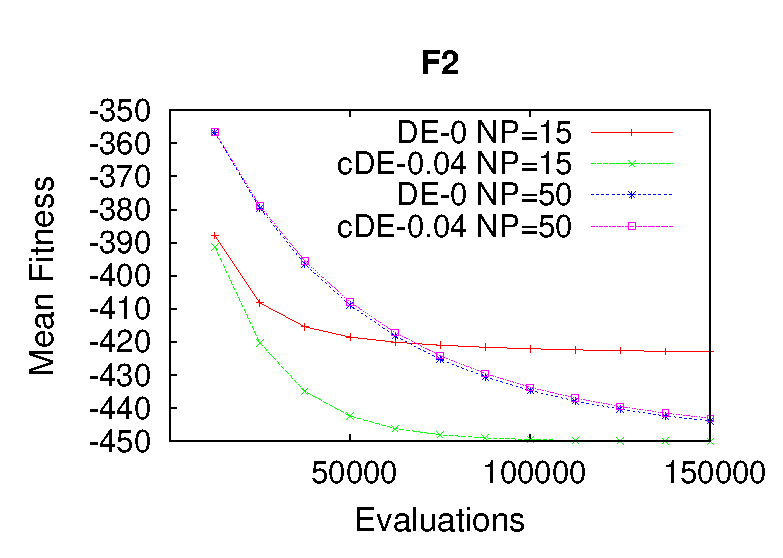
\includegraphics[width=0.27\textwidth]{images/Pop15_50/F2.eps} & 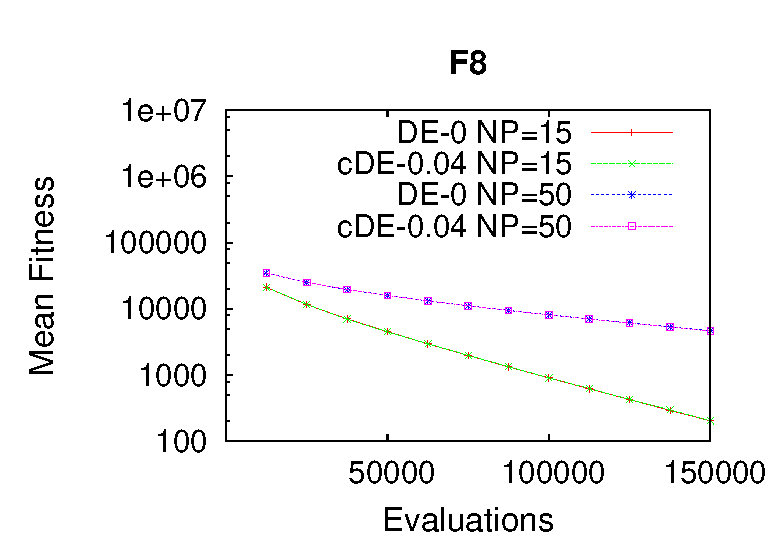
\includegraphics[width=0.27\textwidth]{images/Pop15_50/F8.eps}  \\
  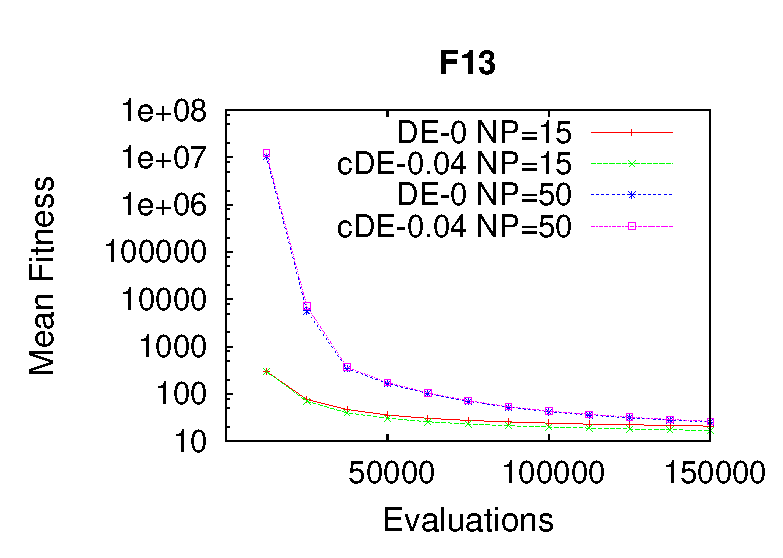
\includegraphics[width=0.27\textwidth]{images/Pop15_50/F13.eps} & 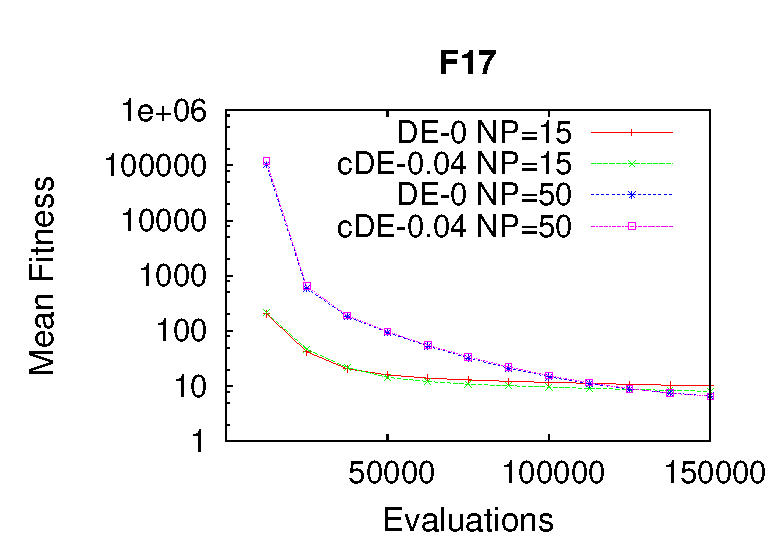
\includegraphics[width=0.27\textwidth]{images/Pop15_50/F17.eps}  \\
\end{tabular}
\caption{Evolution of the mean obtained by \DE{} and \CDE{}-0.04 with different population sizes}
\label{fig:pop}
\end{figure}

\begin{figure}[!t]
\centering
\includegraphics[width=0.33\textwidth]{images/Pop15_50/F17_boxplots.eps}
\caption{Boxplots of results obtained by \DE{} and \CDE{}-0.04 with different population sizes (F17)}
\label{fig:pop_f17_boxplots}
\end{figure}

%%\subsection{Third Set of Experiments: Crossover Rate}
%%
%%The increase in the $CR$ value implies that the number of times where only one variable is taken from the mutant vector decreases.
%%%
%%In fact, it was previously shown that, with the exp crossover, this happens with a probability equal to
%%$(1 - CR) \times 100$.
%%%
%%Thus, the increase in $CR$ implies that the new schemes proposed here are used a lower number of times.
%%%
%%For this reason, it is important to analyze the effects of large $CR$ values on the results obtained with \DE{} and \CDE{}.
%%%
%%In this study, the schemes \DE{} and \CDE{}-0.04 were analyzed for the following $CR$ values: 0.5, 0.6, 0.7, 0.8, and 0.9.
%%%
%%Four problems where \CDE{}-0.04 was shown to be beneficial in previous experiments were selected.
%%%
%%Specifically, they were F2, F3, F9 and F11.
%%
%%\figurename~\ref{fig:cr} shows the mean and median obtained by \DE{} and \CDE{}-0.04 with the different values of $CR$ in 150$\,$000 function evaluations.
%%%
%%The results of the statistical tests comparing \DE{} and \CDE{}-0.04 for each $CR$ value are shown in Table~\ref{tab:cr_stats}.
%%%
%%In the case of F2 and F3, \CDE{}-0.04 is better than \DE{} regardless of the $CR$ value considered, showing that the effects
%%of the modifications included in this paper can be significant even when considering large $CR$ values.
%%%
%%However, the statistical tests show that in F9 and F11, the differences are not significant when considering the largest $CR$ values.
%%%
%%This is not overly surprising because for values close to one, the probabilities of applying the new proposal are much lower.
%%%
%%Similar analyses were undertaken for the remaining problems where \CDE{}-0.04 had shown benefits in previous experiments.
%%%
%%This reveals that the only problems where the benefits disappear when $CR = 0.9$ are F9 and F11.
%%%
%%Thus, in general, the benefits can be obtained for a large range of $CR$ values.
%%
%%\begin{figure*}[!t]
%%\centering
%%\begin{tabular}{cc}
%%  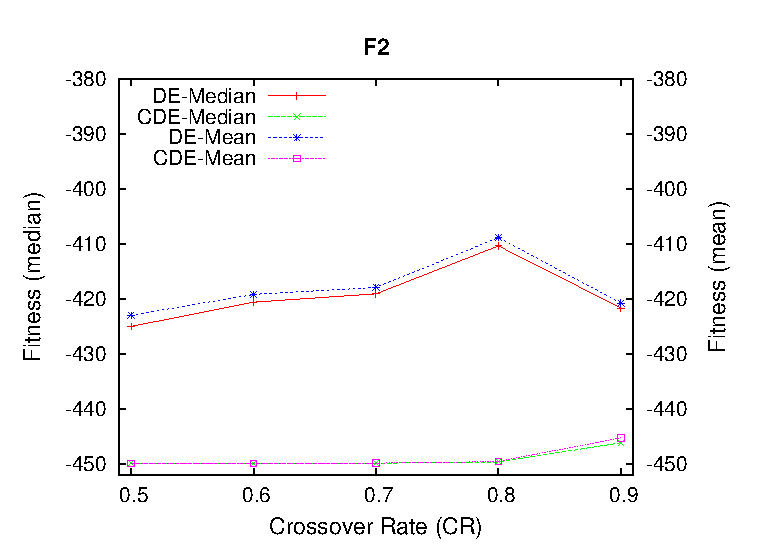
\includegraphics[width=0.40\textwidth]{images/CR_150000/F2_CR_P15_ReinitRandom_50} & 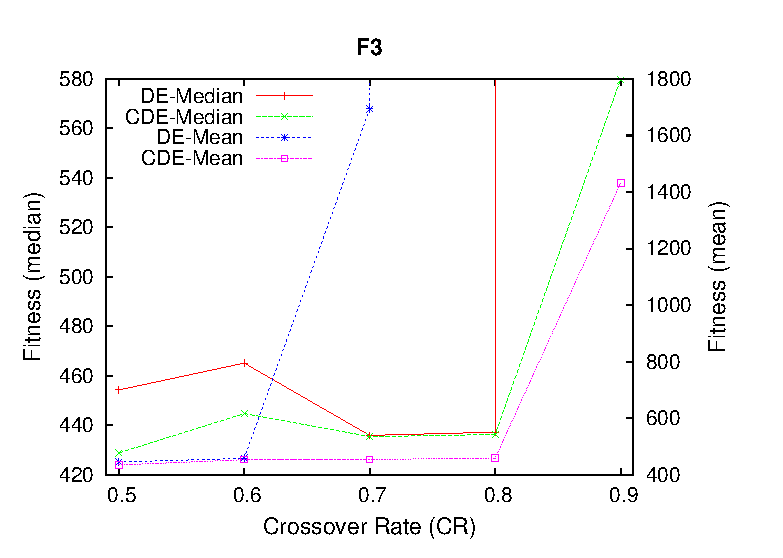
\includegraphics[width=0.40\textwidth]{images/CR_150000/F3_CR_P15_ReinitRandom_50}  \\
%%  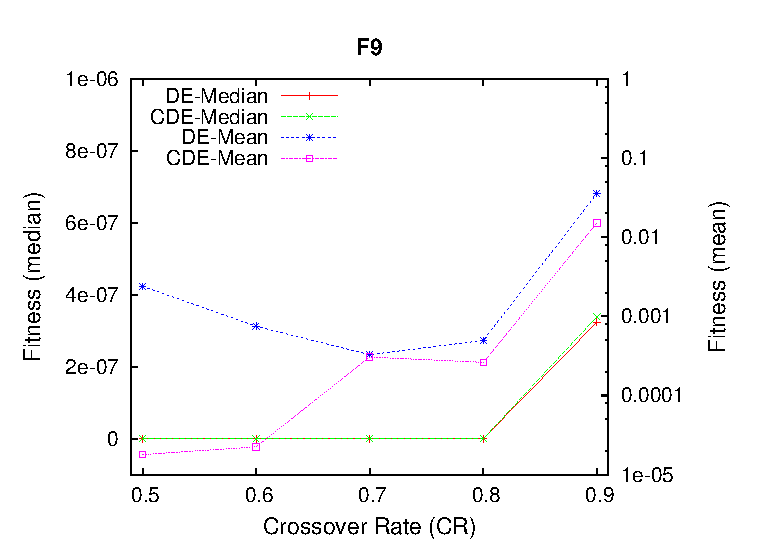
\includegraphics[width=0.40\textwidth]{images/CR_150000/F9_CR_P15_ReinitRandom_50} & 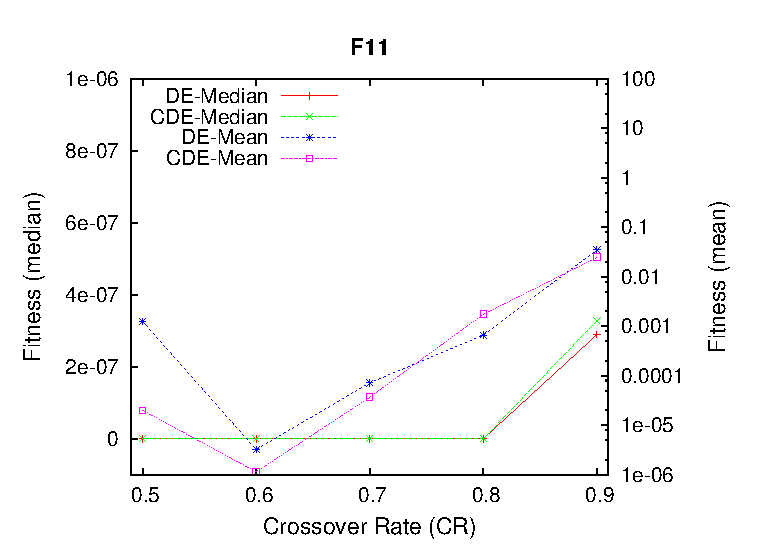
\includegraphics[width=0.40\textwidth]{images/CR_150000/F11_CR_P15_ReinitRandom_50}  \\
%%\end{tabular}
%%\caption{Mean and median obtained by \DE{} and \CDE{} with different values of \textsc{cr} in 150$\,$000 function evaluations}
%%\label{fig:cr}
%%\end{figure*}
%%
%%Note that in several problems, like F3, the $CR$ selected has a large impact on the quality of the results.
%%%
%%For this reason, a more robust scheme might be obtained by including an adaptive strategy for setting the $CR$ parameter.
%%%
%%In any case, this is a known fact~\cite{Montgomery:10}, and the most interesting conclusion of the comparison carried out herein is that
%%our schemes can provide benefits regardless of the $CR$ value adopted, and thus
%%we expect these benefits to be maintained when integrated with adaptive schemes.
%%
%%\begin{table}[!t]
%\renewcommand{\arraystretch}{1.4}
\caption{Statistical comparison of \textsc{de} vs. \textsc{cde}-0.04 with different values of \textsc{cr} in 150,000 function evaluations}
\label{tab:cr_stats}
\centering
\begin{scriptsize}
\begin{tabular}{c c c c c c}
\hline
               & \textsc{cr = 0.5} & \textsc{cr = 0.6} & \textsc{cr = 0.7} & \textsc{cr = 0.8} & \textsc{cr = 0.9} \\ \hline
F2             & $\uparrow$        & $\uparrow$        & $\uparrow$        & $\uparrow$        & $\uparrow$        \\ \hline
F3             & $\uparrow$        & $\uparrow$        & $\uparrow$        & $\uparrow$        & $\uparrow$        \\ \hline
F9             & $\uparrow$        & $\uparrow$        & $\uparrow$        & $\uparrow$        & $\leftrightarrow$ \\ \hline
F11            & $\uparrow$        & $\uparrow$        & $\leftrightarrow$ & $\leftrightarrow$ & $\leftrightarrow$ \\ \hline
\end{tabular}
\end{scriptsize}
\end{table}


\begin{table}[!t]
%\renewcommand{\arraystretch}{1.4}
\caption{Results obtained with \textsc{DE} by adapting \textsc{F} with different schemes (150.000 evaluations)}
\label{tab:adaptive_de}
\centering
\begin{scriptsize}
\begin{tabular}{c || c c c | c c c | c c c }
\hline
 & \multicolumn{3}{|c|}{SaDE} & \multicolumn{3}{|c}{j\textsc{de}} & \multicolumn{3}{|c}{\textsc{jade}} \\ \hline
    & Median                & Mean                  & Stat.             & Median                & Mean                 & Stat.             & Median                & Mean                  & Stat.             \\ \hline
F1  & $0$                   & $0$                   & $\leftrightarrow$ & $0$                   & $0$                  & $\leftrightarrow$ & $0$                   & $0$                   & $\leftrightarrow$ \\ \hline
F2  & $1.65$                & $3.88$                & $\uparrow$        & $14.49$               & $17.26$              & $\uparrow$        & $0.35$                & $0.35$                & $\uparrow$        \\ \hline
F3  & $28.92$               & $40.61$               & $\downarrow$      & $40.53$               & $45.69$              & $\leftrightarrow$ & $53.54$               & $58.73$               & $\uparrow$        \\ \hline
F4  & $0$                   & $0.28$                & $\uparrow$        & $0$                   & $0.45$               & $\uparrow$        & $0$                   & $9.94 \cdot 10^{-4}$  & $\downarrow$      \\ \hline
F5  & $0$                   & $4.45 \cdot 10^{-4}$  & $\uparrow$        & $0$                   & $2.60 \cdot 10^{-4}$ & $\uparrow$        & $0$                   & $2.95 \cdot 10^{-5}$  & $\leftrightarrow$ \\ \hline
F6  & $8.52 \cdot 10^{-14}$ & $8.52 \cdot 10^{-14}$ & $\leftrightarrow$ & $5.68 \cdot 10^{-14}$ & $4.95 \cdot 10^{-4}$ & $\uparrow$        & $8.52 \cdot 10^{-14}$ & $1.13 \cdot 10^{-13}$ & $\uparrow$        \\ \hline
F7  & $0$                   & $0$                   & $\leftrightarrow$ & $0$                   & $0$                  & $\leftrightarrow$ & $0$                   & $3.33 \cdot 10^{-19}$ & $\leftrightarrow$ \\ \hline
F8  & $206.31$              & $216.90$              & $\uparrow$        & $175.50$              & $184.54$             & $\downarrow$      & $526.91$              & $544.28$              & $\uparrow$        \\ \hline
F9  & $0$                   & $1.50 \cdot 10^{-2}$  & $\uparrow$        & $0$                   & $9.27 \cdot 10^{-3}$ & $\uparrow$        & $0$                   & $2.55 \cdot 10^{-4}$  & $\uparrow$        \\ \hline
F10 & $4.65 \cdot 10^{-20}$ & $3.82 \cdot 10^{-2}$  & $**$               & $4.96 \cdot 10^{-20}$ & $5.25 \cdot 10^{-2}$ & $**$               & $2.68 \cdot 10^{-19}$ & $1.04 \cdot 10^{-3}$  & $\uparrow$        \\ \hline
F11 & $0$                   & $1.61 \cdot 10^{-3}$  & $\uparrow$        & $0$                   & $5.03 \cdot 10^{-3}$ & $\uparrow$        & $0$                   & $3.35 \cdot 10^{-4}$  & $\uparrow$        \\ \hline
F12 & $4.17 \cdot 10^{-17}$ & $1.91 \cdot 10^{-4}$  & $\leftrightarrow$ & $4.15 \cdot 10^{-17}$ & $7.90 \cdot 10^{-3}$ & $\leftrightarrow$ & $1.62 \cdot 10^{-16}$ & $1.44 \cdot 10^{-4}$  & *                 \\ \hline
F13 & $4.05$                & $16.49$               & $\downarrow$      & $4.10$                & $18.29$              & $**$               & $20.77$               & $22.07$               & $\uparrow$        \\ \hline
F14 & $1.78 \cdot 10^{-15}$ & $0.25$                & $\uparrow$        & $2.44 \cdot 10^{-17}$ & $0.28$               & $\uparrow$        & $2.58 \cdot 10^{-17}$ & $0.19$                & $\uparrow$        \\ \hline
F15 & $4.89 \cdot 10^{-27}$ & $8.23 \cdot 10^{-3}$  & $\uparrow$        & $5.21 \cdot 10^{-27}$ & $4.61 \cdot 10^{-3}$ & $\uparrow$        & $8.64 \cdot 10^{-25}$ & $2.22 \cdot 10^{-19}$ & $\uparrow$        \\ \hline
F16 & $4.26 \cdot 10^{-17}$ & $9.29 \cdot 10^{-4}$  & $\leftrightarrow$ & $1.62 \cdot 10^{-18}$ & $7.71 \cdot 10^{-3}$ & $\leftrightarrow$ & $3.92 \cdot 10^{-16}$ & $2.37 \cdot 10^{-4}$  & *                 \\ \hline
F17 & $4.69$                & $11.57$               & $\uparrow$        & $6.58$                & $13.49$              & $\uparrow$        & $2.48$                & $5.95$                & $\leftrightarrow$ \\ \hline
F18 & $3.37 \cdot 10^{-17}$ & $4.28 \cdot 10^{-2}$  & $**$               & $3.23 \cdot 10^{-17}$ & $0.10$               & $*$               & $6.73 \cdot 10^{-14}$ & $6.21 \cdot 10^{-2}$  & *                 \\ \hline
F19 & $4.03 \cdot 10^{-23}$ & $2.92 \cdot 10^{-2}$  & $\uparrow$        & $2.62 \cdot 10^{-23}$ & $3.54 \cdot 10^{-2}$ & $\uparrow$        & $4.26 \cdot 10^{-21}$ & $3.71 \cdot 10^{-5}$  & $\uparrow$        \\ \hline
\end{tabular}
\end{scriptsize}
\end{table}


\subsection{Third Set of Experiments: Adapting $F$}

Since the schemes that consider a non-static $F$ value have the effect of increasing the number of potential trial vectors created
by the vector generation strategies, it is very interesting to compare the new proposal against some of the most popular schemes
that consider a variable $F$ value.
%
Three different adaptive models were considered.
%
The first one belongs to the group of randomized $F$ values.
%
Specifically, we considered the random distribution applied in SaDE~\cite{Qin:09}, i.e., a Gaussian distribution
with mean 0.5 and standard deviation 0.3.
%
The \DE{} parameters were fixed as in previous experiments, with \NP{} $= 15$.
%
In addition, two adaptive schemes that rely on the feedback obtained during the execution were considered.
%
They were the adaptive schemes incorporated in jDE~\cite{Brest:06} and JADE~\cite{Zhang:09}.
%
In both cases, they were parameterized using the values proposed by their authors.
%
Specifically, in jDE the value $\tau$ was set to 0.1, while $F_{min}$ and $F_{max}$ were set to 0.1 and 0.9, respectively.
%
In JADE the parameter $c$ was set to 0.1.
%


%\begin{table}[!t]
%\renewcommand{\arraystretch}{1.4}
\caption{Comparison of errors obtained by \textsc{DE} and \textsc{CDE}-0.04 in 500,000 evaluations ($D = 100$)}
\label{tab:scalability_100}
\centering
\begin{scriptsize}
\begin{tabular}{c || c c c | c c c c}
\hline
 & \multicolumn{3}{|c|}{\textsc{de}} & \multicolumn{4}{|c}{\textsc{cde-0.04}} \\ \hline
    & Median                 & Mean                  & Std. Dev.             & Median                         & Mean                           & Std. Dev.                      & Stat. \\ \hline
F1  & $0$                    & $2.42 \cdot 10^{-4}$  & $7.68 \cdot 10^{-3}$  & $0$                            & $0$                            & $0$                            & $\leftrightarrow$\\ \hline
F2  & $46.59$                & $47.27$               & $16.13$               & $\mathbf{4.43 \cdot 10^{-2}}$  & $\mathbf{4.62 \cdot 10^{-2}}$  & $\mathbf{1.15 \cdot 10^{-2}}$  & $\uparrow$ \\ \hline
F3  & $118.45$               & $118.93$              & $47.78$               & $\mathbf{103.13}$              & $\mathbf{103.91}$              & $\mathbf{41.95}$               & $\uparrow$ \\ \hline
F4  & $0$                    & $3.06 \cdot 10^{-2}$  & $0.32$                & $\mathbf{0}$                   & $\mathbf{2.32 \cdot 10^{-9}}$  & $\mathbf{7.35 \cdot 10^{-8}}$  & $\uparrow$ \\ \hline
F5  & $0$                    & $2.91 \cdot 10^{-4}$  & $4.70 \cdot 10^{-3}$  & $\mathbf{0}$                   & $\mathbf{2.00 \cdot 10^{-7}}$  & $\mathbf{6.32 \cdot 10^{-6}}$  & $\uparrow$ \\ \hline
F6  & $1.13 \cdot 10^{-13}$  & $1.90 \cdot 10^{-3}$  & $2.04 \cdot 10^{-2}$  & $\mathbf{1.13 \cdot 10^{-13}}$ & $\mathbf{1.42 \cdot 10^{-13}}$ & $\mathbf{2.03 \cdot 10^{-14}}$ & $\uparrow$ \\ \hline
F7  & $0$                    & $0$                   & $0$                   & $0$                            & $0$                            & $0$                            & $\leftrightarrow$\\ \hline
F8  & $357.94$               & $369.57$              & $94.27$               & $366.42$                       & $375.78$                       & $95.18$                        & $\leftrightarrow$\\ \hline
F9  & $0$                    & $4.14 \cdot 10^{-7}$  & $1.31 \cdot 10^{-5}$  & $0$                            & $0$                            & $0$                            & $\leftrightarrow$\\ \hline
F10 & $2.54 \cdot 10^{-20}$  & $2.89 \cdot 10^{-20}$ & $1.73 \cdot 10^{-20}$ & $\mathbf{2.01 \cdot 10^{-20}}$ & $\mathbf{2.25 \cdot 10^{-20}}$ & $\mathbf{1.28 \cdot 10^{-20}}$ & $\uparrow$ \\ \hline
F11 & $0$                    & $2.87 \cdot 10^{-4}$  & $8.45 \cdot 10^{-3}$  & $0$                            & $0$                            & $0$                            & $\leftrightarrow$\\ \hline
F12 & $2.78 \cdot 10^{-17}$  & $0.28$                & $9.10$                & $4.02 \cdot 10^{-17}$          & $2.10 \cdot 10^{-10}$          & $5.49 \cdot 10^{-9}$           & **          \\ \hline
F13 & $71.44$                & $70.24$               & $378.29$              & $\mathbf{53.28}$               & $\mathbf{49.95}$               & $\mathbf{35.52}$               & $\uparrow$ \\ \hline
F14 & $8.69 \cdot 10^{-18}$  & $4.55 \cdot 10^{-2}$  & $0.33$                & ${7.60 \cdot 10^{-18}}$        & ${4.98 \cdot 10^{-2}}$         & ${0.29}$                       & *          \\ \hline
F15 & $1.50 \cdot 10^{-29}$  & $6.15 \cdot 10^{-29}$ & $2.64 \cdot 10^{-28}$ & $\mathbf{0}$                   & $\mathbf{3.38 \cdot 10^{-31}}$ & $\mathbf{7.35 \cdot 10^{-31}}$ & $\uparrow$ \\ \hline
F16 & $2.99 \cdot 10^{-17}$  & $9.16 \cdot 10^{-16}$ & $2.66 \cdot 10^{-14}$ & ${3.14 \cdot 10^{-17}}$        & ${1.26 \cdot 10^{-16}}$        & ${9.54 \cdot 10^{-16}}$        & **          \\ \hline
F17 & $4.65$                 & $11.34$               & $15.32$               & $\mathbf{2.85}$                & $\mathbf{8.26}$                & $\mathbf{12.20}$               & $\uparrow$ \\ \hline
F18 & $3.98 \cdot 10^{-17}$  & $3.29 \cdot 10^{-2}$  & $0.21$                & $\mathbf{3.77 \cdot 10^{-17}}$ & $\mathbf{2.39 \cdot 10^{-2}}$  & $\mathbf{0.22}$                & $\uparrow$ \\ \hline
F19 & $2.60 \cdot 10^{-24}$  & $1.21 \cdot 10^{-23}$ & $5.74 \cdot 10^{-23}$ & $\mathbf{8.19 \cdot 10^{-27}}$ & $\mathbf{3.73 \cdot 10^{-26}}$ & $\mathbf{9.93 \cdot 10^{-26}}$ & $\uparrow$ \\ \hline
\end{tabular}
\end{scriptsize}
\end{table}


\begin{table}[!t]
%\renewcommand{\arraystretch}{1.4}
\caption{Comparison of errors obtained by \textsc{DE} and \textsc{CDE}-0.04 in 1,000,000 evaluations ($D = 200$)}
\label{tab:scalability_200}
\centering
\begin{scriptsize}
\begin{tabular}{c || c c c | c c c c}
\hline
 & \multicolumn{3}{|c|}{\textsc{de}} & \multicolumn{4}{|c}{\textsc{cde-0.04}} \\ \hline
    & Median                 & Mean                  & Std. Dev.             & Median                         & Mean                           & Std. Dev.                      & Stat.               \\ \hline
F1  & $0$                    & $0$                   & $1.79 \cdot 10^{-14}$ & $0$                            & $0$                            & $0$                            & $\leftrightarrow$   \\ \hline
F2  & $65.83$                & $65.89$               & $17.21$               & $\mathbf{1.43}$                & $\mathbf{1.46}$                & $\mathbf{0.19}$                & $\uparrow$          \\ \hline
F3  & $243.92$               & $243.43$              & $59.87$               & $\mathbf{230.86}$              & $\mathbf{227.26}$              & $\mathbf{53.34}$               & $\uparrow$          \\ \hline
F4  & $0$                    & $8.13 \cdot 10^{-2}$  & $0.71$                & ${0}$                          & ${4.34 \cdot 10^{-2}}$         & ${0.51}$                       & $\leftrightarrow$   \\ \hline
F5  & $0$                    & $3.23 \cdot 10^{-4}$  & $5.38 \cdot 10^{-3}$  & ${0}$                          & ${8.74 \cdot 10^{-5}}$         & ${2.04 \cdot 10^{-3}}$         & $\leftrightarrow$   \\ \hline
F6  & $1.98 \cdot 10^{-13}$  & $5.62 \cdot 10^{-3}$  & $4.14 \cdot 10^{-2}$  & $\mathbf{1.98 \cdot 10^{-13}}$ & $\mathbf{1.98 \cdot 10^{-13}}$ & $\mathbf{2.18 \cdot 10^{-14}}$          & $\uparrow$   \\ \hline
F7  & $0$                    & $0$                   & $0$                   & $0$                            & $0$                            & $0$                            & $\leftrightarrow$   \\ \hline
F8  & $4381.43$              & $4412.40$             & $609.19$              & $4404.58$                      & $4423.31$                      & $617.84$                       & $\leftrightarrow$   \\ \hline
F9  & $0$                    & $0$                   & $0$                   & $0$                            & $1.69 \cdot 10^{-10}$          & $5.36 \cdot 10^{-9}$           & $\leftrightarrow$   \\ \hline
F10 & $2.69 \cdot 10^{-20}$  & $3.12 \cdot 10^{-20}$ & $4.51 \cdot 10^{-20}$ & $\mathbf{2.05 \cdot 10^{-20}}$ & $\mathbf{2.14 \cdot 10^{-20}}$ & $\mathbf{1.03 \cdot 10^{-20}}$ & $\uparrow$          \\ \hline
F11 & $0$                    & $0$                   & $0$                   & $0$                            & $2.31 \cdot 10^{-10}$          & $7.32 \cdot 10^{-9}$           & $\leftrightarrow$   \\ \hline
F12 & $8.33 \cdot 10^{-17}$  & $1.81 \cdot 10^{-2}$  & $0.56$                & $\mathbf{8.32 \cdot 10^{-17}}$ & $\mathbf{5.45 \cdot 10^{-5}}$  & $\mathbf{1.07 \cdot 10^{-3}}$  & $\uparrow$          \\ \hline
F13 & $147.99$               & $149.34$              & $63.67$               & $\mathbf{129.86}$              & $\mathbf{129.89}$              & $\mathbf{48.01}$               & $\uparrow$          \\ \hline
F14 & $1.03 \cdot 10^{-17}$  & $9.00 \cdot 10^{-2}$  & $0.56$                & ${9.17 \cdot 10^{-18}}$        & $0.11$                         & ${0.59}$                       & *                   \\ \hline
F15 & $9.94 \cdot 10^{-30}$  & $1.92 \cdot 10^{-7}$  & $6.09 \cdot 10^{-6}$  & $\mathbf{0}$                   & $\mathbf{1.48 \cdot 10^{-31}}$ & $\mathbf{4.51 \cdot 10^{-31}}$ & $\uparrow$          \\ \hline
F16 & $5.56 \cdot 10^{-17}$  & $3.52 \cdot 10^{-4}$  & $8.23 \cdot 10^{-3}$  & ${5.62 \cdot 10^{-17}}$        & ${2.40 \cdot 10^{-5}}$         & ${4.76 \cdot 10^{-4}}$         & $\leftrightarrow$   \\ \hline
F17 & $6.07$                 & $16.29$               & $23.80$               & $\mathbf{3.80}$                & $\mathbf{10.33}$               & $\mathbf{17.85}$               & $\uparrow$          \\ \hline
F18 & $6.46 \cdot 10^{-17}$  & $5.96 \cdot 10^{-2}$  & $0.28$                & $\mathbf{5.88 \cdot 10^{-17}}$ & $\mathbf{5.89 \cdot 10^{-2}}$  & $\mathbf{0.30}$                & $\uparrow$   \\ \hline
F19 & $1.31 \cdot 10^{-24}$  & $3.81 \cdot 10^{-3}$  & $0.12$                & $\mathbf{3.47 \cdot 10^{-27}}$ & $\mathbf{1.23 \cdot 10^{-26}}$ & $\mathbf{4.37 \cdot 10^{-26}}$ & $\uparrow$          \\ \hline
\end{tabular}
\end{scriptsize}
\end{table}


\begin{table}[!t]
%\renewcommand{\arraystretch}{1.4}
\caption{Comparison of errors obtained by \textsc{DE} and \textsc{CDE}-0.04 in 2,500,000 evaluations ($D = 500$)}
\label{tab:scalability_500}
\centering
\begin{scriptsize}
\begin{tabular}{c || c c c | c c c c}
\hline
 & \multicolumn{3}{|c|}{\textsc{de}} & \multicolumn{4}{|c}{\textsc{cde-0.04}} \\ \hline
    & Median                 & Mean                  & Std. Dev.             & Median                         & Mean                           & Std. Dev.                      & Stat.               \\ \hline
F1  & $0$                    & $0.43$                & $13.71$               & $\mathbf{0}$                   & $\mathbf{0}$                   & $\mathbf{0}$                   & $\uparrow$          \\ \hline
F2  & $90.72$                & $89.82$               & $16.67$               & $\mathbf{17.07}$               & $\mathbf{17.10}$               & $\mathbf{0.75}$                & $\uparrow$          \\ \hline
F3  & $658.36$               & $59373.95$            & $1330246$             & $\mathbf{637.85}$              & $\mathbf{635.42}$              & $\mathbf{78.47}$               & $\uparrow$          \\ \hline
F4  & $0$                    & $0.75$                & $2.92$                & $\mathbf{0}$                   & $\mathbf{0.22}$                & $\mathbf{1.42}$                & $\uparrow$          \\ \hline
F5  & $0$                    & $1.34 \cdot 10^{-2}$  & $0.25$                & $\mathbf{0}$                   & $\mathbf{1.23 \cdot 10^{-5}}$  & $\mathbf{3.89 \cdot 10^{-4}}$  & $\uparrow$          \\ \hline
F6  & $4.54 \cdot 10^{-13}$  & $6.61 \cdot 10^{-3}$  & $2.71 \cdot 10^{-2}$  & $\mathbf{4.54 \cdot 10^{-13}}$ & $\mathbf{4.54 \cdot 10^{-13}}$ & $\mathbf{2.42 \cdot 10^{-14}}$ & $\uparrow$          \\ \hline
F7  & $0$                    & $7.56 \cdot 10^{-9}$  & $2.39 \cdot 10^{-7}$  & $0$                            & $0$                            & $0$                            & $\leftrightarrow$   \\ \hline
F8  & $53737.73$             & $53724.33$            & $3928.97$             & $53335.88$                     & $53434.75$                     & $3939.66$                      & $\leftrightarrow$   \\ \hline
F9  & $0$                    & $2.39 \cdot 10^{-4}$  & $6.25 \cdot 10^{-3}$  & $0$                            & $2.21 \cdot 10^{-5}$           & $4.94 \cdot 10^{-4}$           & $\leftrightarrow$   \\ \hline
F10 & $2.96 \cdot 10^{-20}$  & $1.10 \cdot 10^{-2}$  & $0.34$                & $\mathbf{2.42 \cdot 10^{-20}}$ & $\mathbf{1.04 \cdot 10^{-3}}$  & $\mathbf{3.31 \cdot 10^{-2}}$  & $\uparrow$          \\ \hline
F11 & $0$                    & $5.82 \cdot 10^{-5}$  & $9.42 \cdot 10^{-4}$  & $0$                            & $2.70 \cdot 10^{-4}$           & $8.09 \cdot 10^{-3}$           & $\leftrightarrow$   \\ \hline
F12 & $1.66 \cdot 10^{-16}$  & $0.15$                & $3.59$                & $\mathbf{1.38 \cdot 10^{-16}}$ & $\mathbf{3.90 \cdot 10^{-4}}$  & $\mathbf{2.17 \cdot 10^{-3}}$  & $\uparrow$          \\ \hline
F13 & $429.37$               & $440.70$              & $274.80$              & $\mathbf{405.87}$              & $\mathbf{404.27}$              & $\mathbf{82.05}$               & $\uparrow$          \\ \hline
F14 & $1.80 \cdot 10^{-17}$  & $0.39$                & $1.63$                & $\mathbf{1.64 \cdot 10^{-17}}$ & $\mathbf{0.30}$                & $\mathbf{1.17}$                & $\uparrow$          \\ \hline
F15 & $1.95 \cdot 10^{-29}$  & $3.20 \cdot 10^{-3}$  & $0.10$                & $\mathbf{0}$                   & $\mathbf{1.34 \cdot 10^{-31}}$ & $\mathbf{4.24 \cdot 10^{-31}}$ & $\uparrow$          \\ \hline
F16 & $1.11 \cdot 10^{-16}$  & $8.57 \cdot 10^{-3}$  & $0.23$                & $\mathbf{1.11 \cdot 10^{-16}}$ & $\mathbf{4.08 \cdot 10^{-4}}$  & $\mathbf{1.98 \cdot 10^{-3}}$  & $\uparrow$          \\ \hline
F17 & $73.64$                & $294.66$              & $5220.16$             & $\mathbf{70.60}$               & $\mathbf{54.09}$               & $\mathbf{44.35}$               & $\uparrow$          \\ \hline
F18 & $3.37 \cdot 10^{-16}$  & $0.15$                & $0.64$                & $1.88 \cdot 10^{-16}$          & $0.18$                         & $0.74$                         & $\leftrightarrow$   \\ \hline
F19 & $1.24 \cdot 10^{-24}$  & $1.05 \cdot 10^{-3}$  & $3.31 \cdot 10^{-2}$  & $\mathbf{3.41 \cdot 10^{-27}}$ & $\mathbf{2.54 \cdot 10^{-22}}$ & $\mathbf{8.03 \cdot 10^{-21}}$ & $\uparrow$          \\ \hline
\end{tabular}
\end{scriptsize}
\end{table}




\begin{table}[!t]
%\renewcommand{\arraystretch}{1.4}
\caption{Comparison of errors obtained by \textsc{DE} and \textsc{CDE}-0.04 in 3,000,000 evaluations with the CEC'10 Benchmark Test Suite}
\label{tab:scalability_1000_cec}
\centering
\begin{scriptsize}
\begin{tabular}{c || c c c | c c c c}
\hline
 & \multicolumn{3}{|c|}{\textsc{de}} & \multicolumn{4}{|c}{\textsc{cde}} \\ \hline
    & Median                 & Mean                  & Std. Dev.             & Median                         & Mean                           & Std. Dev.                      & Stat.               \\ \hline
F1  & $4.17 \cdot 10^{-17}$ & $2.56  \cdot 10^{5}$  & $5.39 \cdot 10^{6}$  & $\mathbf{6.84 \cdot 10^{-21}}$ & $\mathbf{1.33 \cdot 10^{1}}$  & $\mathbf{2.55 \cdot 10^{2}}$ & $\uparrow$ \\ \hline
F2  & $1.11 \cdot 10^{2}$   & $1.11  \cdot 10^{2}$  & $2.90 \cdot 10^{1}$  & $\mathbf{3.48 \cdot 10^{1}}$   & $\mathbf{3.53 \cdot 10^{1}}$  & $\mathbf{8.40}$ & $\uparrow$ \\ \hline
F3  & $1.74 \cdot 10^{-13}$ & $3.67  \cdot 10^{-2}$ & $2.10 \cdot 10^{-1}$ & $\mathbf{1.03 \cdot 10^{-13}}$ & $\mathbf{1.17 \cdot 10^{-4}}$ & $\mathbf{7.7 \cdot 10^{-4}}$ & $\uparrow$ \\ \hline
F4  & $4.29 \cdot 10^{13}$  & $4.30  \cdot 10^{13}$ & $8.44 \cdot 10^{12}$ & $4.21 \cdot 10^{13}$  & $4.25 \cdot 10^{13}$ & $8.63 \cdot 10^{12}$ & $\leftrightarrow$ \\ \hline
F5  & $1.70 \cdot 10^{8}$   & $1.70  \cdot 10^{8}$  & $2.43 \cdot 10^{7}$  & $1.69 \cdot 10^{8}$   & $1.69 \cdot 10^{8}$  & $2.45 \cdot 10^{7}$ & $\leftrightarrow$ \\ \hline
F6  & $1.35 \cdot 10^{3}$   & $9.84  \cdot 10^{4}$  & $3.46 \cdot 10^{5}$  & $\mathbf{9.52 \cdot 10^{2}}$   & $\mathbf{8.58 \cdot 10^{4}}$  & $\mathbf{3.38 \cdot 10^{5}}$ & $\uparrow$ \\ \hline
F7  & $1.46 \cdot 10^{7}$   & $1.80  \cdot 10^{7}$  & $3.14 \cdot 10^{7}$  & $\mathbf{1.42 \cdot 10^{7}}$   & $\mathbf{1.71 \cdot 10^{7}}$  & $\mathbf{1.22 \cdot 10^{7}}$ & $\uparrow$ \\ \hline
F8  & $4.85 \cdot 10^{7}$   & $1.33  \cdot 10^{11}$ & $1.92 \cdot 10^{12}$ & $\mathbf{4.68 \cdot 10^{7}}$   & $\mathbf{6.69 \cdot 10^{7}}$  & $\mathbf{3.63 \cdot 10^{7}}$ & $\uparrow$ \\ \hline
F9  & $8.41 \cdot 10^{8}$   & $8.39  \cdot 10^{8}$  & $5.61 \cdot 10^{7}$  & $\mathbf{8.35 \cdot 10^{8}}$   & $\mathbf{8.35 \cdot 10^{8}}$  & $\mathbf{5.67 \cdot 10^{7}}$ & $\uparrow$ \\ \hline
F10 & $5.02 \cdot 10^{3}$   & $5.01  \cdot 10^{3}$  & $2.15 \cdot 10^{2}$  & $\mathbf{4.99 \cdot 10^{3}}$   & $\mathbf{5.00 \cdot 10^{3}}$  & $\mathbf{2.13 \cdot 10^{2}}$ & $\uparrow$ \\ \hline
F11 & $2.062 \cdot 10^{2}$  & $2.05  \cdot 10^{2}$  & $3.29$               & $\mathbf{2.061 \cdot 10^{2}}$  & $\mathbf{2.04 \cdot 10^{2}}$  & $\mathbf{3.65}$ & $\uparrow$ \\ \hline
F12 & $7.62 \cdot 10^{5}$   & $7.60  \cdot 10^{5}$  & $3.28 \cdot 10^{4}$  & $\mathbf{7.55 \cdot 10^{5}}$   & $\mathbf{7.54 \cdot 10^{5}}$  & $\mathbf{3.09 \cdot 10^{4}}$ & $\uparrow$ \\ \hline
F13 & $1.64 \cdot 10^{3}$   & $1.45  \cdot 10^{7}$  & $1.76 \cdot 10^{8}$  & $\mathbf{1.15 \cdot 10^{3}}$   & $\mathbf{1.62 \cdot 10^{3}}$  & $\mathbf{1.59 \cdot 10^{3}}$ & $\uparrow$ \\ \hline
F14 & $1.28 \cdot 10^{9}$   & $1.28  \cdot 10^{9}$  & $5.88 \cdot 10^{7}$  & $\mathbf{1.27 \cdot 10^{9}}$   & $\mathbf{1.26 \cdot 10^{9}}$  & $\mathbf{5.90 \cdot 10^{7}}$ & $\uparrow$ \\ \hline
F15 & $1.20 \cdot 10^{4}$   & $1.20  \cdot 10^{4}$  & $3.82 \cdot 10^{2}$  & $1.20 \cdot 10^{4}$   & $1.20 \cdot 10^{4}$  & $3.73 \cdot 10^{2}$ & $\leftrightarrow$ \\ \hline
F16 & $4.142 \cdot 10^{2}$  & $4.127 \cdot 10^{2}$  & $3.58$               & $\mathbf{4.141 \cdot 10^{2}}$  & $\mathbf{4.124 \cdot 10^{2}}$ & $\mathbf{3.85}$ & $\uparrow$ \\ \hline
F17 & $1.72 \cdot 10^{6}$   & $1.72  \cdot 10^{6}$  & $5.23 \cdot 10^{4}$  & $\mathbf{1.70 \cdot 10^{6}}$   & $\mathbf{1.69 \cdot 10^{6}}$  & $\mathbf{5.06 \cdot 10^{4}}$ & $\uparrow$ \\ \hline
F18 & $6.55 \cdot 10^{3}$   & $3.09  \cdot 10^{7}$  & $1.53 \cdot 10^{8}$  & $\mathbf{3.25 \cdot 10^{3}}$   & $\mathbf{4.53 \cdot 10^{3}}$  & $\mathbf{3.26 \cdot 10^{3}}$ & $\uparrow$ \\ \hline
F19 & $4.64 \cdot 10^{6}$   & $4.63  \cdot 10^{6}$  & $2.63 \cdot 10^{5}$  & $\mathbf{4.62 \cdot 10^{6}}$   & $\mathbf{4.61 \cdot 10^{6}}$  & $\mathbf{2.73 \cdot 10^{5}}$ & $\uparrow$ \\ \hline
F20 & $2.07 \cdot 10^{3}$   & $4.10  \cdot 10^{7}$  & $2.54 \cdot 10^{8}$  & $\mathbf{1.71 \cdot 10^{3}}$   & $\mathbf{1.73 \cdot 10^{3}}$  & $\mathbf{3.76 \cdot 10^{2}}$ & $\uparrow$ \\ \hline
\end{tabular}
\end{scriptsize}
\end{table}





Table~\ref{tab:adaptive_de} shows the mean and median obtained by each of the models for the different benchmark functions.
%
In addition, the results of the statistical tests when comparing each model with \CDE{}-0.04 are shown.
%
The comparisons reveal that \CDE{}-0.04 is statistically better than the schemes that employ the adaptation of SaDE and jDE in 10 problems,
and worse in one problem.
%
They also show that \CDE{}-0.04 is statistically better than \DE{} with the JADE adaptation scheme in 11 problems and worse
in only one problem.
%
The above results show that the way of increasing diversity proposed here is preferable to the methods that adapt the $F$ value during the run.
%
Moreover, it also calls into question the robustness of those adaptive schemes that consider feedback to set the value of $F$.
%
%In our opinion, more research is required in this area.
%
%However, such an analysis is beyond the scope of this paper.

\subsection{Fourth Set of Experiments: Scalability}

It is also very interesting to check the relationship between the behavior of the new proposal and the dimensionality of the
problem.
%
It was shown that as the number of dimensions grows, the number of potential trials also grows.
%
However, while the growth in the search space is exponential, the growth in the potential trials is only polynomial
when exp crossover is considered.
%
Thus, it is not easy to predict the overall effect.

Regarding the parameterization of \DE{}, note that according to~\cite{Zhao:13}, the optimal $CR$ value usually depends on the dimensionality.
%
In order to avoid having to tune $CR$ for each dimension, the techniques proposed in that paper might be used.
%
However, for the set of problems considered, a fixed $CR$ value equal to $0.5$ allows obtaining competitive results
for the dimensions considered in this paper~\cite{LaTorre:11}.
%
Thus, in order to keep our approach as simple as possible,
\DE{} and \CDE{}-0.04 were executed with
the same parameterization as in the first set of experiments,
but considering several dimensionalities.
%
Specifically, the following values of $D$ were considered: 200, 500 and 1000.
%
The stopping criterion was set at $5000D$ in every case.
%
Tables~\ref{tab:scalability_200}, \ref{tab:scalability_500},
and \ref{tab:scalability_1000} show the mean, median and standard deviation
of both models for each of the dimensionalities tested.
%
The results of the statistical tests are also shown.
%
These show that both the median and mean errors increase as higher dimensionalities are used.
%
This was expected because while the search space size grows exponentially, the number of function evaluations increases only linearly.
%
In any event, the advantages of \CDE{}-0.04 remain clear and are even greater than for lower dimensionalities.
%
For instance, while for $D = 200$, \CDE{}-0.04 is statistically better than \DE{} in
10 problems, for $D = 1000$ the number of problems where \CDE{}-0.04 is better increases to 14.
%
It is also interesting to note that for the total number of statistical tests conducted in
the scalability analysis, \CDE{}-0.04 was superior to \DE{} in 38 out of the 57 cases, being inferior in only one case.
%
This indicates a clear superiority of the \CDE{}-0.04 scheme.

It is also remarkable that when dealing with the largest search spaces,
there are several cases where \DE{} yields very high mean values, while the behavior of
\CDE{}-0.04 does not degrade too much.
%
The reason is that the worst-case behavior of \DE{} is much worse than the worst-case behavior of \CDE{}-0.04.
%
Some of the problems where this happens are F3, F15 and F17 with $D = 500$, and F6, F13 and F15 with $D = 1000$.

\subsection{Fifth Set of Experiments: Other \DE{} variants}

\textcolor{red}{
The previous experiments have shown the advantages of incorporating our proposals in a basic
variant of \DE{}.
%
Since there are several non-hybrid \DE{} variants that have been successfully used to improve on the results obtained with \DE{} in the \textsc{soco} tests,
analyzing the combination of such \DE{} variants with the new proposals defined in this paper is quite interesting.
%
\textsc{gade}~\cite{Yang:11}, \textsc{gode}~\cite{Wang:11b} and j\textsc{de}lscop~\cite{Brest:11} are three non-hybrid \DE{} variants that have obtained promising results 
following quite different principles.
%
For this reason, they were selected for this study.
%
In every case the integration was done in a similar way.
%
Specifically, when the value $L$ generated by the crossover is equal to one, instead of using the original way of creating the trial vector,
our proposal is applied.
%
As in previous experiments, the parameter \HMR{} was set to 0.04 and $UpdateDenom$ to 10.
%
The remaining details and parameterization of the schemes were as proposed by their authors.
}

\textcolor{red}{
The \textsc{gade} scheme~\cite{Yang:11} is based on adapting the mutation strategy, as well as the $F$ and $CR$ parameters.
%
Among the mutation strategies, the greedy DE/current-to-pbest/2 is used, meaning that more intensification is induced.
%
As a result, larger population sizes might be preferred. 
%
In fact, in~\cite{Yang:11}, the population size was set to 60.
%
Since the incorporation of our schemes move this balance towards exploration, \textsc{gade} and the new proposal (c\textsc{gade-0.04})
were tested with two different population sizes (\NP{} $= 15$ and \NP{} $= 60$).
%
Table~\ref{tab:gade} shows the mean and median obtained for each problem.
%
In addition, statistical tests were used to compare \textsc{gade} and c\textsc{gade-0.04} for each $NP$ value.
%
As in previous cases, the symbol $\uparrow$ is used to denote the superiority of the scheme that incorporates our proposals, i.e. c\textsc{gade-0.04}.
%
We can appreciate that when $NP$ is set to 15, the superiority of c\textsc{gade-0.04} is clear.
%
Since using a so low population size induces a larger degree of exploitation, increasing the diversity of trial vectors with the new proposals provides significant benefits.
%
Moreover, even when $NP$ is set to 60, the proposed schemes provides significant improvements in several cases.
%
However, for some problems using $NP = 60$ and increasing the diversity produce too much exploration, meaning that degradation appears.
%
This happens in problems where very low errors are obtained.
%
In such cases, in order to refine the solutions, small perturbations are required, so the schemes proposed in this paper delay the convergence.
%
Since there are some problems where c\textsc{gade-0.04} with $NP = 15$ performs better and there are other problems where \textsc{gade} with $NP = 60$ is preferred,
increasing the population size and our proposals should be regarded as alternative choices to balance exploration and exploitation that can be used together.
%
In general, in the case of c\textsc{gade-0.04} more diversity is induced, so a shorter population can be used, whereas in the case of \textsc{gade}, more intensification is promoted, so
larger populations are admissible.
}

\begin{table*}[!t]
%\renewcommand{\arraystretch}{1.4}
\caption{Comparison of errors obtained by \textsc{gade} and c\textsc{gade}-0.04 in 5,000,000 evaluations ($D = 1000$)}
\label{tab:gade}
\centering
\begin{scriptsize}
\begin{tabular}{c || c c | c c c || c c | c c c}
\hline
 & \multicolumn{5}{|c||}{\NP{} = 15} & \multicolumn{5}{|c}{\NP{} = 60} \\ \hline
 & \multicolumn{2}{|c|}{\textsc{gade}}      & \multicolumn{3}{|c||}{c\textsc{gade-0.04}}         & \multicolumn{2}{|c|}{\textsc{gade}} & \multicolumn{3}{|c}{c\textsc{gade-0.04}} \\ \hline
    & Median               & Mean                  & Median                        & Mean                          & St.               & Median               & Mean                          & Median                        & Mean                          & St.                \\ \hline
F1  & $0$                  & $0$                   & $0$                           & $0$                           & $\leftrightarrow$ & $0$                  & $0$                           & $0$                           & $0$                           & $\leftrightarrow$  \\ \hline
F2  & $39.6$               & $43.8$                & $\mathbf{10.6}$               & $\mathbf{11.6}$               & $\uparrow$        & $88.5$               & $86.3$                        & $\mathbf{33.4}$               & $\mathbf{34.9}$               & $\uparrow$         \\ \hline
F3  & $800.0$              & $791.9$               & $\mathbf{773.2}$              & $\mathbf{769.0}$              & $\uparrow$        & $945.5$              & $946.4$                       & $941.0$              & $966.5$              & $\leftrightarrow$  \\ \hline
F4  & $1.9$                & $2.8$                 & $1.9$                         & $2.4$                         & $\leftrightarrow$ & $0$                  & $0$                           & $0$                           & $0$                           & $\leftrightarrow$  \\ \hline
F5  & $0$                  & $2.7 \cdot 10^{-2}$   & $0$                           & $2.9 \cdot 10^{-2}$           & $\leftrightarrow$ & $0$                  & $1.3 \cdot 10^{-4}$           & $0$                           & $2.7 \cdot 10^{-4}$           & $\leftrightarrow$  \\ \hline
F6  & $1.3 \cdot 10^{-13}$ & $2.3 \cdot 10^{-13}$  & $1.3 \cdot 10^{-13}$          & $1.7 \cdot 10^{-13}$          & $\leftrightarrow$ & $1.8 \cdot 10^{-14}$ & $1.4 \cdot 10^{-11}$          & $\mathbf{1.8 \cdot 10^{-14}}$ & $\mathbf{2.3 \cdot 10^{-14}}$ & $\uparrow$         \\ \hline
F7  & $0$                  & $7.9 \cdot 10^{-17}$  & $0$                           & $0$                           & $\leftrightarrow$ & $0$                  & $0$                           & $0$                           & $0$                           & $\leftrightarrow$  \\ \hline
F8  & $17421.3$            & $17651.7$             & $\mathbf{11374.6}$            & $\mathbf{11498.0}$            & $\uparrow$        & $17242.3$            & $17670.5$                     & $\mathbf{15254.1}$            & $\mathbf{15316.7}$            & $\uparrow$         \\ \hline
F9  & $8.3 \cdot 10^{-2}$  & $1.0 \cdot 10^{-1}$   & $\mathbf{3.0 \cdot 10^{-2}}$  & $\mathbf{3.7 \cdot 10^{-2}}$  & $\uparrow$        & $\mathbf{0}$         & $\mathbf{7.5 \cdot 10^{-5}}$  & $0$                           & $1.1 \cdot 10^{-4}$           & $\downarrow$       \\ \hline
F10 & $20.9$               & $21.3$                & $\mathbf{1.0}$                & $\mathbf{7.9 \cdot 10^{-1}}$  & $\uparrow$        & $0$                  & $3.9 \cdot 10^{-1}$           & $\mathbf{0}$                  & $\mathbf{4.3 \cdot 10^{-2}}$  & $\uparrow$         \\ \hline
F11 & $8.3 \cdot 10^{-2}$  & $9.5 \cdot 10^{-2}$   & $\mathbf{3.0 \cdot 10^{-2}}$  & $\mathbf{3.7 \cdot 10^{-2}}$  & $\uparrow$        & $\mathbf{0}$         & $\mathbf{6.4 \cdot 10^{-5}}$  & $0$                           & $2.5 \cdot 10^{-4}$           & $\downarrow$       \\ \hline
F12 & $10.5$               & $14.8$                & $\mathbf{0}$                  & $\mathbf{3.5 \cdot 10^{-2}}$  & $\uparrow$        & $3.7 \cdot 10^{-12}$ & $3.4 \cdot 10^{-2}$           & $1.3 \cdot 10^{-11}$          & $1.5 \cdot 10^{-11}$          & **                 \\ \hline
F13 & $717.2$              & $712.5$               & $\mathbf{638.2}$              & $\mathbf{629.2}$              & $\uparrow$        & $715.1$              & $723.6$                       & $714.7$                       & $722.5$                       & $\leftrightarrow$  \\ \hline
F14 & $1.9$                & $2.2$                 & $\mathbf{9.9 \cdot 10^{-1}}$  & $\mathbf{1.42}$               & $\uparrow$        & $8.4 \cdot 10^{-11}$ & $19.33$                       & $1.6 \cdot 10^{-10}$          & $1.8 \cdot 10^{-10}$          & **                 \\ \hline
F15 & $\mathbf{3.1}$       & $\mathbf{3.0}$        & $3.1$                         & $4.0$                         & $\downarrow$      & $\mathbf{0}$         & $\mathbf{1.3 \cdot 10^{-2}}$  & $0$                           & $3.6 \cdot 10^{-2}$           & $\downarrow$       \\ \hline
F16 & $14.4$               & $18.2$                & $\mathbf{2.1 \cdot 10^{-2}}$  & $\mathbf{4.1 \cdot 10^{-2}}$  & $\uparrow$        & $2.4 \cdot 10^{-12}$ & $1.1 \cdot 10^{-5}$           & $5.1 \cdot 10^{-12}$          & $5.2 \cdot 10^{-12}$          & **                 \\ \hline
F17 & $239.5$              & $244.7$               & $\mathbf{227.0}$              & $\mathbf{222.6}$              & $\uparrow$        & $218.1$              & $220.9$                       & $219$                         & $220.5$                       & **                 \\ \hline
F18 & $1.0$                & $9.07 \cdot 10^{-1}$  & $\mathbf{4.2 \cdot 10^{-2}}$  & $\mathbf{3.3 \cdot 10^{-1}}$  & $\uparrow$        & $1.1 \cdot 10^{-7}$  & $2.2 \cdot 10^{-1}$           & $3.1 \cdot 10^{-7}$           & $6.4 \cdot 10^{-5}$           & **                 \\ \hline
F19 & $7.3$                & $7.8$                 & $\mathbf{0}$                  & $\mathbf{7.8 \cdot 10^{-1}}$  & $\uparrow$        & $0$                  & $2.8 \cdot 10^{-1}$           & $\mathbf{0}$                  & $\mathbf{8.7 \cdot 10^{-2}}$  & $\uparrow$         \\ \hline
\end{tabular}
\end{scriptsize}
\end{table*}


\textcolor{red}{
The \textsc{gode} scheme~\cite{Wang:11b} combines \DE{} with generalized opposition-based learning (\textsc{gobl}).
%
Similarly to \textsc{gade}, this scheme balances the search towards exploitation.
%
The reason is that when \textsc{gobl} is used, the replacement strategy is the replace-worst one~\cite{Eiben:03}, meaning that diversity can be highly reduced.
%
In fact, in~\cite{Wang:11b} the population size was also set to 60.
%
For this reason, as in the previous case, \textsc{gode} and the new proposal (c\textsc{gode-0.04}) were tested
with two different population sizes (\NP{} $= 15$ and \NP{} $= 60$).
%
Table~\ref{tab:gade} shows the mean, median and the result of the statistical tests obtained for each problem.
%
In this case, the combination of the replace-worst strategy with low population sizes produce a significant degradation in several cases.
%
This can be partially fixed by the use of c\textsc{gode-0.04}.
%
Moreover, when taking into account larger population sizes, c\textsc{gode-0.04} is also useful.
%
In fact, the statistical tests reveals that it produces significant benefits in 12 out of the 19 cases, and that in none
of them the degradation is significant.
}

\begin{table*}[!t]
\caption{Comparison of errors obtained by \textsc{gode} and c\textsc{gode}-0.04 in 5,000,000 evaluations ($D = 1000$)}
\label{tab:gode}
\centering
\begin{scriptsize}
\begin{tabular}{c || c c | c c c || c c | c c c}
\hline
 & \multicolumn{5}{|c||}{\NP{} = 15} & \multicolumn{5}{|c}{\NP{} = 60} \\ \hline
 & \multicolumn{2}{|c|}{\textsc{gode}}      & \multicolumn{3}{|c||}{c\textsc{gode-0.04}}         & \multicolumn{2}{|c|}{\textsc{gode}} & \multicolumn{3}{|c}{c\textsc{gode-0.04}} \\ \hline
    & Median               & Mean               & Median               & Mean                 & St.               & Median               & Mean                 & Median               & Mean                 & St.                \\ \hline
F1  & $10132.8$            & $10936.1$          & $\mathbf{3.2 \cdot 10^{-1}}$  & $\mathbf{6.5 \cdot 10^{-1}}$  & $\uparrow$        & $0$                  & $0$                  & $0$                  & $0$                  & $\leftrightarrow$  \\ \hline
F2  & $99.1$               & $99.0$             & $\mathbf{96.1}$               & $\mathbf{96.0}$               & $\uparrow$        & $92.3$               & $91.8$               & $\mathbf{85.1}$               & $\mathbf{84.8}$               & $\uparrow$         \\ \hline
F3  & $1.8 \cdot 10^{9}$   & $2.1 \cdot 10^{9}$ & $\mathbf{4271.3}$             & $\mathbf{4627.0}$             & $\uparrow$        & $970.6$              & $970.7$              & $\mathbf{970.4}$              & $\mathbf{970.5}$              & $\uparrow$         \\ \hline
F4  & $368.2$              & $371.2$            & $\mathbf{121.7}$              & $\mathbf{123.1}$              & $\uparrow$        & $9.9 \cdot 10^{-1}$  & $1.04$               & $\mathbf{0}$                  & $\mathbf{3.1 \cdot 10^{-2}}$  & $\uparrow$         \\ \hline
F5  & $93.3$               & $97.8$             & $\mathbf{1.8 \cdot 10^{-1}}$  & $\mathbf{2.8 \cdot 10^{-1}}$  & $\uparrow$        & $0$                  & $0$                  & $0$                  & $0$                  & $\leftrightarrow$  \\ \hline
F6  & $5.23$               & $5.27$             & $\mathbf{1.2 \cdot 10^{-1}}$  & $\mathbf{1.1 \cdot 10^{-1}}$  & $\uparrow$        & $3.3 \cdot 10^{-13}$ & $3.3 \cdot 10^{-13}$ & $\mathbf{3.1 \cdot 10^{-13}}$ & $\mathbf{3.1 \cdot 10^{-13}}$ & $\uparrow$         \\ \hline
F7  & $13.10$              & $13.74$            & $\mathbf{1.5 \cdot 10^{-1}}$  & $\mathbf{1.6 \cdot 10^{-1}}$  & $\uparrow$        & $0$                  & $0$                  & $0$                  & $0$                  & $\leftrightarrow$  \\ \hline
F8  & $16223.4$            & $16406.3$          & $\mathbf{14029.8}$            & $\mathbf{14320.1}$            & $\uparrow$        & $189379.5$           & $189146.1$           & $\mathbf{185877}$             & $\mathbf{185541.7}$           & $\uparrow$         \\ \hline
F9  & $251.6$              & $253.7$            & $\mathbf{36.2}$               & $\mathbf{38.2}$               & $\uparrow$        & $1.6 \cdot 10^{-4}$  & $1.9 \cdot 10^{-4}$  & $\mathbf{3.3 \cdot 10^{-5}}$  & $\mathbf{3.3 \cdot 10^{-5}}$  & $\uparrow$         \\ \hline
F10 & $497.1$              & $534.2$            & $\mathbf{9.2}$                & $\mathbf{9.4}$                & $\uparrow$        & $0$                  & $0$                  & $0$                  & $0$                  & $\leftrightarrow$  \\ \hline
F11 & $250.8$              & $253.2$            & $\mathbf{36.4}$               & $\mathbf{38.9}$               & $\uparrow$        & $1.6 \cdot 10^{-4}$  & $1.6 \cdot 10^{-4}$  & $\mathbf{3.3 \cdot 10^{-5}}$  & $\mathbf{3.3 \cdot 10^{-5}}$  & $\uparrow$         \\ \hline
F12 & $6258.5$             & $6924.5$           & $\mathbf{62.5}$               & $\mathbf{67.7}$               & $\uparrow$        & $1.8 \cdot 10^{-9}$  & $3.8 \cdot 10^{-2}$  & $\mathbf{2.6 \cdot 10^{-10}}$ & $\mathbf{2.7 \cdot 10^{-10}}$ & $\uparrow$         \\ \hline
F13 & $8.6 \cdot 10^{8}$   & $1.1 \cdot 10^{9}$ & $\mathbf{3233.5}$             & $\mathbf{3676.3}$             & $\uparrow$        & $730.8$              & $732.4$              & $730.3$              & $732.5$              & *                  \\ \hline
F14 & $258.1$              & $261.6$            & $\mathbf{82.2}$               & $\mathbf{84.3}$               & $\uparrow$        & $6.4 \cdot 10^{-1}$  & $7.7 \cdot 10^{-1}$  & $\mathbf{1.2 \cdot 10^{-8}}$  & $\mathbf{3.1 \cdot 10^{-2}}$  & $\uparrow$         \\ \hline
F15 & $77.4$               & $92.5$             & $\mathbf{1.2}$                & $\mathbf{1.3}$                & $\uparrow$        & $0$                  & $0$                  & $0$                  & $0$                  & $\leftrightarrow$  \\ \hline
F16 & $2075.5$             & $2278.3$           & $\mathbf{135.4}$              & $\mathbf{139.8}$              & $\uparrow$        & $4.5 \cdot 10^{-9}$  & $5.5 \cdot 10^{-2}$  & $\mathbf{6.4 \cdot 10^{-10}}$ & $\mathbf{6.4 \cdot 10^{-10}}$ & $\uparrow$         \\ \hline
F17 & $2.2 \cdot 10^{6}$   & $4.5 \cdot 10^{7}$ & $\mathbf{956.2}$              & $\mathbf{1028.0}$             & $\uparrow$        & $236.2$              & $236.4$             & $\mathbf{235.8}$              & $\mathbf{235.8}$              & $\uparrow$         \\ \hline
F18 & $110.7$              & $112.3$            & $\mathbf{29.8}$               & $\mathbf{31.0}$               & $\uparrow$        & $1.0 \cdot 10^{-5}$  & $1.3 \cdot 10^{-1}$  & $\mathbf{2.3 \cdot 10^{-6}}$  & $\mathbf{1.2 \cdot 10^{-2}}$  & $\uparrow$         \\ \hline
F19 & $268.2$              & $292.6$            & $\mathbf{4.7}$                & $\mathbf{4.8}$                & $\uparrow$        & $0$                  & $0$                  & $0$                  & $0$                  & $\leftrightarrow$ \\ \hline
\end{tabular}
\end{scriptsize}
\end{table*}


\textcolor{red}{
One of the main features of j\textsc{de}lscop~\cite{Brest:11} is that is uses a variable population size.
%
Specifically, it starts with a large population size and it is reduced during the run.
%
It also incorporates self-adaptation, adaptation and occasionally changes the sign of $F$ so as to select improvement directions with a larger
likelihood.
%
Table~\ref{tab:jdelscop} shows the mean, median and the results of the statistical tests obtained for each problem with j\textsc{de}lscop and cj\textsc{de}lscop-0.04.
%
We can appreciate that many of the problems which were solved to optimality by other schemes do not reach so low values in this case.
%
In fact, a mean equal to 0 is not obtained in any problem.
%
This is due to the higher degree of exploration induced by the scheme in the initial phases.
%
As a result, this scheme would require more evaluations to converge.
%
Anyway, in most of such cases, a very low error is obtained, so with the inclusion of a local search this drawback might probably be avoided.
%
The inclusion of our proposals brings benefits in 8 cases.
%
Probably the most impressive ones are those in which the mean is highly reduced.
%
As in the basic \DE{} variant, there are several cases where the eventual executions that suffer from premature convergence 
govern the resulting mean value.
%
In such cases, our proposals provide significant advantages.
%
This happens for instance in \textsc{f12} and \textsc{f16}.
%
In some cases, as \textsc{f16}, this is paid with a low increase in the median value.
%
Note that similar effects also appeared in the other tested \DE{} variants.
%
For instance, this happens in \textsc{gode} with \textsc{f12} and \textsc{f16}, and in \textsc{gade} with \textsc{f12} and \textsc{f17}.
}

\begin{table*}[!t]
%\renewcommand{\arraystretch}{1.4}
\caption{Comparison of errors obtained by j\textsc{de}lscop and cj\textsc{de}lscop-0.04 in 5,000,000 evaluations ($D = 1000$)}
\label{tab:jdelscop}
\centering
\begin{scriptsize}
\begin{tabular}{c || c c | c c c}
\hline
 & \multicolumn{2}{|c|}{j\textsc{de}lscop} & \multicolumn{3}{|c||}{cj\textsc{de}lscop-0.04} \\ \hline
    & Median               & Mean                  & Median                        & Mean                          & St.               \\ \hline
F1  & $4.1 \cdot 10^{-16}$ & $4.1 \cdot 10^{-16}$  & $4.1 \cdot 10^{-16}$          & $4.1 \cdot 10^{-16}$          & $\leftrightarrow$ \\ \hline
F2  & $\mathbf{24.3}$      & $\mathbf{24.8}$       & $26.4$                        & $27.2$                        & $\downarrow$      \\ \hline
F3  & $844.4$              & $849.6$               & $844.5$                       & $849.5$                       & $\leftrightarrow$ \\ \hline
F4  & $0$                  & $1.9 \cdot 10^{-1}$   & $\mathbf{0}$                  & $\mathbf{9.9 \cdot 10^{-3}}$  & $\uparrow$        \\ \hline
F5  & $2.0 \cdot 10^{-16}$ & $2.1 \cdot 10^{-16}$  & $2.0 \cdot 10^{-16}$          & $2.1 \cdot 10^{-16}$          & $\leftrightarrow$ \\ \hline
F6  & $1.1 \cdot 10^{-12}$ & $1.1 \cdot 10^{-12}$  & $1.1 \cdot 10^{-12}$          & $1.1 \cdot 10^{-12}$          & $\leftrightarrow$ \\ \hline
F7  & $6.6 \cdot 10^{-16}$ & $8.4 \cdot 10^{-16}$  & $5.5 \cdot 10^{-16}$          & $8.3 \cdot 10^{-16}$          & $\leftrightarrow$ \\ \hline
F8  & $31145.0$            & $31980.8$             & $30851.8$                     & $31660.8$                     & $\leftrightarrow$ \\ \hline
F9  & $5.9 \cdot 10^{-8}$  & $8.8 \cdot 10^{-4}$   & $\mathbf{0}$                  & $\mathbf{5.4 \cdot 10^{-4}}$  & $\uparrow$        \\ \hline
F10 & $5.5 \cdot 10^{-30}$ & $2.0 \cdot 10^{-29}$  & $\mathbf{2.6 \cdot 10^{-30}}$ & $\mathbf{7.0 \cdot 10^{-30}}$ & $\uparrow$        \\ \hline
F11 & $8.4 \cdot 10^{-8}$  & $9.1 \cdot 10^{-4}$   & $\mathbf{0}$                  & $\mathbf{5.9 \cdot 10^{-4}}$  & $\uparrow$        \\ \hline
F12 & $4.1 \cdot 10^{-16}$ & $2.0 \cdot 10^{-2}$   & $\mathbf{4.1 \cdot 10^{-16}}$ & $\mathbf{4.0 \cdot 10^{-16}}$ & $\uparrow$        \\ \hline
F13 & $645.7$              & $659.8$               & $643.5$                       & $659.2$                       & $\leftrightarrow$ \\ \hline
F14 & $4.1 \cdot 10^{-16}$ & $2.1 \cdot 10^{-1}$   & $4.5 \cdot 10^{-16}$          & $1.1 \cdot 10^{-2}$           & $\leftrightarrow$ \\ \hline
F15 & $1.4 \cdot 10^{-31}$ & $4.0 \cdot 10^{-18}$  & $3.6 \cdot 10^{-32}$          & $6.0 \cdot 10^{-18}$          & $\leftrightarrow$ \\ \hline
F16 & $6.0 \cdot 10^{-16}$ & $2.0 \cdot 10^{-1}$   & $7.6 \cdot 10^{-16}$          & $1.0 \cdot 10^{-4}$           & **                \\ \hline
F17 & $166.3$              & $173.4$               & $\mathbf{165.5}$              & $\mathbf{172.3}$              & $\uparrow$        \\ \hline
F18 & $2.6 \cdot 10^{-12}$ & $8.2 \cdot 10^{-2}$   & $3.7 \cdot 10^{-12}$          & $4.2 \cdot 10^{-3}$           & **                \\ \hline
F19 & $1.3 \cdot 10^{-30}$ & $2.2 \cdot 10^{-30}$  & $\mathbf{6.2 \cdot 10^{-31}}$ & $\mathbf{1.5 \cdot 10^{-30}}$ & $\uparrow$        \\ \hline
\end{tabular}
\end{scriptsize}
\end{table*}


\textcolor{red}{
Finally, we would like to remark that the results obtained with these non-hybrid schemes are not as successful as
the hybrid approaches that incorporate different optimization frameworks in an adaptive way~\cite{LaTorre:11}.
%
For instance, \textsc{mos} provides a lower median than c\textsc{gade-0.04} with $NP = 60$ 
in 8 problems, while c\textsc{gade-0.04} provides a lower median only in two problems.
%
We also did some experiments by including some simple local search mechanisms at the end of the executions.
%
Since in some cases we could not improve the results of~\cite{LaTorre:11} even when incorporating such a post-processing strategy, this probably means that
the global search capabilities should be further improved, so as to avoid the requirement of integrating different optimization procedures
to perform the global search.
%
In any case, our proposals provide an important advance in the non-hybrid \DE{} schemes and show the potential of the schemes that try to control the
diversification capabilities of \DE{}.
}

\subsection{Sixth Set of Experiments: Parameterization of the Update Mechanism}

\textcolor{red}{
Our initial experimentation showed that by setting $UpdateDenom$ to 10, promising results could be obtained for different benchmark problems
in several variants of \DE{}.
%
As a result, in previous experiments this value was used.
%
However, it is interesting to analyze the sensitivity of our scheme to this parameter, so experiments with different $UpdateDenom$ values 
were also carried out.
%
Specifically, \CDE{}-0.04, c\textsc{gode-0.04}, c\textsc{gade-0.04} and cj\textsc{de}lscop-0.04 were tested with the following $UpdateDenom$ values: 2, 5, 10, 15, 20, 30, 40, 50.
%
Depending on the problem and scheme, different behaviors were detected.
}

      
\begin{figure}[!t]
\centering
\begin{tabular}{cc}
  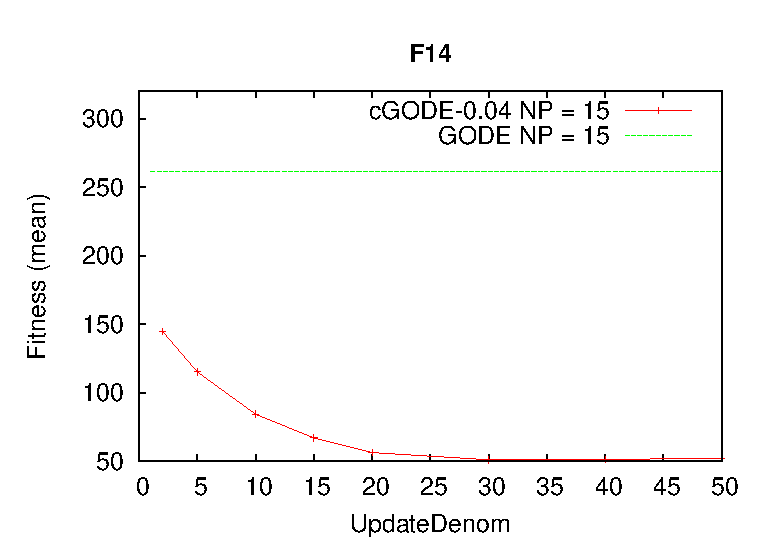
\includegraphics[width=0.37\textwidth]{images/Update/GODE/Update_GODE_F14_15.eps} & 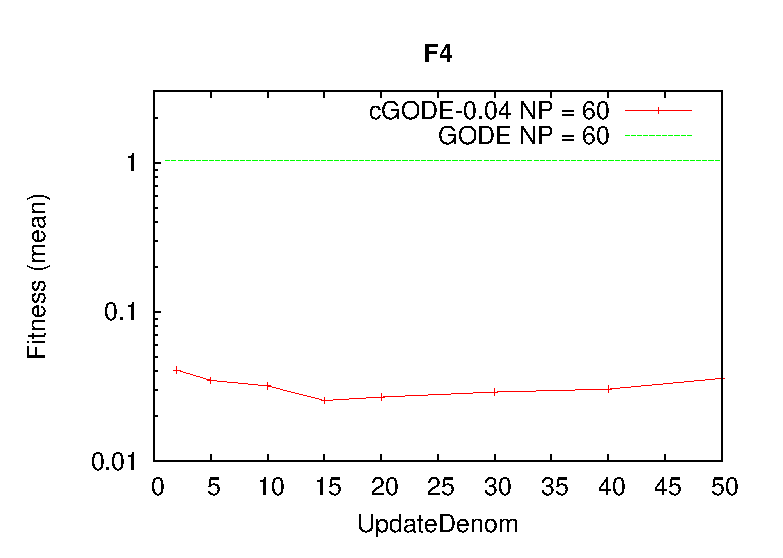
\includegraphics[width=0.37\textwidth]{images/Update/GODE/Update_GODE_F4_60.eps}  \\
  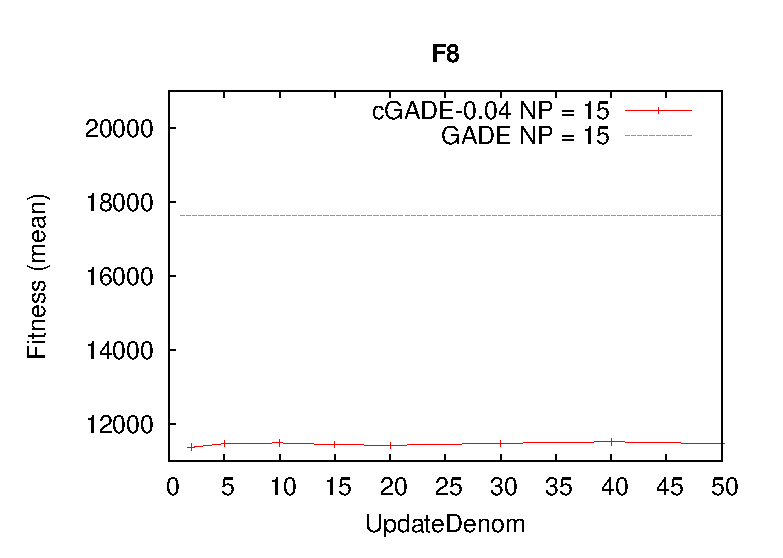
\includegraphics[width=0.37\textwidth]{images/Update/GADE/Update_GADE_F8_15.eps} & 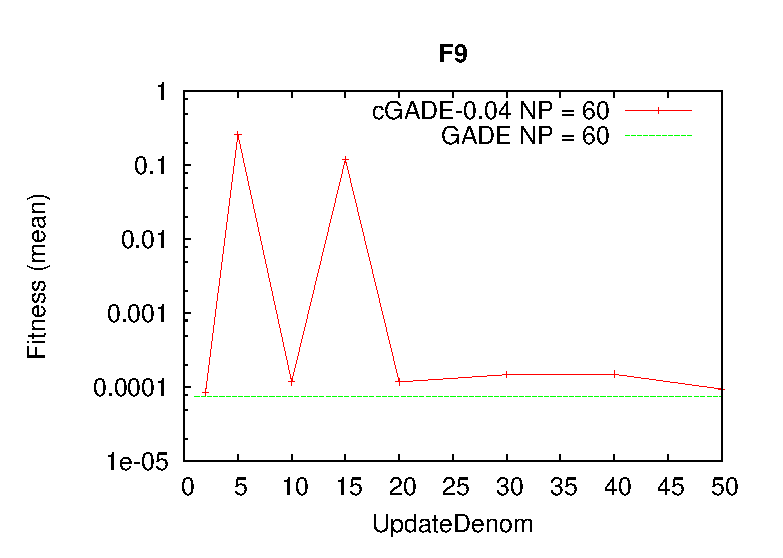
\includegraphics[width=0.37\textwidth]{images/Update/GADE/Update_GADE_F9_60.eps}  \\
\end{tabular}
\caption{Mean of the fitness obtained with different $UpdateDenom$ values}
\label{fig:updateDenom}
\end{figure}

\textcolor{red}{
Figure~\ref{fig:updateDenom} shows the mean obtained with the different $UpdateDenom$ values in four illustrative cases that appeared repeatedly.
%
In each case, the mean obtained by the model that does not incorporate our proposals is also shown.
%
In the case of applying c\textsc{gode-0.04} with $NP = 15$ to the problem \textsc{f14}, we can appreciate that the largest $UpdateDenom$ value provokes
the lowest mean value.
%
This happens because c\textsc{gode} with a low population size induce a too large degree of intensification, so inducing a slow update mechanism provokes a useful exploration.
%
In other cases, as expected, the intermediate values of $UpdateDenom$ are the ones that result in a better quality.
%
This happens for instance when c\textsc{gode} with $NP = 60$ is applied to \textsc{f4}.
%
We also identified some cases where the quality does not depend practically on the $UpdateDenom$ value.
%
For instance, this arose when applying c\textsc{gade} with $NP = 15$ to \textsc{f8}.
%
In such a case, the only statistically significant difference appear when comparing the scheme with $UpdateDenom = 2$ with the one that uses $UpdateDenom = 50$.
%
In cases like this one, most of the benefits come from the continuation scheme and not from the large mutations, so even if the scheme is executed by setting \HMR{} to 0,
high-quality values are obtained.
%
In all the previous cases, our proposals provided benefits regardless of the $UpdateDenom$ value applied.
%
However, as we have shown, in a minority of cases our proposals provoke some degradation.
%
For instance, this is the case of c\textsc{gade} with $NP = 60$ for \textsc{f9}.
%
In such cases, by modifying the $UpdateDenom$ value, some improvements can be obtained.
%
However, we could not obtain significant improvements when compared to the basic schemes that do not incorporate our proposals.
%
This means that when dealing with new problems, the practitioners can test the schemes practically with any $UpdateDenom$ value to check if our proposals
provides benefits or not.
%
If the scheme provide significant benefits, it might make sense to tune the $UpdateDenom$ value.
%
Otherwise, the scheme might be already explorative enough, so testing different $UpdateDenom$ values is not so promising.
}

\subsection{Seventh Set of Experiments: Other Benchmarks}

\begin{table}[!t]
%\renewcommand{\arraystretch}{1.4}
\caption{Comparison of errors obtained by \textsc{DE} and \textsc{CDE}-0.04 in 3,000,000 evaluations with the CEC'10 Benchmark Test Suite}
\label{tab:scalability_1000_cec}
\centering
\begin{scriptsize}
\begin{tabular}{c || c c c | c c c c}
\hline
 & \multicolumn{3}{|c|}{\textsc{de}} & \multicolumn{4}{|c}{\textsc{cde}} \\ \hline
    & Median                 & Mean                  & Std. Dev.             & Median                         & Mean                           & Std. Dev.                      & Stat.               \\ \hline
F1  & $4.17 \cdot 10^{-17}$ & $2.56  \cdot 10^{5}$  & $5.39 \cdot 10^{6}$  & $\mathbf{6.84 \cdot 10^{-21}}$ & $\mathbf{1.33 \cdot 10^{1}}$  & $\mathbf{2.55 \cdot 10^{2}}$ & $\uparrow$ \\ \hline
F2  & $1.11 \cdot 10^{2}$   & $1.11  \cdot 10^{2}$  & $2.90 \cdot 10^{1}$  & $\mathbf{3.48 \cdot 10^{1}}$   & $\mathbf{3.53 \cdot 10^{1}}$  & $\mathbf{8.40}$ & $\uparrow$ \\ \hline
F3  & $1.74 \cdot 10^{-13}$ & $3.67  \cdot 10^{-2}$ & $2.10 \cdot 10^{-1}$ & $\mathbf{1.03 \cdot 10^{-13}}$ & $\mathbf{1.17 \cdot 10^{-4}}$ & $\mathbf{7.7 \cdot 10^{-4}}$ & $\uparrow$ \\ \hline
F4  & $4.29 \cdot 10^{13}$  & $4.30  \cdot 10^{13}$ & $8.44 \cdot 10^{12}$ & $4.21 \cdot 10^{13}$  & $4.25 \cdot 10^{13}$ & $8.63 \cdot 10^{12}$ & $\leftrightarrow$ \\ \hline
F5  & $1.70 \cdot 10^{8}$   & $1.70  \cdot 10^{8}$  & $2.43 \cdot 10^{7}$  & $1.69 \cdot 10^{8}$   & $1.69 \cdot 10^{8}$  & $2.45 \cdot 10^{7}$ & $\leftrightarrow$ \\ \hline
F6  & $1.35 \cdot 10^{3}$   & $9.84  \cdot 10^{4}$  & $3.46 \cdot 10^{5}$  & $\mathbf{9.52 \cdot 10^{2}}$   & $\mathbf{8.58 \cdot 10^{4}}$  & $\mathbf{3.38 \cdot 10^{5}}$ & $\uparrow$ \\ \hline
F7  & $1.46 \cdot 10^{7}$   & $1.80  \cdot 10^{7}$  & $3.14 \cdot 10^{7}$  & $\mathbf{1.42 \cdot 10^{7}}$   & $\mathbf{1.71 \cdot 10^{7}}$  & $\mathbf{1.22 \cdot 10^{7}}$ & $\uparrow$ \\ \hline
F8  & $4.85 \cdot 10^{7}$   & $1.33  \cdot 10^{11}$ & $1.92 \cdot 10^{12}$ & $\mathbf{4.68 \cdot 10^{7}}$   & $\mathbf{6.69 \cdot 10^{7}}$  & $\mathbf{3.63 \cdot 10^{7}}$ & $\uparrow$ \\ \hline
F9  & $8.41 \cdot 10^{8}$   & $8.39  \cdot 10^{8}$  & $5.61 \cdot 10^{7}$  & $\mathbf{8.35 \cdot 10^{8}}$   & $\mathbf{8.35 \cdot 10^{8}}$  & $\mathbf{5.67 \cdot 10^{7}}$ & $\uparrow$ \\ \hline
F10 & $5.02 \cdot 10^{3}$   & $5.01  \cdot 10^{3}$  & $2.15 \cdot 10^{2}$  & $\mathbf{4.99 \cdot 10^{3}}$   & $\mathbf{5.00 \cdot 10^{3}}$  & $\mathbf{2.13 \cdot 10^{2}}$ & $\uparrow$ \\ \hline
F11 & $2.062 \cdot 10^{2}$  & $2.05  \cdot 10^{2}$  & $3.29$               & $\mathbf{2.061 \cdot 10^{2}}$  & $\mathbf{2.04 \cdot 10^{2}}$  & $\mathbf{3.65}$ & $\uparrow$ \\ \hline
F12 & $7.62 \cdot 10^{5}$   & $7.60  \cdot 10^{5}$  & $3.28 \cdot 10^{4}$  & $\mathbf{7.55 \cdot 10^{5}}$   & $\mathbf{7.54 \cdot 10^{5}}$  & $\mathbf{3.09 \cdot 10^{4}}$ & $\uparrow$ \\ \hline
F13 & $1.64 \cdot 10^{3}$   & $1.45  \cdot 10^{7}$  & $1.76 \cdot 10^{8}$  & $\mathbf{1.15 \cdot 10^{3}}$   & $\mathbf{1.62 \cdot 10^{3}}$  & $\mathbf{1.59 \cdot 10^{3}}$ & $\uparrow$ \\ \hline
F14 & $1.28 \cdot 10^{9}$   & $1.28  \cdot 10^{9}$  & $5.88 \cdot 10^{7}$  & $\mathbf{1.27 \cdot 10^{9}}$   & $\mathbf{1.26 \cdot 10^{9}}$  & $\mathbf{5.90 \cdot 10^{7}}$ & $\uparrow$ \\ \hline
F15 & $1.20 \cdot 10^{4}$   & $1.20  \cdot 10^{4}$  & $3.82 \cdot 10^{2}$  & $1.20 \cdot 10^{4}$   & $1.20 \cdot 10^{4}$  & $3.73 \cdot 10^{2}$ & $\leftrightarrow$ \\ \hline
F16 & $4.142 \cdot 10^{2}$  & $4.127 \cdot 10^{2}$  & $3.58$               & $\mathbf{4.141 \cdot 10^{2}}$  & $\mathbf{4.124 \cdot 10^{2}}$ & $\mathbf{3.85}$ & $\uparrow$ \\ \hline
F17 & $1.72 \cdot 10^{6}$   & $1.72  \cdot 10^{6}$  & $5.23 \cdot 10^{4}$  & $\mathbf{1.70 \cdot 10^{6}}$   & $\mathbf{1.69 \cdot 10^{6}}$  & $\mathbf{5.06 \cdot 10^{4}}$ & $\uparrow$ \\ \hline
F18 & $6.55 \cdot 10^{3}$   & $3.09  \cdot 10^{7}$  & $1.53 \cdot 10^{8}$  & $\mathbf{3.25 \cdot 10^{3}}$   & $\mathbf{4.53 \cdot 10^{3}}$  & $\mathbf{3.26 \cdot 10^{3}}$ & $\uparrow$ \\ \hline
F19 & $4.64 \cdot 10^{6}$   & $4.63  \cdot 10^{6}$  & $2.63 \cdot 10^{5}$  & $\mathbf{4.62 \cdot 10^{6}}$   & $\mathbf{4.61 \cdot 10^{6}}$  & $\mathbf{2.73 \cdot 10^{5}}$ & $\uparrow$ \\ \hline
F20 & $2.07 \cdot 10^{3}$   & $4.10  \cdot 10^{7}$  & $2.54 \cdot 10^{8}$  & $\mathbf{1.71 \cdot 10^{3}}$   & $\mathbf{1.73 \cdot 10^{3}}$  & $\mathbf{3.76 \cdot 10^{2}}$ & $\uparrow$ \\ \hline
\end{tabular}
\end{scriptsize}
\end{table}





This last experiment is devoted to demonstrating the generality of the weaknesses of \DE{} that have been analyzed in this
paper, and the suitability of our schemes for dealing with other problems of varying complexity.
%
As was explained earlier, the \textsc{cec'10} tests were selected for this purpose
because the features that characterize them are different from those of the \textsc{soco} tests.
%
For instance, it is known that in the \textsc{soco} tests, ``mutating a contiguous sequence of components is somehow more effective''~\cite{Zhao:13}, meaning
that the exponential crossover is highly suitable. % for the test problems adopted here.
%
However, in the \textsc{cec'10} benchmark, using a combination of bin and exp crossover seems more effective~\cite{Brest:10,Wang:10}.
%
In our scheme, the exp and bin operators considered $CR$ values equal to 0.5 and 0.1, respectively.
%
Several other modifications specifically designed for this benchmark have been devised~\cite{Brest:10,Brest:12}.
%
\textcolor{red}{
For instance, in~\cite{Brest:12} the parameter control strategies were modified by using certain threshold values at specific stages
of the optimization process.
%
In addition, ageing, adaptation of the scale factor sign, self-adaptation, local search and several mutation strategies were taken into account.
%
In this experiment, our purpose is just to show that \DE{} is also affected by the weaknesses analyzed herein when dealing with the \textsc{cec'10} benchmark,
so we decided to operate with a simple baseline scheme, meaning that these additional modifications were not included.
%
Thus, the only modification with respect to the basic \DE{} used in our initial experiments is the integration of the bin crossover.
}

Table~\ref{tab:scalability_1000_cec} shows the mean, median and standard deviation
of \DE{} and \CDE{}-0.04 in 3$\,$000$\,$000 function evaluations.
%
This stopping criterion was the one proposed during the competition held in \textsc{cec'10}, so it was selected with the aim of facilitating
the comparisons between different models.
%
The format of the table is similar to that used in previous sections.
%
We can see that the new model provides significant benefits in most problems.
%
In fact, statistical tests report that \CDE{}-0.04 is significantly better than \DE{} in 17 out of 20 problems.
%
As in previous experiments, there are several cases where \DE{} has a much larger mean value than the one attained by \CDE{}-0.04
--- for instance F1, F8, F13 and F18 --- meaning
that the drawbacks analyzed also appear in this benchmark, and that they can be alleviated using the schemes proposed in this paper.

%Finally, we would like to note that the results we obtained were quite promising when compared with simple mechanisms 
%, even though our scheme was not provided with other promising components, such as
%parameter control or intensification schemes.
%
%For instance, our medians are better than those reported in~\cite{Wang:10} for 9 problems.
\textcolor{red}{
Finally, we would like to note that while our proposals provided significant benefits in the baseline \DE{},
the results are not as good as those reported in complex hybrid schemes~\cite{Brest:12,LaTorre:12}. 
%
In fact, in none of the problems our simple scheme obtained lower mean or median values than the ones reported in~\cite{Brest:12}.
%
This was expected because we have not made an effort to adapt our scheme to the specific nature of this benchmark,
while in~\cite{Brest:12} several adaptations specifically designed for these problems were included.
%
%Since the method in~\cite{Brest:12} is not freely available, we could not easily integrate our proposals with it.
%
We did some additional experiments with the schemes used for the \textsc{soco} tests.
%
Similarly to what happened in our previous experiments, results could be improved and our proposals provided clear benefits.
%
Thus, similar conclusions than for the \textsc{soco} tests can be drawn.
%
However, the results obtained were far from the ones attained in~\cite{Brest:12}.
%
The reason is that most of the methods used for the \textsc{soco} tests must be adapted to perform properly when the \textsc{cec}
tests are considered~\cite{LaTorre:14}.
}
%

\section{Conclusions and Future Work}
\label{sec:conc}

\DE{} is a highly efficient and popular metaheuristic especially tailored for continuous optimization problems.
%
The analyses developed with \DE{} in recent decades have shown that this metaheuristic suffers from
the curse of dimensionality, i.e., its performance deteriorates rapidly when dealing with large-scale problems.
%
In this paper, the relationship between certain weaknesses that had been detected by several authors and the use
of large dimensionalities is explored.
%
The weaknesses are related to the limited number of trial vectors that can be generated in \DE{}, and to the
less expansive behavior that \DE{} shows with respect to other metaheuristics.

\textcolor{red}{
The main effects of these weaknesses can be avoided when using low-dimensional problems by 
increasing the diversity induced by \DE{}, which is usually done by increasing the
population size.
}
%
However, when dealing with large-scale problems, increasing the population size is not a proper choice
as faster convergence is required, given the fact that the portion of space being explored is much lower.
%
In addition, the mathematical analysis presented in this paper provides better insight into the reasons
for the appearance of these drawbacks when dealing with high-dimensional spaces.
%
The mathematical analysis also shows that by using a variable mutation
scale factor, these problems can be partially alleviated.
%
However, these schemes introduce large changes into the basic behavior of \DE{},
the benefits of which are not so clear.

Several different ways of avoiding these weaknesses might be proposed.
%
In this paper, two schemes that can be used simultaneously have been devised.
%
While these schemes represent by themselves, an important advance in the field,
the main contribution of this paper is that with the help of the new methods, we have
shown that the drawbacks analyzed herein have a significant effect on the behavior of \DE{}, especially when
high-dimensional spaces are involved.
%
For this reason, the findings detailed in this paper should be taken into account in the future when designing new \DE{} schemes.
%
The first devised method has the effect of increasing the number of potential vectors that can be
generated in \DE{} while at the same time, respecting the basic principles of \DE{}.
%
The second modification increases the explorative behavior of \DE{} by promoting large perturbations
with an adaptive scheme.
%
%The schemes are applied when trial vectors take only one variable from the mutant vectors.
%
%Thus, the probability of applying them depends on the crossover rate considered.

Computational results from a large set of scalable problems with various
complexities show that the new proposal is much better
than the original \DE{} scheme.
%
The benefits obtained in terms of the quality of the solutions are clear.
%
Moreover, the number of resources that can be saved with the new scheme is significant.
%
Comparisons with several \DE{} variants that consider a variable scale factor showed
the higher effectiveness of the new scheme.
%
Along the same line as other researches, this latest study also calls
into question the robustness of the adaptive schemes
that use feedback to set the value of the mutation scale factor.
%
\textcolor{red}{
Experiment with several complex non-hybrid \DE{} variants have also been included.
%
In such cases, the benefits remain intact, so the state-of-the-art non-hybrid \DE{} schemes
for the \textsc{soco} tests could be improved. 
%
In the basic \DE{} variant the benefits of the proposals vanish when dealing with larger population sizes.
%
However, when more complex \DE{} variants were applied, the benefits of our proposals also appeared when 
dealing with large populations.
%
The reason is that such state-of-the-art schemes induce a larger degree of exploitation.
%
Thus, the advantages reported depend on such a degree, being more useful when exploitative schemes
are taken into account.
}
%
%The study also shows that benefits can be obtained for large ranges of crossover rates.
%
%Thus, even when the schemes are only occasionally applied, the effects on the results are significant.
%
Finally, the scalability study demonstrates that as the dimensionality of the problems involved increases, the
advantages of the proposals are more significant.
%
In these cases, the worst-case behavior of \DE{} can be significantly improved by considering the
schemes proposed herein.

Several lines of future work might be explored.
%
First, similar modifications to those we propose might be applied when the trial
vectors take several variables from the mutant vectors.
%
\textcolor{red}{
Since the distributions associated to the different variables are not independent, 
their dependencies should be modeled.
%
One choice might be to use copula functions.
}
%
%This might be done in several ways and is closely related to the dither and jitter schemes,
%so some studies in this area might be in order.
%In order to do this, the 
%
Another line of future work is to combine the proposals described here with some other methods
that have been proposed in the literature.
\textcolor{red}{
%
First, since in our opinion the global search capabilities of \DE{} can already be improved, we would like to combine
our methods with some general diversity-preservation strategies.
%
Specifically, since our schemes operate on the variation stage, incorporating some of the ones that operate
on the replacement phase seems truly promising.
%
Once this has been done, merging the scheme with co-evolution and with local search schemes
seems very promising.
%
The incorporation of such techniques might result in more robust and competitive schemes.
}
%
Finally, since some questions concerning the robustness of using feedback to set the mutation scale factor
have emerged both in this work and in other related research, conducting more detailed analyses on this topic might
be highly beneficial to the \DE{} community.

% if have a single appendix:
%\appendix[Proof of the Zonklar Equations]
% or
%\appendix  % for no appendix heading
% do not use \section anymore after \appendix, only \section*
% is possibly needed

% use appendices with more than one appendix
% then use \section to start each appendix
% you must declare a \section before using any
% \subsection or using \label (\appendices by itself
% starts a section numbered zero.)
%


%\appendices
%\section{Proof of the First Zonklar Equation}
%Appendix one text goes here.

% you can choose not to have a title for an appendix
% if you want by leaving the argument blank
%\section{}
%Appendix two text goes here.


% use section* for acknowledgement
\section*{Acknowledgment}
The first author acknowledges the financial support from CONCYTEG as part of the plan ``Investigadores J\'ovenes - DPP-2014''.
The second author is also affiliated to the
UMI LAFMIA 3175 CNRS at CINVESTAV-IPN.
He also acknowledges the financial support from CONACyT project no. 221551.


\bibliography{InfSci-14-segura}

\end{document}
